\hypertarget{sec:awsm-rm}{%
\chapter{AWSM Risk Management Method}\label{sec:awsm-rm}}

This chapter addresses research objective \cref{ro:2}:

\begin{quote}
To enable demonstration of desirability and feasibility of a potential \glslink{web}{Web}-based version of the \gls{Legacy System} with limited resources and lack of \gls{Web Engineering} expertise.
\end{quote}

First, the current situation is briefly analyzed to identify requirements and review related work.
Three research questions are derived from \cref{ro:2}, inspired by the analysis results. 
To address the research questions, three sections outline the three main contributions towards \cref{ro:2} in the context of the AWSM:RM method: the novel concept of \gls{Rapid Web Migration Prototyping} is introduced and a process for rapid, semi-automatic creation of \gls{Web Migration} prototypes is described, a technique for business logic reuse in \glspl{web migration prototype} based on \glslink{wasm}{WebAssembly} is presented, and a technique for automatic \gls{Transformation} of legacy user interface to \glslink{web}{Web}-based user interface prototypes is described.
Finally, the method is evaluated against the requirements, and the evaluation is supported by three experiments, which include analysis of both empirical evaluations and objective measurements.

\hypertarget{sec:rm.analysis}{%
\section{Analysis}\label{sec:rm.analysis}}
\vspace{15pt}

The following analysis briefly summarizes the situation of doubts about desirability and feasibility of a \webbased version of the \gls{Legacy System} and the challenges of demonstrating these properties through application of \gls{Rapid Prototyping} in the \gls{Web Migration} domain.
Requirements are derived from this analysis and an overview of related work on the two key paradigms used for AWSM:RM is given.

\vspace{-15pt}
\subsection{Situation and Challenges}
\vspace{10pt}

Our field research  has revealed \emph{doubts about desirability} and \emph{doubts about feasibility} as two major factors rendering \glspl{isv} hesitant to commence a \gls{Web Migration}, as described in \cref{sec:problem-analysis-results}.
\emph{Feasibility studies} are the most common \gls{risk management} approach, employed by 7 of the 23 approaches assessed in \cref{sec:approaches}.
They are often conducted as \emph{pilot migration projects}, i.e.~migration trials with a restricted scope that migrate a small portion of the \gls{Legacy System} in order to identify insuperable technical obstacles as early as possible \autocite{Sneed2010SoftwareMigration}, to test the migration process and toolchain \autocite{AmazonWebServices2018Migration} and to facilitate an informed decision in favour or against commencing a full-scale migration \autocite{Sneed2010SoftwareMigration}.
%Examples of this can be seen in the ``first migrations'' of AWS Migration \autocite{AmazonWebServices2018Migration}, SMART-MP \autocite{CMUSoftwareEngineeringInstitute2013a} in SMART \autocite{Lewis2005SMART,Lewis2008SMART} and the experimentation-based feasibility studies in IC4 \autocite{Fowley2018Experimentation}.
However, these feasibility studies and migration pilots put the main focus on the technical feasibility of the migration itself.
They fail to create \emph{concrete and tangible results} that allow assessing the \emph{plausibility of a \glslink{web}{Web}-based version} of the \gls{Legacy System} and the desirability with regard to \emph{advantages of \glspl{Web System}}, leading to a gap as identified in \cref{g:2}.
\vspace{-5pt}

In \gls{Forward Engineering}, Prototyping \autocite{Wallmueller2001SoftwareQuality} and in particular \emph{\gls{Rapid Prototyping}} \autocite{ISO/IEEE24765Vocabulary,Gordon1995RapidPrototyping} is used as \emph{effective \gls{risk management} technique} \autocite{Wallmueller2001SoftwareQuality} for risk reduction \autocite{ISO/IEEE24765Vocabulary} to address desirability and feasibility in early stages, allowing to create a running software prototype as concrete and tangible result \autocite{Alavi1984}.
\gls{Prototyping} is particularly appropriate for unfamiliar situations with limited experience to draw from \autocite{Tripp1990}, like the new target environment in \gls{Web Migration}, which significantly differs from the \glslink{Legacy System}{legacy} \gls{Desktop Application} environment.
In \gls{Web Engineering}, quick creation of cheap, throw-away versions representing the core functionality and characteristics of the envisioned \gls{Web System} has become industry practice as it enables discussing solution alternatives and facilitates communication with stakeholders \autocite{Alavi1984,HCD2015}.
This communication and risk reduction can accelerate \glslink{Software Modernization}{modernization} plans \autocite{ForresterResearch2011Modernization} by addressing resistance within the organization \autocite{Khadka2014ProfessionalsModernization,Sneed2010ReMiP} making reasons and consequences of \glslink{Software Modernization}{modernization} visible.
In this way, prototypes represent a concrete and tangible contribution to the \gls{business case} that serves as a means of communication for stakeholders to support decision making.
Transfer of these potential benefits into the \gls{Web Migration} domain is the primary motivation of AWSM:RM.
\vspace{-5pt}

\gls{Web Migration}, however, is inherently different from forward \gls{Web Engineering}.
While a prototype in forward \gls{Web Engineering} is created from scratch based on early and potentially unclear versions of requirements, a \emph{\gls{web migration prototype}} is built based on elaborate requirements represented by and potentially recovered from an existing and mature \gls{Legacy System} already known to stakeholders and source of their expectations.
This \emph{brownfield} \autocite{Hopkins2008Brownfield} situation constitutes the main difference between \gls{Web Migration} and forward \gls{Web Engineering}.
An \gls{isv} employing \gls{Rapid Prototyping} for forward \gls{Web Engineering} can rely on a staff base with \gls{Web Engineering} expertise that can leverage open \gls{web} standards like \gls{http}, \gls{html}, \gls{css}, JavaScript and popular \gls{web} Development platforms and frameworks like node.js\footnote{\url{https://nodejs.org/} Retrieved: 6.12.2019}, Rails\footnote{\url{https://rubyonrails.org/} Retrieved: 6.12.2019}, React\footnote{\url{https://reactjs.org/} Retrieved: 6.12.2019}, Angular\footnote{\url{https://angular.io/} Retrieved: 6.12.2019} to quickly create running prototypes.
In contrast, an \gls{isv}, as described in \cref{sec:company-characteristics}, has a staff base with expertise in \glslink{Legacy System}{legacy} platforms like C, \cpp, Java and \gls{Desktop Application} frameworks like \gls{mfc}, WPF\footnote{\url{https://msdn.microsoft.com/en-us/library/aa663364.aspx} Retrieved: 6.12.2019}, Swing\footnote{\url{https://docs.oracle.com/javase/8/docs/technotes/guides/swing} Retrieved: 6.12.2019}.

\gls{Rapid Prototyping} is, therefore, not directly applicable to \gls{Web Migration}.
The \gls{Rapid Prototyping} paradigm needs to be adapted to the characteristics of migration and the situation of \glspl{isv} with non-\glslink{web}{Web} \glslink{Legacy System}{legacy} \glslink{Desktop Application}{desktop software}, following principle \cref{p:4}.
Thus, the challenge addressed by AWSM:RM in order to achieve \cref{ro:2} is to specify a suitable \gls{risk management} method for quick creation of concrete, tangible prototypes of a \glslink{web}{Web}-based version of the legacy \glslink{Desktop Application}{desktop system} that can be used to demonstrate desirability and feasibility for communication decision making of migration stakeholders with limited resources and \gls{Web Engineering} expertise.

\vspace{-15pt}
\hypertarget{sec:rm.requirements}{%
\subsection{Requirements}\label{sec:rm.requirements}}
\vspace{5pt}

The following requirements specify \cref{ro:2}, based on the analysis presented above and the \gls{awsm} principles.

\textbf{Effectiveness}. Risk management should be enabled through the creation of concrete, tangible results allowing to demonstrate desirability and feasibility of \gls{Web Migration}.

\vspace{-10pt}
\textbf{Efficiency}. Creation of \glspl{web migration prototype} should be supported by tools to require fewer resources compared to manual creation.

\vspace{-10pt}
\textbf{Expertise}. Creation of \glspl{web migration prototype} should be feasible with available expertise of the \gls{isv}'s staff.

\vspace{-10pt}
\textbf{Reuse}. Creation of \glspl{web migration prototype} should reuse existing functionality from the source \gls{Legacy System}.

\vspace{-10pt}
\textbf{Plausibility}. The \glspl{web migration prototype} should enable assessment of the plausibility of a \glslink{web}{Web}-based version of the \gls{Legacy System} by representing significant architectural changes: Client/Server communication, URL-based navigation, and \gls{ui} Rendering in a \gls{web} browser.

\vspace{-15pt}
\hypertarget{sec:awsm-rm:related-work}{%
\subsection{Related Work}\label{sec:awsm-rm:related-work}}
\vspace{10pt}

This section introduces \gls{Prototyping} and \gls{Rapid Prototyping} as key paradigms of AWSM:RM.
It establishes the semantics of the key terminology of \gls{Prototyping} used in the following description of AWSM:RM and provides a minimal overview of related work in these fields.
%\textbf{Prototyping in Software Engineering} is an established practice for requirements clarification and validation of understanding of elicited requirements \autocite{SWEBOK2014,Wood1992Prototyping}.
%Prototypes can range from paper \emph{mockups} \autocite{ISO/IEEE24765Vocabulary} to beta-test versions of software products and exist in different styles, varying from throw-away to evolutionary, depending on the particular prototyping life cycle process \autocite{SWEBOK2014}.

\textbf{Prototyping} is a risk reduction method  \autocite{ISO/IEEE24765Vocabulary}
defined as:
\vspace{-10pt}

\begin{thesisdefinition}{Software Prototyping \autocite{SWEBOK2014}}{def:prototyping}
Software prototyping is an activity that generally creates incomplete or minimally functional versions of a software application, usually for trying out specific new features, soliciting feedback on software requirements or user interfaces, further exploring software requirements, software design, or implementation options, and/or gaining some other useful insight into the software.
\end{thesisdefinition}

%From the software maintenance perspective, \gls{Prototyping} is an activity of feasibility analysis \autocite{IEEE1219Maintenance}.
Software prototypes represent a \emph{functional, demonstrative product}, proving ``the relevance of a solution'' \autocite{ISO/IEEE24765Vocabulary}.
%Prototyping is a method for improving software quality \autocite{Wallmueller2001SoftwareQuality} and has been acknowledged to increase the efficiency and effectiveness of software design \autocite{Tripp1990}.
\emph{Explorative \gls{Prototyping}} seeks to integrate user feedback in the design process and creates \emph{horizontal prototypes}, which focus on user interaction \autocite{Wallmueller2001SoftwareQuality}.
A \emph{demonstrative prototype} communicates ideas of the user interface and capabilities of the envisioned system, allowing decision makers to assess desirability and benefits \autocite{Wallmueller2001SoftwareQuality}.
%With its intrinsic communication value, \gls{Rapid Prototyping} has been used in \gls{hci}-related fields such as \gls{ui} and Instructional Design.
%\gls{Rapid Prototyping} of \emph{\gls{ui} Designs} was proposed by the \emph{CrowdDesign} approach \autocite{Nebeling2012} already discussed in \cref{sec:re.related}.
%Tripp et al.~transfer \gls{Rapid Prototyping} to \emph{Instructional Design}, i.e.~the design of instructional systems \autocite{Tripp1990}, to foster the participation of users in the design process.

\textbf{\gls{Rapid Prototyping}} is widely used in Agile Software Development, as it suits the ``working software over comprehensive documentation'' value \autocite{Fowler2001} and the principles of continuous and frequent delivery of valuable software, collaboration of business people and developers and working software as primary measure of progress of the Agile Manifesto\footnote{\url{https://agilemanifesto.org/} Retrieved: 6.12.2019}.
\gls{Rapid Prototyping} can be used as a starting point for Agile \gls{mdwe} as in MockupDD \autocite{Rivero2013MockupDD,Rivero2013,Rivero2014Electra}.
\gls{Rapid Prototyping} is defined as follows:

\vspace{-10pt}
\begin{thesisdefinition}{Rapid Prototyping \autocite{ISO/IEEE24765Vocabulary}}{def:rapidprototyping}
type of prototyping in which emphasis is placed on developing prototypes early in the development process to permit early feedback and analysis in support of the development process
\end{thesisdefinition}

\emph{\gls{Prototyping} in Web Migration}, in contrast, has not received much attention.
Among the \gls{Web Migration} approaches assessed in \cref{sec:approaches}, only IC4 \autocite{Fowley2017CloudSME} proposes the use of prototypes in cloud migration.
%While the target beneficiary of IC4 is similar to the \gls{sme}-sized \gls{isv} described in \cref{sec:company-characteristics}, IC4's use of \gls{Prototyping} belongs to the experimental \gls{Prototyping} \autocite{Wallmueller2001SoftwareQuality} category.
IC4 prototypes, however, focus on technical feasibility; prototypes are created to compare different \gls{Reengineering} options and create performance benchmarks.
IC4 takes a more coarse-grain perspective comparing top-level architectural decisions regarding component allocation, e.g.~virtualized relational database vs.~\gls{paas} SQL services vs.~NoSQL.
To a lesser extent, rapid relocation approaches like AppCloak \autocite{Tak2014} can be considered a form of \gls{Rapid Prototyping} for \gls{Web Migration} as they allow to quickly create \gls{web} (cloud-based for AppCloak) versions of \glslink{Legacy System}{legacy} \glspl{Desktop Application}.
However, the focus is on technical benchmarks, and the disadvantages of \gls{Encapsulation} approaches, as discussed in \cref{sec:sota.discussion}, apply.
Other \gls{Web Migration} methodologies fail to address benefits and early customer feedback in pre-migration phases.
\vspace{-4pt}
%Comprehensive \gls{Web Migration} methodologies like ARTIST focus on technical feasibility and fail to address benefits and early customer feedback in pre-migration phases \autocite{ARTIST2014Methodology}.

Due to the success of \gls{Rapid Prototyping} in achieving similar goals -- demonstration of an envisioned software for communication, feedback and decision making -- in \gls{Forward Engineering}, \cref{sec:rwmp} describes the application of \gls{Rapid Prototyping} in \gls{Web Migration} by specification of a technique for creating demonstrative, functional, horizontal prototypes based on existing \glspl{Legacy System}.
%The following section introduces the \gls{Rapid Prototyping}-based Risk Management of AWSM:RM.

\vspace{-28pt}
\hypertarget{sec:rm.research-questions}{%
\section{Research Questions}\label{sec:rm.research-questions}}
\vspace{10pt}

The analysis presented above raises three research questions:

\begin{quote}
\textbf{AWSM:RM Research Question RQ1}: How to demonstrate desirability and feasibility of a potential \glslink{web}{Web}-based version of the \gls{Legacy System} with limited resources and lack of \gls{Web Engineering} expertise?
\end{quote}
\vspace{-4pt}

\begin{quote}
\textbf{AWSM:RM Research Question RQ2}: How to transfer the \gls{Rapid Prototyping} paradigm into a \gls{Web Migration} context?
\end{quote}
\vspace{-4pt}

\begin{quote}
\textbf{AWSM:RM Research Question RQ3}: How to provide guidance and automation for \gls{Rapid Web Migration Prototyping} to enable execution with limited \gls{Web Engineering} and \gls{Web Migration} expertise?
\end{quote}
\vspace{-4pt}

To design and evolve a solution for research objective \cref{ro:2}, this chapter addresses these three research questions in the following sections.

\vspace{-15pt}
\hypertarget{sec:rwmp}{%
\section{Rapid Web Migration Prototyping}\label{sec:rwmp}}
\vspace{15pt}

To enable the demonstration of desirability and feasibility of a potential \glslink{web}{Web}-based version of the \gls{Legacy System} set as research objective \cref{ro:2}, AWSM:RM allows rapid creation of a \glslink{web}{Web}-based functional demonstrative prototype of the \gls{Legacy System} in early stages of \gls{Web Migration}.
It provides an answer to AWSM:RM RQ1.
Addressing the resources and expertise constraint of \cref{ro:2}, AWSM:RM defines reuse-based techniques and tools which allow the creation of such prototypes with limited resources and lack of \gls{Web Engineering} expertise. \Cref{sec:rwmp.overview} provides an overview of the method, \cref{sec:rwmp.integration} addresses integration of the method with ongoing development activities, and \cref{sec:mockapi} describes the use and adaption of an existing method for \gls{api} prototyping.

\vspace{-10pt}
\hypertarget{sec:rwmp.overview}{%
\subsection{Overview}\label{sec:rwmp.overview}}
\vspace{10pt}

This section presents an overview of the AWSM:RM method and its related tools as visualized in \cref{fig:awsm.rm.overview}.

\begin{figure}[h!]
\hypertarget{fig:awsm.rm.overview}{%
\centering
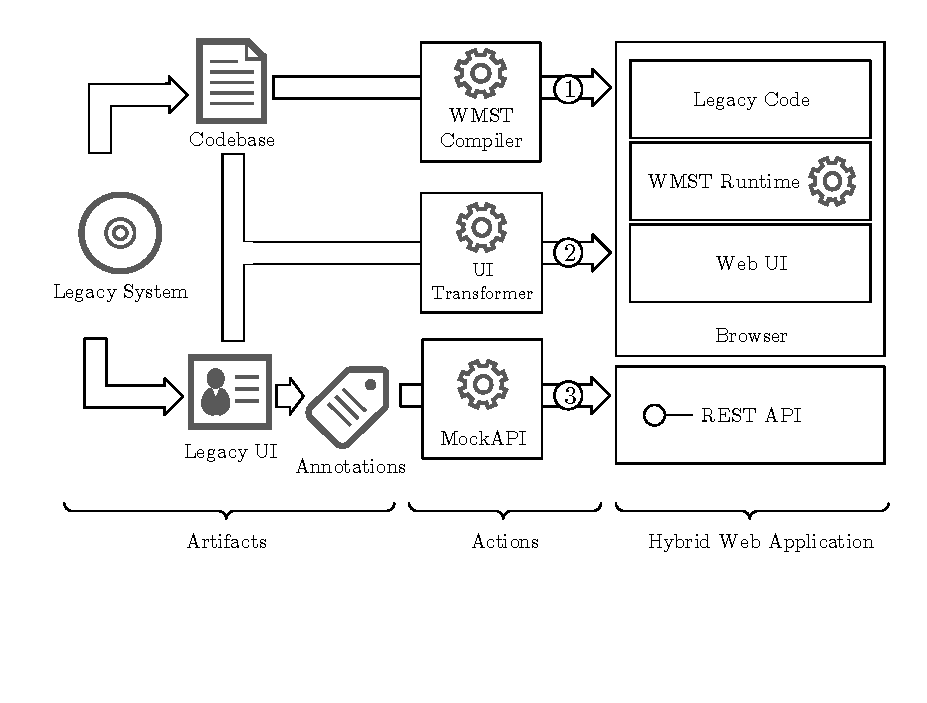
\includegraphics[width=0.95\textwidth]{../figures/rewamp/wms3.pdf}
\caption{AWSM:RM Prototyping Overview}\label{fig:awsm.rm.overview}
}
\end{figure}

The core idea of AWSM:RM is to transfer \gls{Rapid Prototyping} to the \gls{Web Migration} domain, answering AWSM:RM RQ2.
AWSM:RM is a method realizing the novel concept of \emph{\gls{Rapid Web Migration Prototyping}} \autocite{Heil2018ReWaMP}, which we define as follows:

\begin{thesisdefinition}{Rapid Web Migration Prototyping}{def:rwmp}
Rapid Web Migration Prototyping is a type of \gls{Rapid Prototyping} which allows the rapid creation of demonstrative, horizontal prototypes, that represent future \glslink{web}{Web}-based versions of existing non-\gls{web} \gls{Legacy System} allowing to assess and demonstrate their plausibility and desirability for decision making in \gls{Web Migration}.
\end{thesisdefinition}

AWSM:RM prototyping is explorative and the demonstrative prototypes created are \emph{horizontal prototypes} \autocite{Wallmueller2001SoftwareQuality} focusing on the \gls{ui} and application logic layer to demonstrate capabilities and interaction of a \glslink{web}{Web}-based version of \gls{Legacy System} \(\mathfrak{L}\).
Thus, the reuse to enable application of the method with limited resources and expertise focuses on the upper application layers of business logic and user interface.
As shown in \cref{fig:awsm.rm.overview}, AWSM:RM supports three \textbf{actions}:

\begin{enumerate}
\def\labelenumi{\arabic{enumi}.}
\tightlist
\item
  Reuse-oriented migration of \glslink{Legacy System}{legacy} business logic leveraging a suitable \emph{web migration support technology (WMST)} for execution in the \gls{web} browser, described in \cref{sec:rewamp}
\item
  Semi-automatic \gls{Transformation} of the \glslink{Legacy System}{legacy} user interface into a \gls{web} user interface, described in \cref{sec:uitransformation}
\item
  \gls{Rapid Prototyping} of a \glslink{rest}{RESTful} \gls{api} leveraging the MockAPI approach, as described in \cref{sec:mockapi}
\end{enumerate}

For these actions, AWSM:RM consumes and produces the following \textbf{artifacts}:

\begin{itemize}
\tightlist
\item
  \gls{Legacy System} \(\mathfrak{L}\) is the primary input source, of which
\item
  Codebase \(B\) is used in action 1 and 2
\item
  User Interface \(U\) based on its description in \(B\) is used in action 2 and \(U\) based on the \glslink{Legacy System}{legacy} executables in \(E\) in action 3
\item
  Persistent data objects \(D\) as represented in \(U\) are used in action 3
\item
  Annotations created as intermediary artifacts as part of action 3
\end{itemize}

To conduct the actions, several human and system actors are involved, assuming the following roles.
The Prototyping Engineer is the human actor of the AWSM:RM actions.
The role is assumed by a \gls{migrationengineer} of the \gls{isv} (cf.~\cref{tbl:stakeholders}).
The Annotator is the human actor creating the annotations required for action 3 and is a specialization of a \gls{migrationengineer}.
WMST Compiler is a system actor representing the toolchain for reuse of business logic.
It works in combination with the WMST Runtime to allow execution of \glslink{Legacy System}{legacy} code in the \gls{web} browser, based on a suitable WMST.
The UI Transformer is a system actor representing the toolchain for the \gls{Transformation} of the \glslink{Legacy System}{legacy} \gls{ui} to the \gls{web}.
MockAPI is the system actor representing the toolchain for rapid creation of a \glslink{rest}{RESTful} \gls{api}.

As seen in \cref{fig:awsm.rm.overview}, the resulting \gls{web migration prototype} is a \emph{\gls{Hybrid Web Application}}, i.e.~it consists of parts of reused \glslink{Legacy System}{legacy} code, a transformed \gls{web} \gls{ui}, and a generated \glslink{rest}{RESTful} \gls{api}, which demonstrates feasibility and desirability of a \gls{Web Migration} with limited effort.
The prototype life cycle can end after serving its purpose of means of communication and \gls{Web Migration} decision making, or it can be incrementally improved into a full \gls{Web Application} by migrating the business logic contained in the \glslink{Legacy System}{legacy} code towards client- or server-side \gls{web} programming platforms.
\Cref{fig:awsm.rm.prototype-screenshot} shows a screenshot of a \gls{web migration prototype}\footnote{source code \& life demo: \url{https://vsr.informatik.tu-chemnitz.de/demos/ReWaMP
} Retrieved: 6.12.2019}.
The \gls{web} user interface is controlled by a client-side backend, which reuses parts of the original \glslink{Legacy System}{legacy} code.

Representing action 1, \cref{sec:rewamp} describes a technique for reuse of business logic for \gls{Rapid Web Migration Prototyping}.
Realization of action 2 is presented in \cref{sec:uitransformation} through a semi-automatic \gls{Transformation} of \glslink{Legacy System}{legacy} user interfaces to \gls{web} user interfaces.
Action 3 is based on an existing approach from forward \gls{Web Engineering}, which we briefly summarize and adapt to AWSM:RM in \cref{sec:mockapi}.

\begin{figure}[h!]
\hypertarget{fig:awsm.rm.prototype-screenshot}{%
\centering
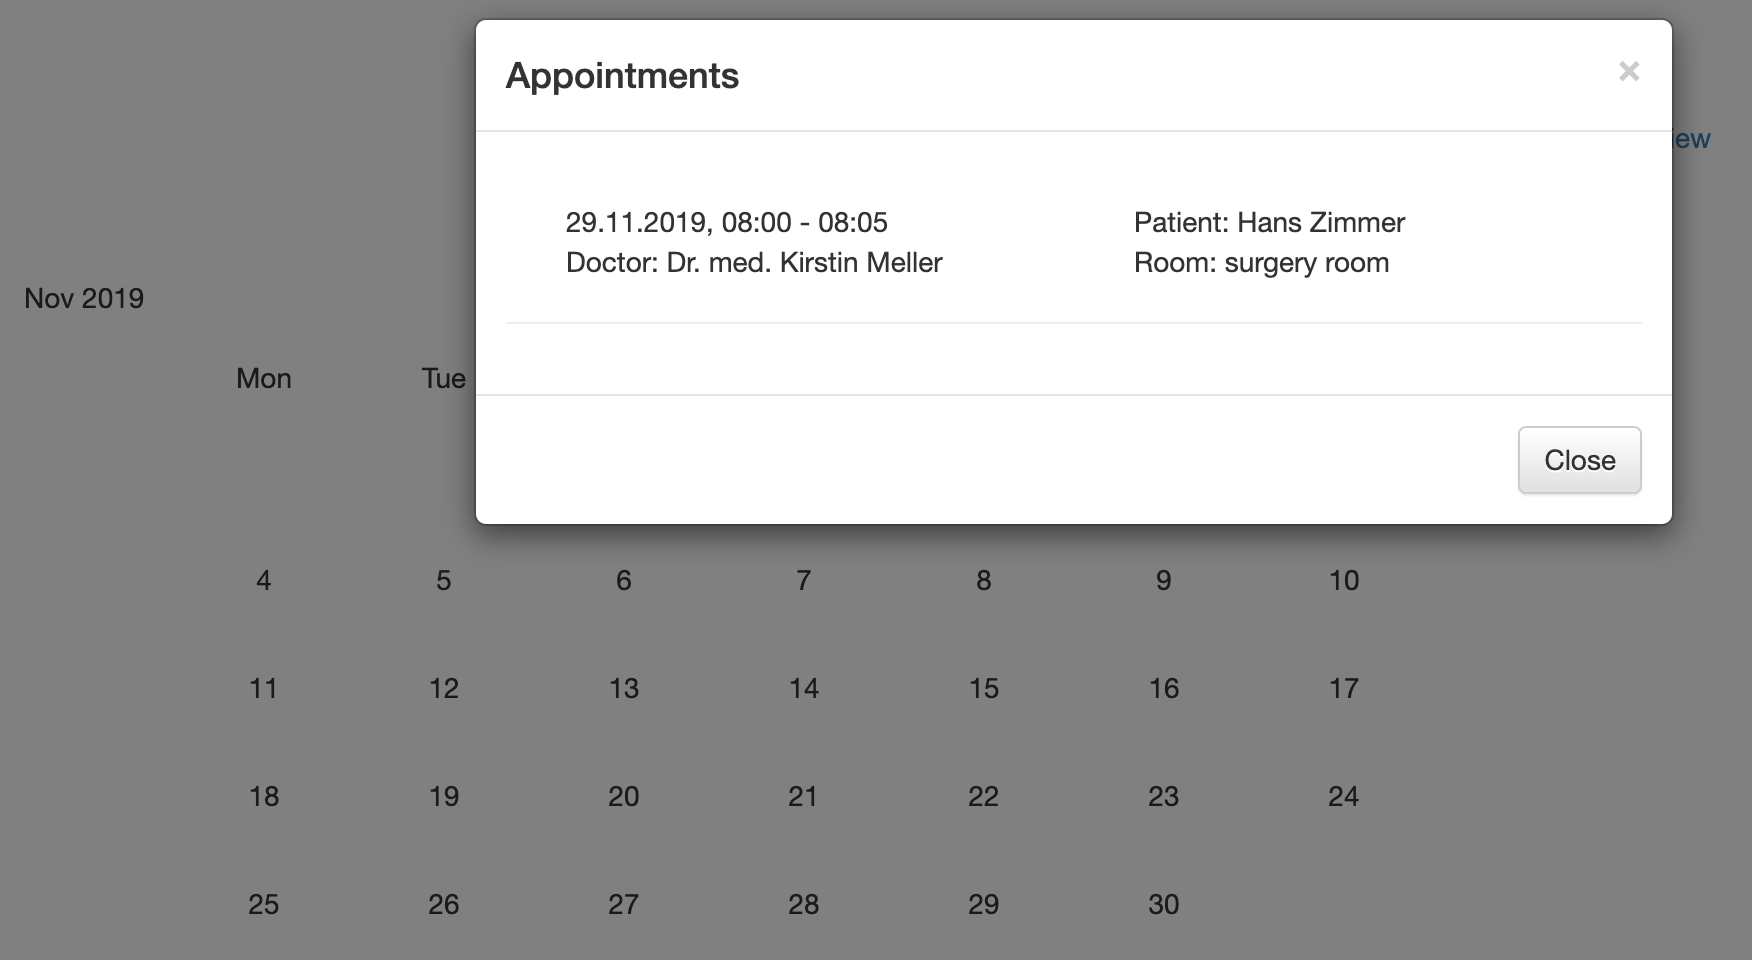
\includegraphics[width=0.8\textwidth]{../figures/screenshots/rewamp-prototype.png}
\caption[Web Migration Prototype Screenshot]{Web Migration Prototype with Web Frontend and \\ Reused Legacy Business Logic in the Backend}\label{fig:awsm.rm.prototype-screenshot}
}
\end{figure}

\vspace{-10pt}
\hypertarget{sec:rwmp.integration}{%
\subsection{Integration with Ongoing Development}\label{sec:rwmp.integration}}
\vspace{10pt}

Integration with ongoing agile software development activities (\cref{c:4} Agile) is an important requirement for all \gls{awsm} methods the neglect of which limits applicability of many \gls{Web Migration} approaches as described in \cref{g:1}.
To avoid this, AWSM:RM method needs to be integrated with ongoing daily development activities of the \gls{isv} on the process and also on the artifacts level.
In \gls{Forward Engineering}, \gls{Rapid Prototyping} is applied early in the development process due to its feedback function and many agile development approaches advocate iterative and incremental \gls{Prototyping} towards an operational prototype  \autocite{Rivero2013MockupDD,Rivero2013,Rivero2014Electra}.
Thus, integration of AWSM:RM is intended in the early stages of a \gls{Web Migration} project.
As the \gls{Rapid Prototyping} paradigm is widely practiced in agile development in industry, AWSM:RM fits nicely in ongoing agile development processes.
The paradigm itself, i.e.~its motivation, value, and high-level process, is known to the developers and does not require further introduction efforts.
The activities required for its three actions can be integrated with ongoing \gls{Forward Engineering} activities in the same context where prototyping  activities for implementation of new functionality or testing new technologies are scheduled.
In the context of the Scrum-based development process in \cref{sec:company-characteristics}, AWSM:RM prototyping activities can be integrated as backlog items in a sprint.
The required effort is limited so that an initial AWSM:RM \gls{web migration prototype} can be achieved within one sprint in parallel to other development activities without blocking too many resources.
On \glspl{artifact} level, the resulting prototype represents a product increment.

\vspace{-10pt}
\hypertarget{sec:mockapi}{%
\subsection{API Prototyping using MockAPI}\label{sec:mockapi}}
\vspace{10pt}

\Glspl{web migration prototype} focus on \gls{ui} and application logic on the client side.
The persistence layer and server side are not the primary concern of a horizontal prototype, because the main motivation is to provide a preview of a potential \webbased version of the \legacy application, not technical feasibility analysis.
However, to achieve a realistic demonstrative prototype in a \gls{Web Migration} context, the client/server communication via a public \gls{api} needs to be represented.
The vast majority (95.8\%) of public \gls{web} \glspl{api} are \gls{rest} \glspl{api} \autocite{Neumann2018PublicApis}.
To solve the technical challenge of providing a prototype with client/server communication via a \gls{rest} \gls{api}, AWSM:RM integrates with an existing method for agile prototyping of \gls{rest} \glspl{api}, MockAPI \autocite{Rivero2013,Rivero2014Electra} and adapts it to \gls{Rapid Web Migration Prototyping} as described in the following.

MockAPI, as shown in \cref{fig:awsm.rm.mockapi.process}, is an agile \gls{mdwe} approach for rapid creation of \glslink{rest}{RESTful} \gls{api} prototypes based on the annotation of \emph{user interface mockups}.
These visual sketches of an envisioned user interface are annotated with \emph{tags} according to the \emph{domain-specific language} (DSL) defined in the MockAPI \gls{metamodel} \autocite{Rivero2013} and its extended version, ELECTRA \autocite{Rivero2014Electra} supported by a \glslink{web}{Web}-based tagging tool\footnote{\url{http://agilemdd.lifia.info.unlp.edu.ar/mockapi/} Retrieved: 6.12.2019}.
The DSL allows to specify the data model in terms of data objects and \gls{cruds} operations, as well as additional constraints and filters.
Based on the specifications in tags, a running \glslink{rest}{RESTful} \gls{api} prototype is then generated for different backends like WebComposition/DataGridService \autocite{Chudnovskyy2010DGS} or node.js.
\begin{figure}[h!]
\hypertarget{fig:awsm.rm.mockapi.process}{%
\centering
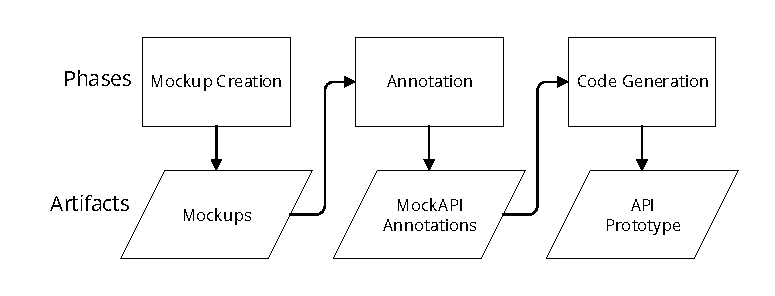
\includegraphics[width=0.85\textwidth]{../figures/mockapi-flowchart.pdf}
\caption{MockAPI Process Flowchart}\label{fig:awsm.rm.mockapi.process}
}
\end{figure}


Integration of AWSM:RM with MockAPI on process level is achieved by following the MockAPI process for action 3 in \cref{fig:awsm.rm.overview}.
Integration on \glspl{artifact} level is achieved by using screenshots of \glslink{Legacy System}{legacy} \glspl{ui} \(u\) instead of \gls{ui} mockups as input for MockAPI.
As described in \cref{sec:formalisms.ls}, these visual \glspl{artifact} can be retrieved from the executables \(E\) of \gls{Legacy System} \(\mathfrak{L}\).
As MockAPI was designed to support different levels of mockups, hand-drawn sketches, as well as digital mockups, created using tools like balsamiq\footnote{\url{https://balsamiq.com/} Retrieved: 6.12.2019}, \glslink{Legacy System}{legacy} \gls{ui} screenshots and mockups can be used interchangeably.
\Cref{fig:mockapi-screenshot} shows the annotation of a screenshot from a \glslink{Legacy System}{legacy} desktop application user interface in the MockAPI editor.

\begin{figure}[h!]
\hypertarget{fig:mockapi-screenshot}{%
\centering
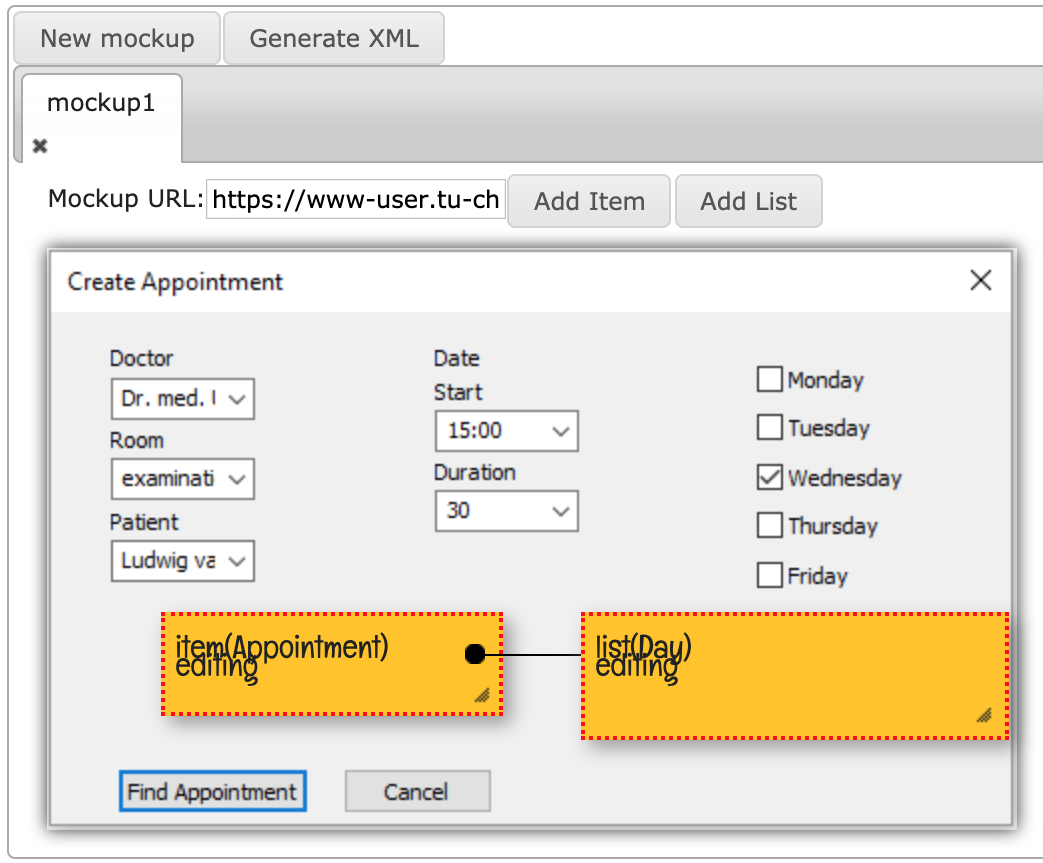
\includegraphics[width=0.85\textwidth]{../figures/screenshots/mockapi2.png}
\caption{Applying MockAPI to a Legacy Desktop User Interface Screenshot}\label{fig:mockapi-screenshot}
}
\end{figure}

\vspace{-15pt}
\hypertarget{sec:rewamp}{%
\section{Reuse of Business Logic}\label{sec:rewamp}}
\vspace{15pt}

To achieve the rapidness of the \gls{Rapid Web Migration Prototyping} with limited resources and to make use of the available expertise of \gls{isv} staff according to \cref{ro:2}, this section describes a technique for Business Logic reuse in \gls{Rapid Web Migration Prototyping}.
Its focus on rapidness provides the second part of the answer to AWSM:RM RQ2.
Due to the horizontal nature of AWSM:RM prototypes, the focus is on the reuse of behavioral business logic (BBL) on the higher layers of \gls{ui} and application logic, similar to the controller layer in an \gls{mvc} architecture.

Reuse of business logic in the approaches assessed in \cref{sec:approaches} has been achieved through \gls{Encapsulation} -- with the shortcomings with regard to representativeness for user interaction with a real \gls{Web Application} as outlined in \cref{sec:sota.discussion} -- or through \gls{Transformation} approaches for the server side.
Client-side reuse of business logic, in contrast, has not received much attention.

\Cref{sec:wmst} assesses suitable technologies for Client-side reuse of business logic, \cref{sec:rewamp.wasm} outlines the reuse technique of AWSM:RM, and \cref{sec:rewamp.implementation} presents the supporting toolchain and \cref{sec:rwmpa} describes a guided prototyping assistance facilitating execution of the technique on the toolchain.

\vspace{-10pt}
\hypertarget{sec:wmst}{%
\subsection[Web Migration Support Technology Assessment]{Assessment of Web Migration Support Technologies}\label{sec:wmst}}
\vspace{10pt}

Recently, a group of technologies that allow for the execution of \glslink{Legacy System}{legacy} code on the client side, in a \gls{web} browser, became available.
We refer to these technologies as \glspl{wmst}, because they can be used as a basis for client-side migration of \glslink{Legacy System}{legacy} code to the \gls{web}.
To assess potential \glspl{wmst}, a comparative experiment was conducted based on a medical appointment scheduling scenario application with the characteristics described in \cref{tbl:legacy_characteristics}.
As shown in \cref{tbl:wmst}, we consider seven candidate \glspl{wmst} that allow executing \glslink{Legacy System}{legacy} C/\cpp code in the browser.
They can be grouped into compilers producing JavaScript, runtimes, browser plugins, and assembly languages.

\vspace{15pt}
\begin{longtable}[]{@{}ll@{}}
\caption[WMST Groups and Implementations]{Web Migration Support Technology Groups and Implementations\label{tbl:wmst}}\tabularnewline
\toprule
Group & Technology\tabularnewline
\midrule
\endfirsthead
\toprule
Group & Technology\tabularnewline
\midrule
\endhead
Compilers producing JavaScript & emscripten \autocite{Zakai2011Emscripten}\tabularnewline
& cheerp\footnote{\url{http://www.leaningtech.com/cheerp/} Retrieved: 6.12.2019}\tabularnewline
Runtimes & Google Native Client\footnote{\url{https://developer.chrome.com/native-client} Retrieved: 6.12.2019}\tabularnewline
Browser Plugin \glspl{api} & NPAPI\footnote{\url{https://developer.mozilla.org/en-US/docs/Plugins/Guide} Retrieved: 6.12.2019}\tabularnewline
& PPAPI\footnote{\url{https://developer.chrome.com/native-client/pepper\_stable} Retrieved: 6.12.2019}\tabularnewline
& js-ctypes\footnote{\url{https://developer.mozilla.org/en-US/docs/Mozilla/js-ctypes} Retrieved: 6.12.2019}\tabularnewline
Assembly Languages & WebAssembly \autocite{W3C2018WebAssembly}\tabularnewline
\bottomrule
\end{longtable}

Following the assessment process in \cref{fig:awsm.rm.rewamp.asessment}, candidate technologies that had not reached the end of support were applied for rapid migration prototyping of the scenario application.
\begin{figure}[h!]
\hypertarget{fig:awsm.rm.rewamp.asessment}{%
\centering
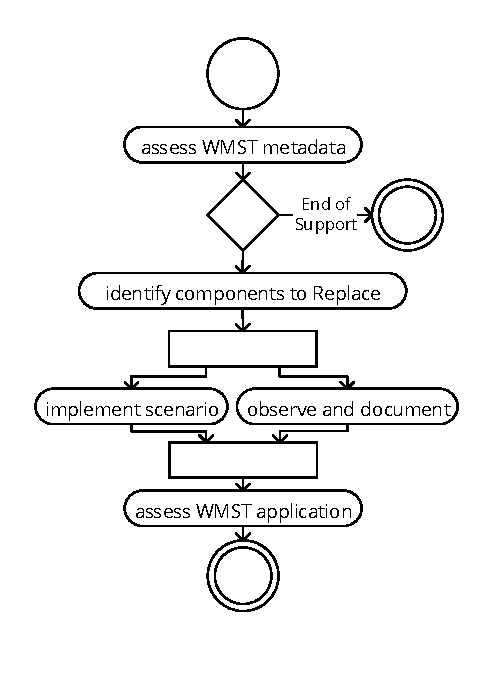
\includegraphics[width=0.4\textwidth]{../figures/rewamp/wmst-assessment.pdf}
\caption[WMST Assessment Process]{Web Migration Technology Assessment Process}\label{fig:awsm.rm.rewamp.asessment}
}
\end{figure}

\pagebreak
The observations provided input for the following five assessment parameters:

\begin{itemize}
\tightlist
\item
  Migration effort
\item
  Limitations
\item
  Platform and OS support
\item
  Currentness of the technology
\item
  Prevalence and supporting partners
\end{itemize}

According to our experiment, WebAssembly (\gls{wasm}) is the most promising \gls{wmst}.
\emph{\gls{wasm}} \autocite{W3C2018WebAssembly} is an open \gls{web} standard (cf.~principle \cref{p:1}) currently designed by the \gls{w3c} WebAssembly Community Group as a format for compilation to the \gls{web} aiming at portability and size- and load-time-efficiency.
The Community Group includes all major browser-developing companies: Google, Mozilla, Apple, and Microsoft.
\gls{wasm} combines the experience from previous work on emscripten and Native Client.
It defines both a binary format optimized for fast execution and a textual format for pretty-printing for human source readers.
Conversion between the two is possible using the WebAssembly Binary Toolkit.
Using parts of the emscripten compiler toolchain, C/\cpp code can be compiled to \gls{wasm} instead of asm.js\footnote{\url{http://asmjs.org/spec/latest} Retrieved: 6.12.2019}.
\gls{wasm} supports dynamic linking for loading DLL dependencies at runtime.
\gls{wasm} has reached the WebAssembly Consensus milestone\footnote{\url{https://webassembly.org/roadmap/} Retrieved: 27.11.2019} with implementation of version 1.0 available in all major browsers.
\Cref{fig:awsm.rm.wasm} shows an overview of \gls{wasm}.

In the experiment, \gls{wasm} showed the fewest limitations, is compatible with all major platforms, is the most current and actively developed technology, and sees comprehensive support from major companies due to being an open standard.
Thus, AWSM:RM realizes client-side reuse of business logic in action 1 based on \gls{wasm}, as described in the next subsection.

\begin{figure}[h!]
\hypertarget{fig:awsm.rm.wasm}{%
\centering
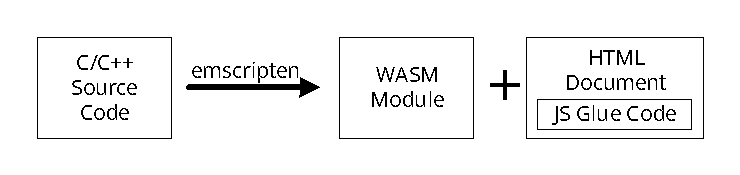
\includegraphics[width=0.99\textwidth]{../figures/rewamp/wasm.pdf}
\caption[WebAssembly Overview]{WebAssembly Overview\footnotemark{}}\label{fig:awsm.rm.wasm}
}
\end{figure}
\footnotetext{adapted from \url{https://developer.mozilla.org/en-US/docs/WebAssembly/Concepts}}

%\pagebreak
\vspace{-10pt}
\hypertarget{sec:rewamp.wasm}{%
\subsection{Rapid Web Migration Prototyping leveraging \\ WebAssembly}\label{sec:rewamp.wasm}}
\vspace{10pt}

\glsunset{rewamp}
\gls{rewamp} \autocite{Heil2018ReWaMP} specifies a process and toolchain for \gls{Rapid Web Migration Prototyping} enabled through client-side reuse of business logic leveraging \gls{wasm}.
This section provides an overview of the architecture of \gls{rewamp} prototypes, shown in \cref{fig:awsm.rm.rewamp.architecture}, and the  process model of \gls{rewamp}, shown in \cref{fig:awsm.rm.rewamp.process}.
The implementation of this process, the supporting toolchain, and the guided \gls{Prototyping} assistance system are described in \cref{sec:rewamp.implementation}.
\begin{figure}[h!]
\hypertarget{fig:awsm.rm.rewamp.architecture}{%
\centering
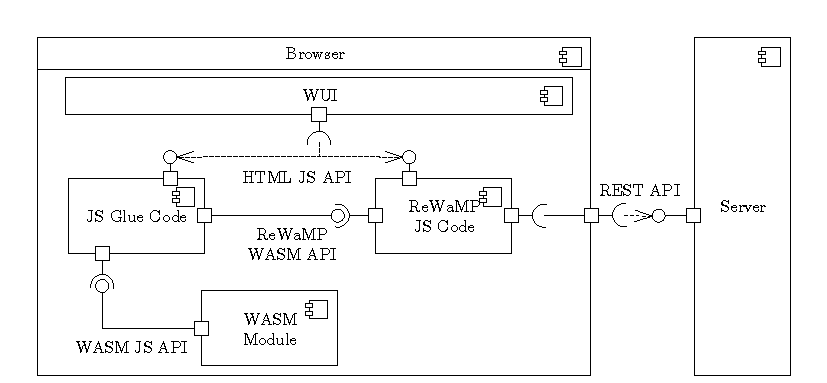
\includegraphics[width=0.9\textwidth]{../figures/rewamp/rewamp-prototype-architecture.pdf}
\caption[Architecture of ReWaMP Prototypes]{Architecture of ReWaMP Prototypes \\\autocite[adapted from][]{Heil2018ReWaMP}}\label{fig:awsm.rm.rewamp.architecture}
}
\end{figure}

\vspace{-15pt}
One \gls{rewamp} prototype is created per user interface \(u \in U\).
\gls{rewamp} prototypes \autocite{Heil2018ReWaMP} consist of the following components: The \emph{\gls{wui}} is a set of \gls{html}/\gls{css} definitions of layout and content structure as created in action 2 of \cref{fig:awsm.rm.overview}.
The \emph{\gls{wasm} Module} is created through the compilation of the \glslink{Legacy System}{legacy} business logic to \gls{wasm}, as shown in \cref{fig:awsm.rm.wasm}.
For each \glslink{Legacy System}{legacy} user interface, the corresponding \gls{wasm} Module contains all \gls{ui} functionality and semantics.
For communication with other components, it is bound to the JS glue code.
The \emph{JS Glue Code} is created during the compilation of \glslink{Legacy System}{legacy} code to \gls{wasm} by the emscripten compiler.
It realizes the \emph{JS \gls{api}} of \gls{wasm}, providing standard functionalities like memory management and serialization of strings for message exchange.
The \emph{\gls{rewamp} JS Code} contains infrastructure for communication with the server and abstraction of the generated \gls{wui}.
Thus, it provides Web-Migration-Prototyping-specific \gls{api} extensions for the JS \gls{api} of \gls{wasm} required to control the behavior from \glslink{Legacy System}{legacy} code compiled to \gls{wasm}.

\begin{figure}[h!]
\hypertarget{fig:awsm.rm.rewamp.process}{%
\centering
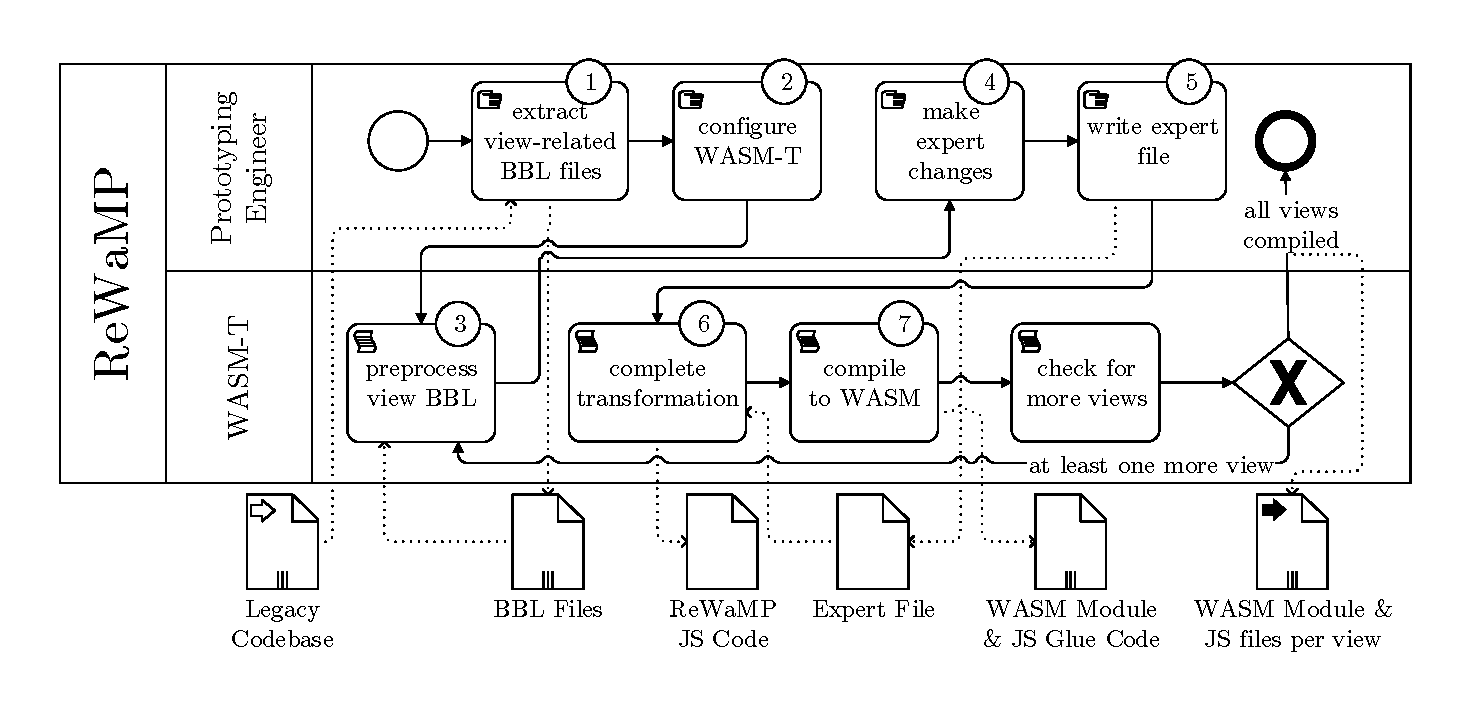
\includegraphics[width=0.99\textwidth]{../figures/rewamp/BPMN_RWMP.pdf}
\caption[ReWaMP Process]{ReWaMP Process \autocite[adapted from][]{Heil2018ReWaMP}}\label{fig:awsm.rm.rewamp.process}
}
\end{figure}

The \gls{rewamp} process \autocite{Heil2018ReWaMP} in \cref{fig:awsm.rm.rewamp.process} produces a \gls{rewamp} prototype by creating the \gls{wasm} Module, JS Glue Code and \gls{rewamp} JS Code for each selected user interface \(u\in U\) -- in the following these top-level \gls{ui} container elements without parents are referred to as \emph{view}, as they correspond to views in the \gls{mvc} pattern.
This is done by extraction of relevant information from the \glslink{Legacy System}{legacy} codebase \(B\), \gls{Transformation} into a \gls{wasm}-compilable version, and compilation to the \gls{wasm} target using emscripten.
To support the rapid creation of \gls{wasm} Modules, the \emph{\gls{wasmt}} provides infrastructure for \cpp -codebases using \gls{mfc} as in the scenario in \cref{sec:scenario-code}.
The responsibilities of the Prototyping Engineer and the WASM Transformator are represented as separate lanes in \cref{fig:awsm.rm.rewamp.process}.

The Prototyping Engineer (1) extracts the source files \(f \in B_u, B_u \subset B\) containing view-related behavioral business logic from the \glslink{Legacy System}{legacy} codebase \(B\), and (2) provides the WASM Transformator with the file location and the main BBL file \(f^* \in B_u\) per view.
Like main functions in \cpp, \emph{main BBL files} \(f^*\) are those files that directly interact with the view \(u\), defining event handlers for \gls{ui} elements.
\gls{wasmt} transforms the extracted \glslink{Legacy System}{legacy} code to make it compilable with WebAssembly.
It uses a semi-automatic process since automated semantic analysis of source code is complex, and the behavioral business logic in \(f_i \in B_u\) can reference dependencies \(dep_j \in Dep\), i.e.~\(\underline D_{i,j} = 1\), which are not available for compilation because they are binaries (\gls{kdm}: \emph{BinaryFile}).
In (3), the WASM Transformator pre-processes the behavioral business logic by deleting/rewriting \gls{gui} framework-specific segments \(s_{fs} \in f \) and extracting \gls{ui} coupling information for introducing the \gls{web} \gls{ui}.

Then, the Prototyping Engineer re-engineers segments \(s^* \in f\) which \gls{wasmt} was not able to transform, either through \emph{expert changes} in situ (4) or within a separate \emph{expert file} (5).
Expert changes replace or remove complex constructs to resolve missing dependencies.
The expert file contains missing declarations and definitions of code items (\gls{kdm}: \emph{CodeItem}) such as classes, variables, and functions.

The required information can be found in the related BBL files \(f\in B_u\) from step 1.
The Prototyping Engineer \emph{mocks}\footnote{cf.~\emph{mock object} \autocite{ISO/IEEE24765Vocabulary}} classes and functions, as the classes require only DTO-like (data transfer object) versions, and the bodies of server-side functions are filled by \gls{wasmt} in (6).
\gls{wasmt} completes the \gls{Transformation} (6) through the generation of function bodies in the expert files and \gls{rewamp} JS code for communication support between \gls{wasm} and \gls{wui} and \gls{wasm} and the server side, respectively.
Finally, the code is compiled to \gls{wasm} (7).

\pagebreak
%\vspace{-10pt}
\hypertarget{sec:rewamp.implementation}{%
\subsection{Rapid Web Migration Prototyping Toolchain}\label{sec:rewamp.implementation}}
\vspace{10pt}

Implementation of \gls{rewamp} based on \gls{wasm} introduces four technical challenges, which are briefly outlined in the following.
\emph{\gls{wasm} data serialization}, owing to its focus on accelerating computation-intensive \glspl{Web Application} like in-browser games, is a challenge since \gls{wasm} only supports 32 and 64-bit integers and floats.
Passing more complex data like arrays or objects into and out of the \gls{wasm} Module must be implemented via memory allocation (heap-based) and passing of pointers via JS Glue Code.
For strings, JS Glue Code provides a UTF \gls{api}.
\gls{rewamp} uses this \gls{api} to serialize any non-numerical data to UTF strings in JSON.
\emph{Client/Server Communication} between \gls{wasm} Module and \gls{rest} \gls{api} is implemented via the \gls{rewamp} JS Code transparently: it handles the data serialization, communication via AJAX, and object instantiations based on responses to the \gls{wasm} Module as synchronous method invocation.
\emph{DOM Access} from \gls{wasm} Module for reading input data from the \gls{wui} and changing the \gls{ui} state is supported by \gls{rewamp} JS Code similar to the Client/Server communication mechanism.
\emph{\gls{ui} event handling} is provided by the \gls{rewamp} runtime by forwarding events to automatically exported methods of the \gls{wasm} Module within \gls{rewamp} JS Code.

\begin{figure}[h!]
\hypertarget{fig:awsm.rm.wasmt.architecture}{%
\centering
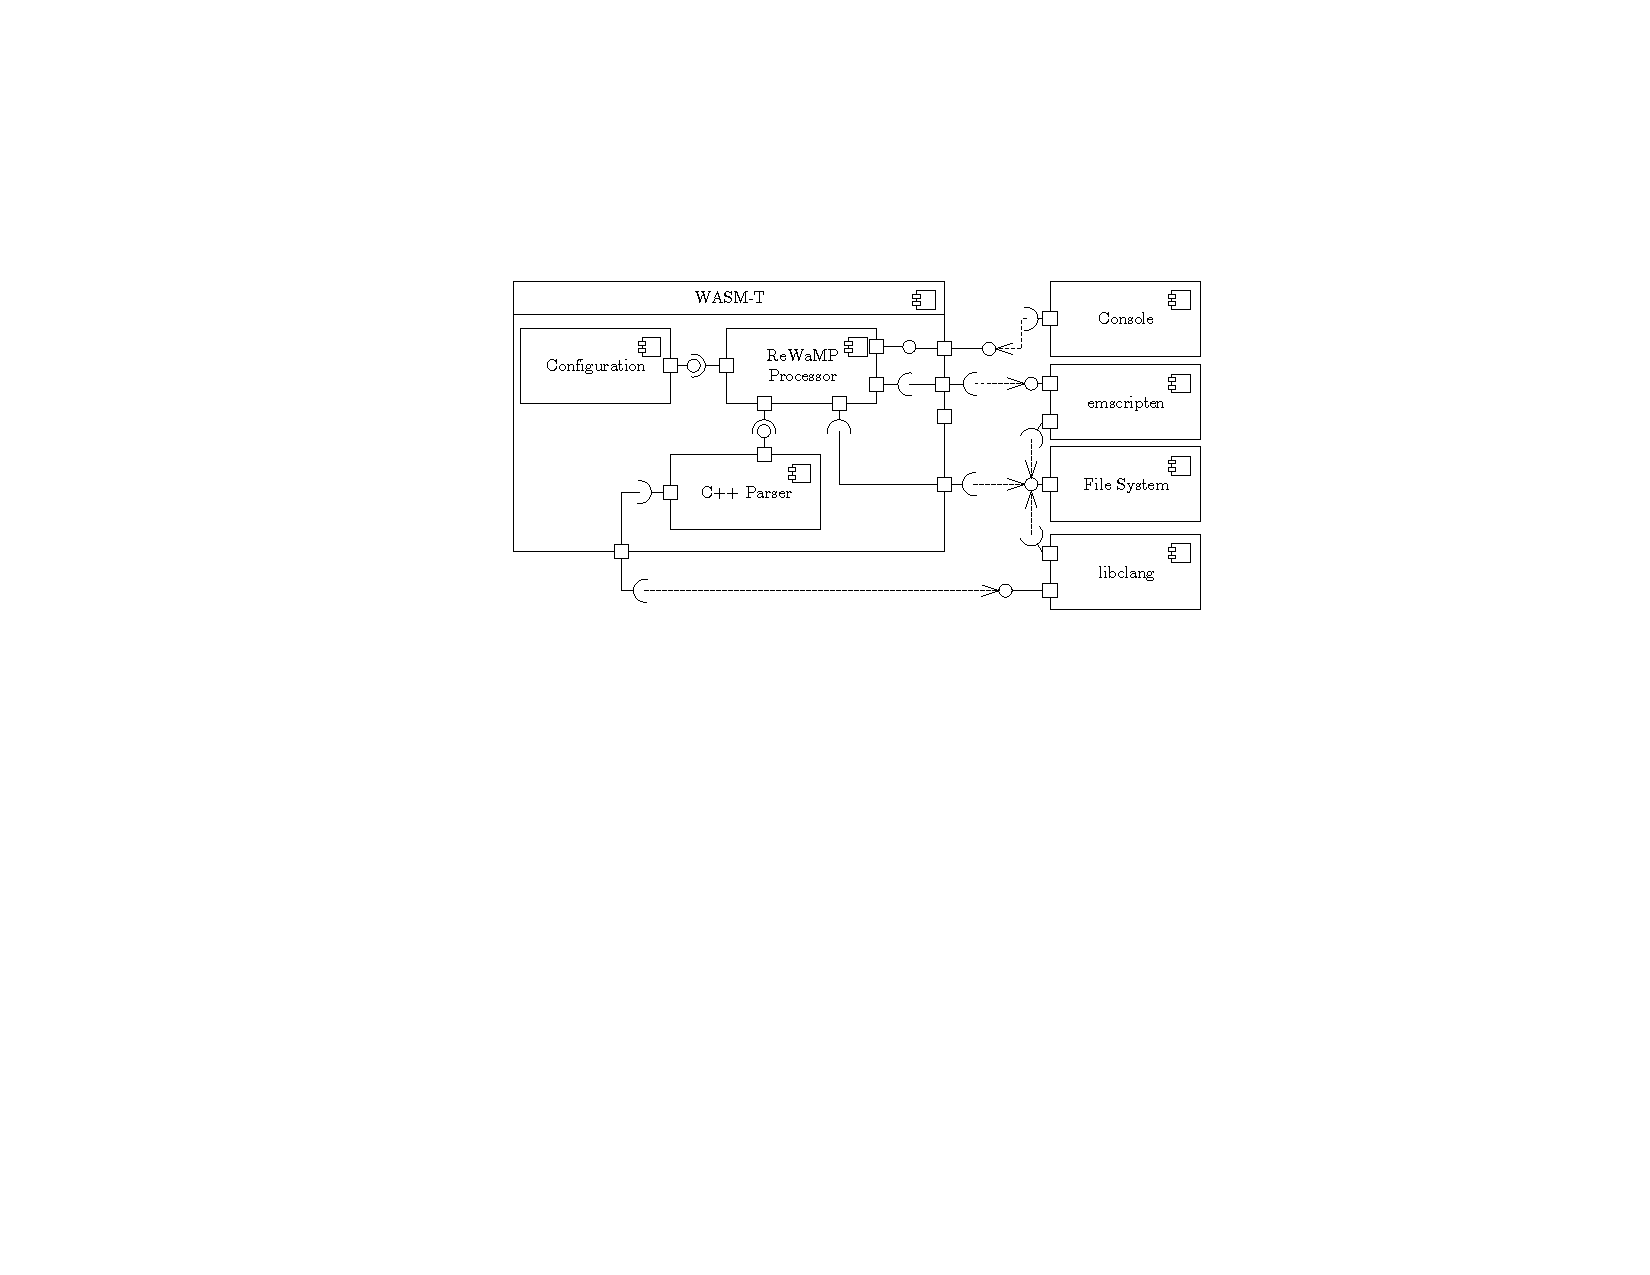
\includegraphics[width=0.9\textwidth]{../figures/awsm-rm-wasmt-architecture.pdf}
\caption{WASM Transformator Architecture}\label{fig:awsm.rm.wasmt.architecture}
}
\end{figure}

\Cref{fig:awsm.rm.wasmt.architecture} shows the architecture of the WASM Transformator, which provides a toolchain supporting the \gls{rewamp} process.
\gls{wasmt} is implemented as command-line tool in python and uses the python bindings of libclang\footnote{\url{https://clang.llvm.org/docs/Tooling.html} Retrieved: 6.12.2019} for parsing the \glslink{Legacy System}{legacy} source code.

The main components are \gls{rewamp} processor and the \cpp parser.
The \emph{configuration} interacts with the Prototyping Engineer as in step 2 in \cref{fig:awsm.rm.rewamp.process} and stores the list of all main and related BBL files and the tool paths of libclang and emscripten.

The \emph{\cpp parser} component parses the codefiles \(f\in B\) using libclang to identify segments \(s \in f\) for \gls{Transformation} and provides a custom interface for the \gls{rewamp} processor.
The clang parser creates an \gls{ast} representation of \(f\), which is traversed to identify segments \(s\) representing program elements (\gls{kdm}: \emph{CodeItem}) like includes, variables, functions, classes, as shown in \cref{fig:rewamp-parser} and provide the \gls{rewamp} processor with this information.

\setlength{\algomargin}{2em} %
\begin{algorithm}
	\DontPrintSemicolon
	\KwIn{Configuration $\textrm{Cfg}$, view behavior files $B_u$ per view $u$}
	\KwOut{ReWaMP runtime for each view $u$}
	\SetKwBlock{Begin}{function}{end function}
	\Begin($\text{ReWaMPProcess} {(} {)}$)
	{
		$B_u = \text{readAllFilesInDir}{(}\textrm{Cfg}.\text{workingDir}{)}$\;
		\ForEach{$f^*$ in $\textrm{Cfg}.\text{mainFiles} $}
		{
			$cursor_{now} = \text{getMainCursor}{(}f^*$ in $\textrm{Cfg}.\text{workingDir},$ True${)}$\;
			$B'_u = \text{getRelatedFiles}{(}cursor_{now},$ $B_u{)}$\;
			$B'_u = \text{editIncludings}{(}cursor_{now},$ $B'_u,$ $\textrm{Cfg}.\text{headers}{)}$\;
			$B'_u,$ $maps = \text{minorChanges}{(}B'_u{)}$\;
			$dir_{rel} = \text{createRelatedDir}{(}f^*{)}$\;
			$cursor_{now} = \text{saveRelFilesGetCursor}{(}f^*$ in $dir_{rel},$ $B'_u{)}$\;
			$B'_u = \text{deleteUnusedParams}{(}cursor_{now},$ $B'_u{)}$\;
			$B'_u,$ $bodies,$ $funcs = \text{editMFCFunctions}{(}cursor_{now},$ $B'_u{)}$\;
			saveRelatedFiles${(}B'_u{)}$\;
			printHints${(}cursor_{now},$ $B'_u{)}$\;
			waitForME${(}{)}$\;
			$B'_u = \text{loadRelatedFiles}{(}{)}$\;
			$cursor_{now} = \text{getMainCursor}{(}f^*$ in $dir_{rel}{)}$\;
			$bodies = \text{buildExpertFunctions}{(}cursor_{now},$ $B'_u,$ $bodies{)}$\;
			$B'_u = \text{addJSONMethods}{(}cursor_{now},$ $B'_u{)}$\;
			$B'_u = \text{processFlags}{(}B'_u{)}$\;
			$cursor_{now} = \text{saveRelFilesGetCursor}{(}f^*$ in $dir_{rel},$ $B'_u{)}$\;
			$embinds,$ $funcs = \text{collectEmbinds}{(}cursor_{now},$ $B'_u,$ $maps,$ $funcs{)}$\;
			$cursor_{now} = \text{saveRelFilesGetCursor}{(}f^*$ in $dir_{rel},$ $B'_u{)}$\;
			$B'_u = \text{addFunctions}{(}cursor_{now},$ $B'_u,$ $funcs{)}$\;
			$cursor_{now} = \text{saveRelFilesGetCursor}{(}f^*$ in $dir_{rel},$ $B'_u{)}$\;
			$B'_u = \text{writeNewBodies}{(}cursor_{now},$ $B'_u,$ $bodies{)}$\;
			$B'_u = \text{addSendStatusFunction}{(}B'_u{)}$\;
			$B'_u = \text{addEmbinds}{(}embinds,$ $B'_u{)}$\;
			saveRelatedFiles${(}B'_u{)}$\;
			copyLibraryFiles${(}dir_{rel}{)}$\;
			addJSInitFunction${(}embinds,$ $maps{)}$\;
			compileFilesToWasm${(}B'_u{)}$\;
		}\label{endfor}
	}
	\caption{ReWaMP Process Algorithm}\label{alg:rwmp}
\end{algorithm}

The \emph{\gls{rewamp} processor} is the core component of \gls{wasmt}, implementing the code \gls{Transformation}.
It is controlled via a console interface and uses the emscripten compiler to compile all related BBL files to the \gls{wasm} Module.
\Cref{alg:rwmp} shows the pseudo code of the algorithmic realization of \gls{wasmt} \gls{Transformation} in the \gls{rewamp} processor.
It implements steps 3 (line 4-12), 6 (line 15-30) and 7 (line 31) of \cref{fig:awsm.rm.rewamp.process}.
\emph{BBL preprocessing} manages the includes in related files \(f \in B_u\) by replacing \gls{gui} framework-specific types, function calls and extracts message maps representing module communication.
Following the manual steps of the Prototyping engineer, for \emph{Tranformation completion} the \gls{rewamp} processor fills function body stubs with generated code for calling functionality on the server side, serialization, and to expose code for the \gls{ui} event handling from JavaScript.
The \gls{wasmt} support of semi-automatic \gls{Transformation} is based on the technical assumptions listed in \cref{tbl:rewamp-assump}.
\Cref{lst:rewampreturns} shows an example of source code generated by the \gls{rewamp} processor.
This code handles the passing of return values between a \legacy function in the \gls{wasm}-compiled \cpp code and JavaScript code.
It is implemented with the \emph{Inline JavaScript} \texttt{EM\_ASM()} method of emscripten.
The example shows the passing of a string through UTF8 serialization, memory allocation, and management of the \gls{wasm} heap using a \texttt{char} array pointer.

\begin{lstlisting}[language=C++, captionpos=t, caption=Example of Code Generated by ReWaMP to Handle Passing of Return Value from Function Call, label=lst:rewampreturns,breaklines=true,postbreak=\mbox{$\hookrightarrow$\space},]
std::string rs = (char *) EM_ASM_INT({
  var data_string = UTF8ToString($0);
  var return_string = send_server_function(data_string);
  var lengthBytes = lengthBytesUTF8(return_string) + 1;
  var stringOnWasmHeap = _malloc(lengthBytes);
  stringToUTF8(return_string, stringOnWasmHeap,
   lengthBytes + 1);
  return stringOnWasmHeap;
}, cha);
\end{lstlisting}

\vspace{-10pt}
\hypertarget{sec:rwmpa}{%
\subsection{Guided Web Migration Prototyping Assistance}\label{sec:rwmpa}}
\vspace{10pt}

To achieve the limited resources expertise constraint of \cref{ro:2}, AWSM:RM provides the \emph{\gls{rwmpa}}, an assistance system that guides Prototyping Engineers through the \gls{rewamp} process, providing an answer to AWSM:RM RQ3.
The need for providing guidance was identified in initial experiments with \gls{rewamp} and its toolchain \gls{wasmt} (cf.~\cref{sec:rewamp.experiment}) due to the complexity of the \gls{rewamp} process and the observed demand for improved tool support compared to the console-based interaction with \gls{wasmt} and external editor-based manual interventions
The resulting guided process is referred to as \emph{\gls{rwmpa} workflow} in the following.
It contains adaptions to the process in \cref{fig:awsm.rm.rewamp.process} based on the feedback from experimentation with \gls{rewamp} to implement the process at a higher level of detail for better usability.
The detailed \gls{rwmpa} workflow is presented in \cref{fig:rwmpa-process}. 
\Cref{tbl:rewamp-rwmpa} shows the mapping between the process introduced in \cref{fig:awsm.rm.rewamp.process} and the tasks of the adapted workflow.
\gls{rwmpa} is implemented as extensible model-driven \gls{Web Application}: the basic workflow was modeled in \gls{bpmn} 2.0 and is instantiated using the Camunda Workflow Engine\footnote{\url{https://camunda.com/products/bpmn-engine/} Retrieved: 6.12.2019} on top of which the \gls{rwmpa} \gls{Web Application} provides a \glslink{web}{Web} user interface guiding the Prototyping Engineer.
In this way, the process can be adapted and extended to specific requirements diverging from the scenario in \cref{sec:scenario} when employed with different \gls{Web Migration} approaches.

\hypertarget{tbl:rewamp-rwmpa}{}
\begin{xltabular}{\linewidth}[hbt]{@{}ll@{}}
\caption[ReWaMP tasks and realization in RWMPA workflow]{\label{tbl:rewamp-rwmpa}ReWaMP tasks and realization in RWMPA workflow.
M and T indicate manual tasks and tasks by WASM-T in ReWaMP, U and S designate user and service tasks in RWMPA}\tabularnewline
\toprule
Original (ReWaMP) process & Guided (RWMPA) workflow\tabularnewline
\midrule
\endfirsthead
\toprule
Original (ReWaMP) process & Guided (RWMPA) workflow\tabularnewline
\midrule
\endhead
1M extract view-related BBL files & 5S find rel. files, 6U select files\tabularnewline
2M configure WASM-T & automatically, not in workflow\tabularnewline
3T preprocess view BBL & 7S preprocess\tabularnewline
4M expert changes & 10U del.
code, 11U repl.
code,\tabularnewline
 & 16U exp.
changes\tabularnewline
5M expert file & 16U expert changes\tabularnewline
6T complete transformation & 17S save\tabularnewline
7T compile to \gls{wasm} & 14S compile to \gls{wasm}\tabularnewline
\bottomrule
\end{xltabular}

\Cref{fig:awsm.rm.rwmpa.screenshot.start} shows a screenshot of the start page of the RWMPA system.
It provides an overview of the entire workflow in BPMN on top and detailed instructions on how to conduct the Prototyping.
The instructions can be re-visited in any step of the guided process.
Additionally, each step displays a similar instruction page explaining the use of the RWMPA tools to the Migration Engineer, including screenshots.

\begin{figure}[h]
\hypertarget{fig:awsm.rm.rwmpa.screenshot.start}{%
\centering
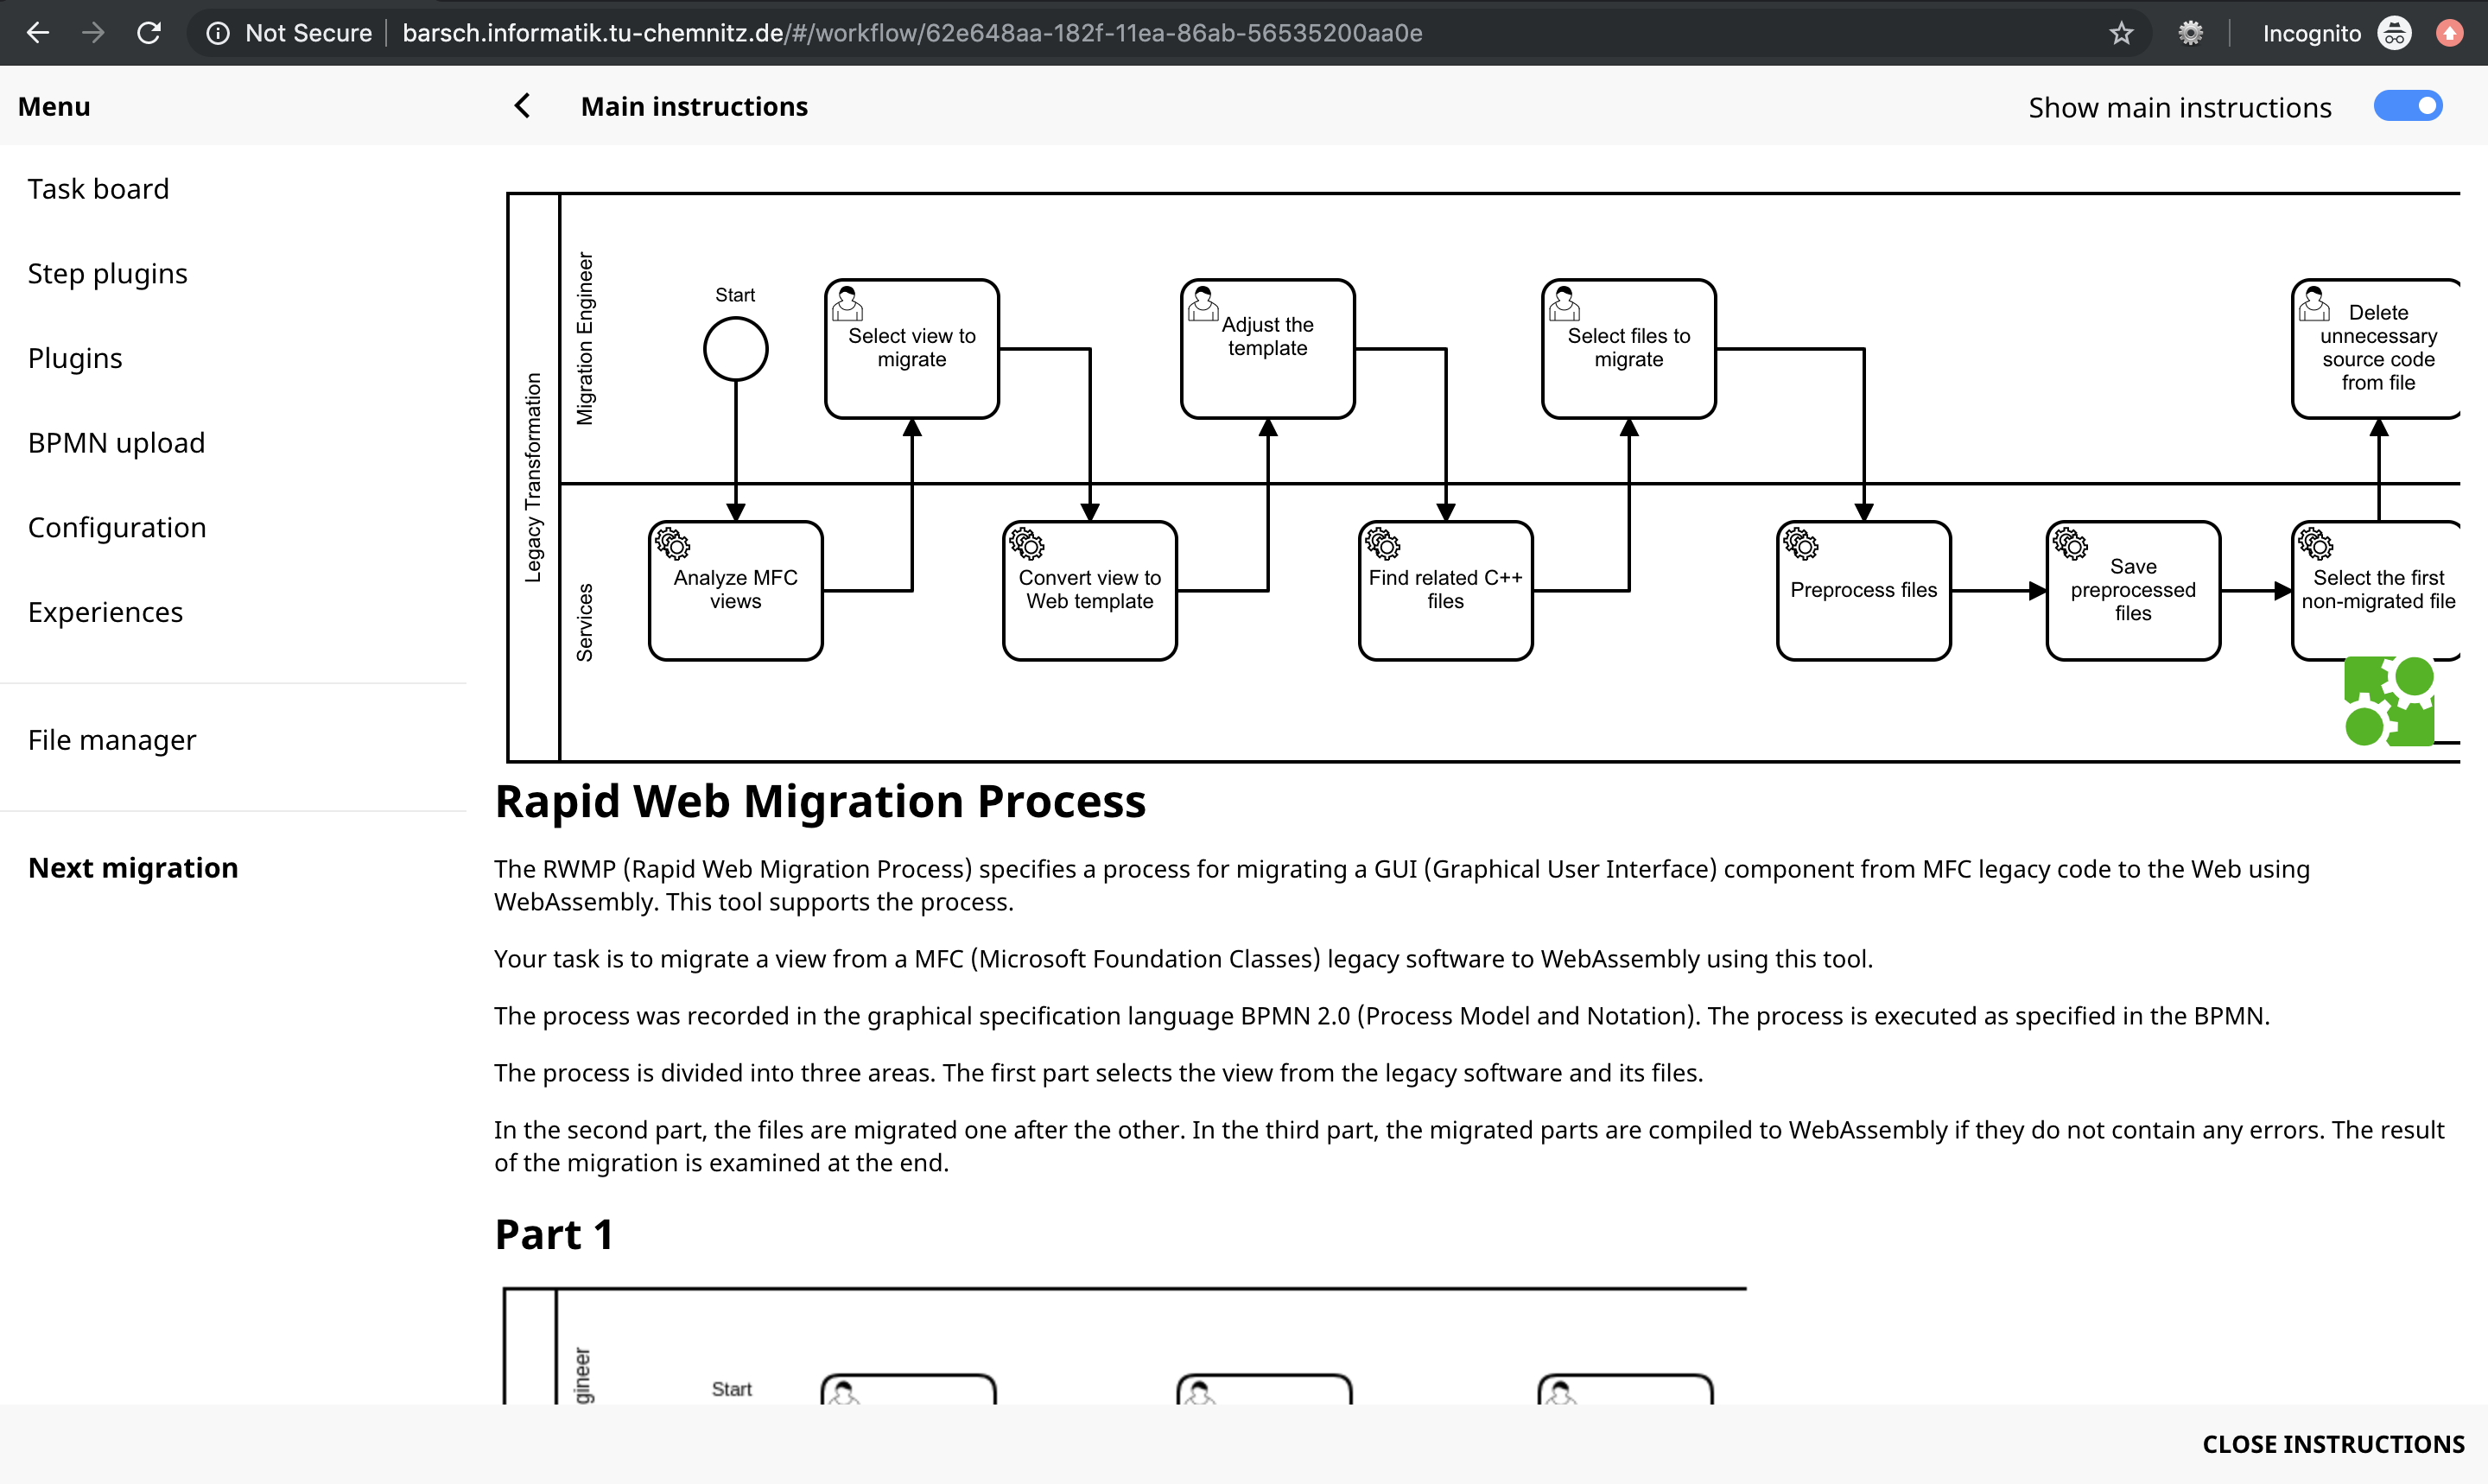
\includegraphics[width=0.99\textwidth]{../figures/screenshots/rwmpa-start.png}
\caption{RWMPA Workflow Start Page explaining Required Steps}\label{fig:awsm.rm.rwmpa.screenshot.start}
}
\end{figure}

As shown in \cref{fig:rwmpa-architecture}, \gls{rwmpa} is designed in a modular style: each step in the workflow is interfaced in the \gls{wui} in detail and in the context of the overall process.
\gls{rwmpa} provides a default implementation for the details of each step (\emph{step worker page}) that displays a description of required activities.
Via its Plugin Service, specific implementations of workflow steps can be registered, consisting of frontend \emph{plugins} and backend \emph{migration services}.
\gls{rwmpa} manages the context of the plugins, e.g.~providing the required input and storing the output artifacts and invokes the plugin implementation when the Prototyping Engineer reaches the corresponding step.
This allows for extension of \gls{rwmpa} with additional automation and with rapid \web migration tools with improved usability.
The \gls{rwmpa} frontend is implemented in TypeScript with Angular-based Ionic\footnote{\url{https://ionicframework.com/} Retrieved: 6.12.2019} 4.
Plugins are compiled to \gls{w3c} WebComponents \autocite{W3C2018WebComponents} for embedding in a step worker page using on the stencil\footnote{\url{https://stenciljs.com/} Retrieved: 6.12.2019} compiler, \gls{rwmpa} migration services are implemented in node.js.

\gls{rwmpa} implements a set of plugins, including file management and source code editing for steps 4 and 5 in \cref{fig:awsm.rm.rewamp.process} with syntax highlighting.
\Cref{fig:awsm.rm.rwmpa.screenshot} shows a merge view of \gls{rwmpa} supporting the Prototyping Engineer to review and accept or reject changes from \gls{wasmt} preprocessing.
The left side shows the code of the original \glslink{Legacy System}{legacy} code; the right side shows the code after preprocessing by the WASM Transformator, which tries to resolve dependencies by adding corresponding includes and adapting the types accordingly.
The Merge View highlights changes which can be accepted or rejected by the Prototyping engineer, and also allows direct editing in the code editor on the right.
\begin{figure}[h]
\hypertarget{fig:awsm.rm.rwmpa.screenshot}{%
\centering
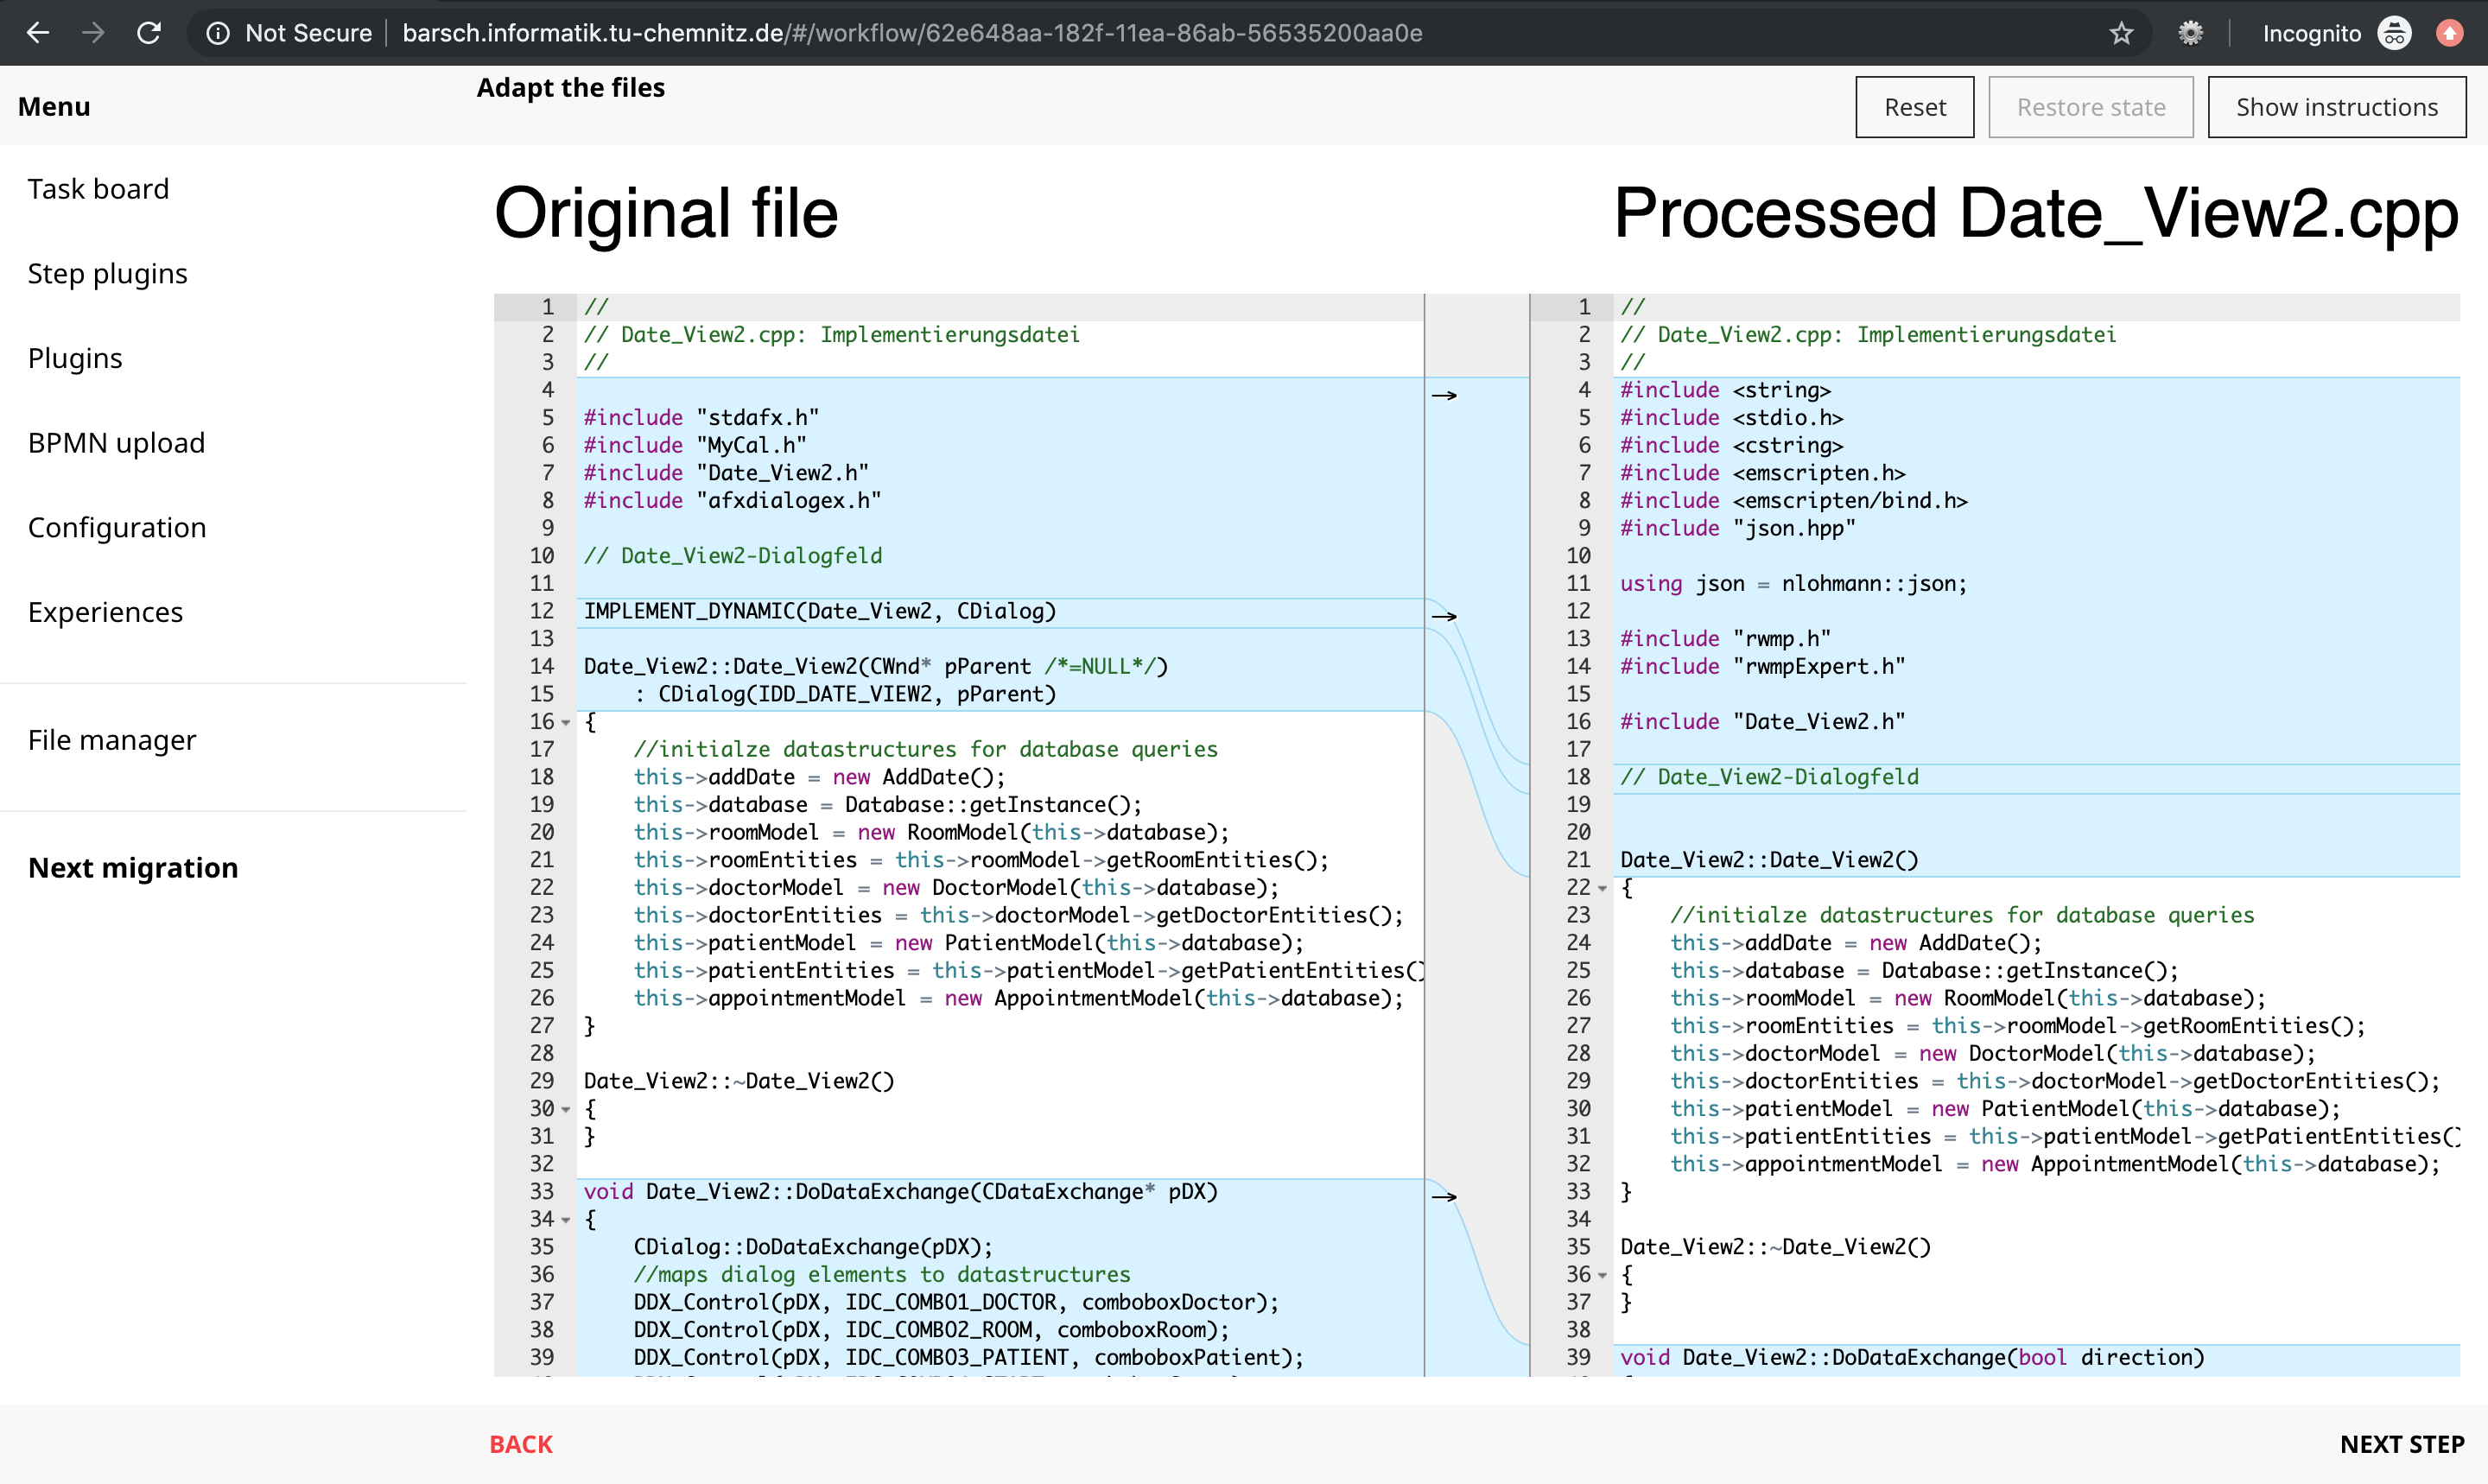
\includegraphics[width=0.99\textwidth]{../figures/screenshots/rwmpa-review-preprocessing.png}
\caption{RWMPA Step Worker Page Example: Merge View}\label{fig:awsm.rm.rwmpa.screenshot}
}
\end{figure}

\vspace{-15pt}
\hypertarget{sec:uitransformation}{%
\section{User Interface Transformation}\label{sec:uitransformation}}
\vspace{15pt}
To demonstrate a prototypical \glslink{web}{Web}-based version of the \gls{Legacy System} for \cref{ro:2}, a \glslink{web}{Web} user interface similar to the \legacy user interface needs to be created.
AWSM:RM action 2 in \cref{fig:awsm.rm.overview} defines this creation as semi-automatic \gls{Transformation} of the \gls{Legacy System} to meet the resources and expertise constraint of \cref{ro:2} and answering the demand for automation of AWSM:RMRQ3.
This section presents the realization of the user interface transformation of action 2.
\Cref{sec:uitransformation.problem} outlines the conceptual problem of mapping \legacy to \gls{web} layouts, \cref{sec:uitransformation.evolutionary} defines a process for computing the mapping based on evolutionary optimization, and \cref{sec:uitransformation.tool} describes the implementation of this process in the UI Transformer tool.

\vspace{-10pt}
\hypertarget{sec:uitransformation.problem}{%
\subsection{Mapping Legacy to Web Layouts}\label{sec:uitransformation.problem}}
\vspace{10pt}

\gls{Transformation} of a \glslink{Legacy System}{legacy} user interface \(u\) to a \glslink{web}{Web}-based version is difficult due to conceptual differences in the user interface layouts.
\glslink{Legacy System}{Legacy} desktop user interfaces are built using a variety of heterogeneous frameworks and a \legacy layout \(l_{legacy}\) is described as  pixel-based mapping of controls \(c\) into two-dimensional cartesian space as defined in the formalism in \cref{sec:ui-formalism}. 
Modern \gls{web} user interfaces adhere to the \emph{Responsive Web Design} paradigm \autocite{Marcotte2010Responsive,Nebeling2013Responsive}: they dynamically adapt to different viewing environments, i.e.~aspect ratios, resolutions, screen sizes etc.
This is realized through fluid grids, defining the \gls{wui} as \emph{grid layout} \(l_{grid}\) consisting of \emph{rows} and \emph{columns}.
Implementations of grid layouts are based on popular frameworks like bootstrap\footnote{\url{https://getbootstrap.com/} Retrieved: 6.12.2019} or on the \gls{css} Grid Layout standard \autocite{W3C2017CSSGrid}.
\Cref{fig:uitransformer.layout} represents the two different layout paradigms, pixel-based on the left side and grid layout on the right side, which need to be mapped for the \gls{Transformation}.

\begin{figure}[h!]
\centering

\subfloat[Legacy Pixel-based Layout]{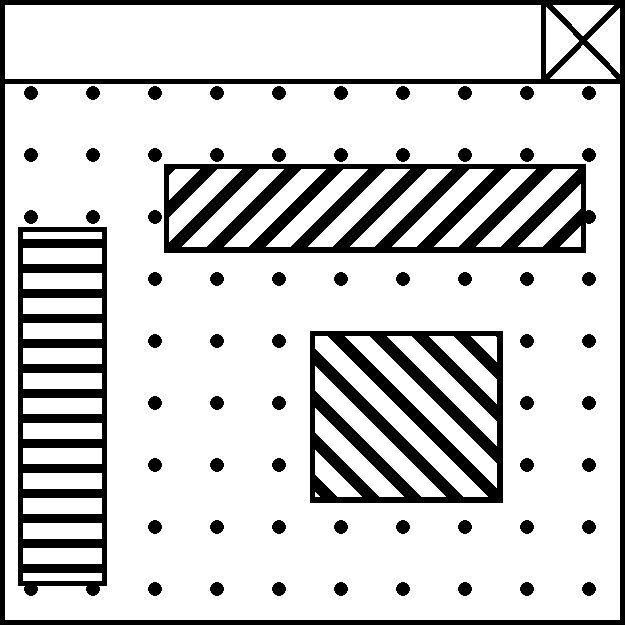
\includegraphics[width=0.35\textwidth]{../figures/uitransformer/legacy.pdf}\label{fig:uitransformer.layout-a}}
\qquad
\subfloat[Transformed Grid Layout]{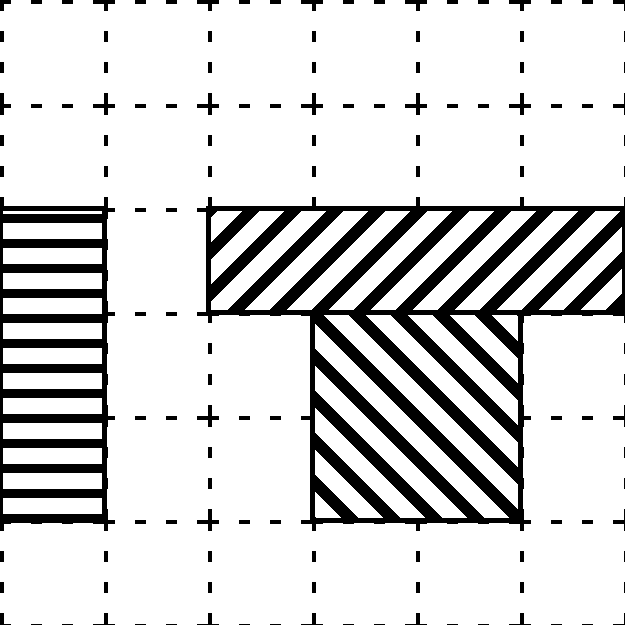
\includegraphics[width=0.35\textwidth]{../figures/uitransformer/grid.pdf}\label{uitransformer.layout-b}}

\caption{Layout Transformation: Mapping Pixel-based to Grid Layouts}
\label{fig:uitransformer.layout}
\end{figure}

Thus, realizing action 2 of AWSM:RM as shown in \cref{fig:awsm.rm.overview} requires a mapping from pixel-based to grid layouts.
Finding this mapping is an \emph{optimization problem} with discrete variables: it tries to minimize an \emph{objective function} under a set of \emph{hard and soft constraints}.
The objective function is a similarity measure.
The discrete variables are the possible positions and sizes in the grid layout, and the constraints represent the nature of grid layouts, as outlined in the following.
\vspace{-8pt}

Compared to pixel-based layouts, the rows and columns of grid layouts divide the continuous Euclidean plane into discrete \emph{cells}, thus imposing constraints on the placement of controls.
A grid layout can have an infinite number of rows, but it has a fixed number of columns \(n_{grid} \in \mathbb{N}^+\), distributed equally within the width of the viewport \(w_{viewport}\).
A control \(c\) is assigned to one or more cells.

The bounding box \(b = (x,y,w,h)\) defined in \cref{eq:bounding-box} of a control \(c\) in \(l_{grid}\) reflects these grid constraints as follows:

\begin{equation}
\begin{aligned}
x &\in \bigg\{i \cdot \frac{w_{viewport}}{n_{grid}} \text{ }\bigg |\text{ } 0 \leq i < n_{grid} \bigg\} & y &\in \{j \cdot h_{row} \text{ }|\text{ } j \in \mathbb{N}_0 \} \\
w &\in \bigg\{k \cdot \frac{w_{viewport}}{n_{grid}} \text{ }\bigg |\text{ } 1 \leq i < n_{grid} - x \bigg\} & h &\in \{l \cdot h_{row} \text{ }|\text{ } l \in \mathbb{N} \}
\end{aligned}
\end{equation}

Valid bounding boxes have horizontal positions \(x\) that are a multiple of the column width \(\frac{w_{viewport}}{n_{grid}}\), vertical positions \(y\) that are a multiple of the row height \(h_{row}\), a width \(w\) as multiple of column width that ensures that \(c\) is assigned to at least one column and that prevents a row overflow by ensuring the constraint \(x + w \leq w_{viewport}\) and a height \(h\) a multiple of \(h_{row}\) that ensures that \(c\) is assigned to at least one row.
\(L_{grid}\) is the set of all valid grid layouts.
%The grid constraints define a mapping from a pixel-based onto a grid layout, as the values of indices \(i,j,k,l\) determining the position in the grid allow calculation of the cartesian coordinates and vice versa.

\vspace{-20pt}
\hypertarget{sec:uitransformation.problem}{%
\subsection[User Interface Transformation through\\ Evolutionary Optimisation]{User Interface Transformation through Evolutionary Optimisation}\label{sec:uitransformation.evolutionary}}
\vspace{20pt}

Due to the limited resources in \cref{ro:2}, layout \gls{Transformation} needs to be automated.
This requires solving the optimization problem of mapping a given pixel-based \(l_{legacy}\) to a grid layout \(l_{grid}\) in the constrained grid-cell space through an algorithm.
For AWSM:RM, the optimization is implemented as \emph{evolutionary algorithm} \autocite{Weise2009Optimization}.
\Cref{fig:awsm.rm.uitransformation.process} shows the process of UI Transformation using evolutionary optimization.

\begin{figure}[h!]
\hypertarget{fig:awsm.rm.uitransformation.process}{%
\centering
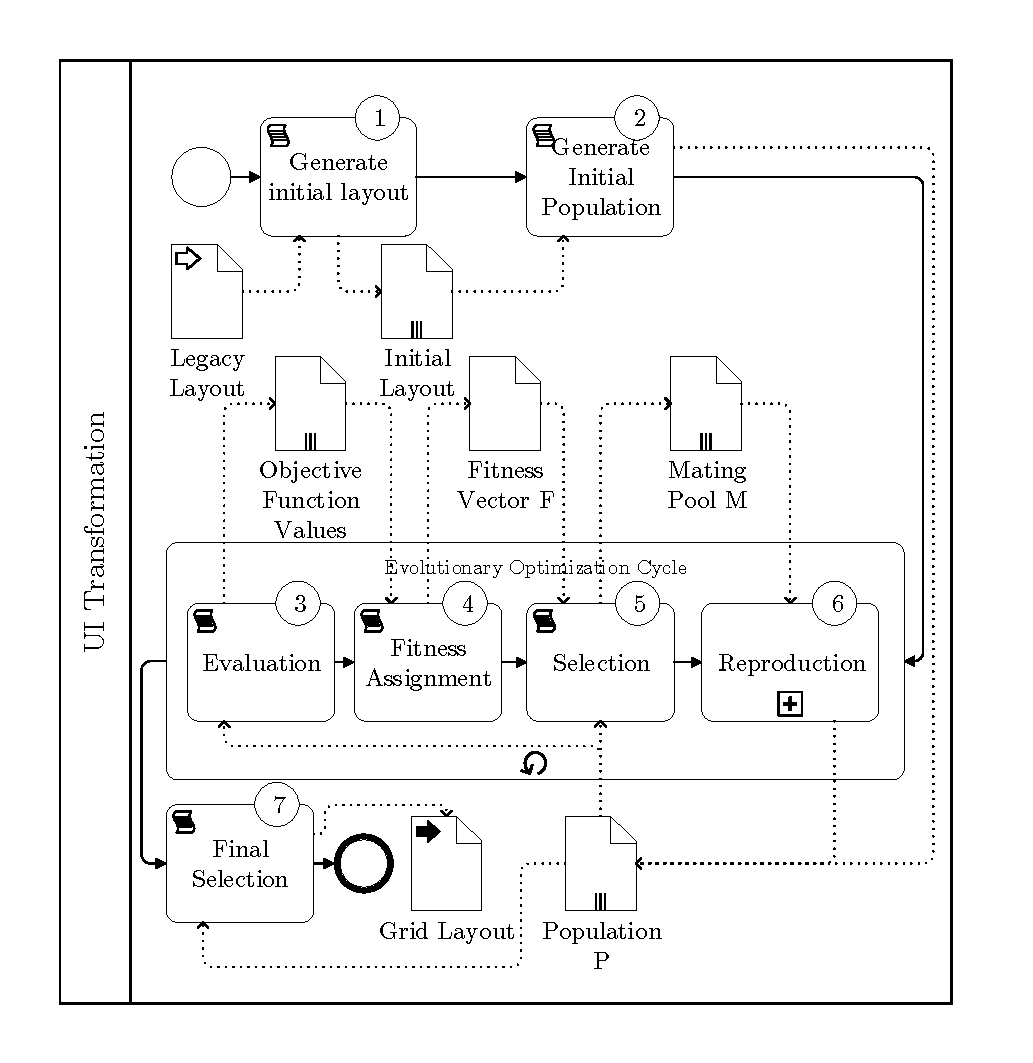
\includegraphics[width=0.85\textwidth]{../figures/awsm-rm-UITransformation-BPMN.pdf}
\caption{UI Transformation Process}\label{fig:awsm.rm.uitransformation.process}
}
\end{figure}

The algorithm tries to optimize the characteristics by creating new \emph{individuals} -- grid layouts -- from existing ones.
Based on an \emph{initial population} \(P_0 \subset L_{grid}\), a cycle of \emph{evaluation}, \emph{fitness assignment}, \emph{selection}, and \emph{reproduction} is repeated, incrementally creating new populations of grid layouts \(P\).
The process ends by selecting an individual \(p\) from the last population.
An individual is defined by its \emph{genotype} \(p\).\(g\), which defines the optimization's \emph{search space} and its \emph{phenotype} \(p\).\(x\), which defines the optimization's \emph{problem space} in which solutions of the optimization are contained.
%The phenotype \(p\).\(x\) represents the observable characteristics of individual \(p\) derived from its genotype through genotype-phenotype mapping \(p.x = gpm(p.g)\).
Genotype \(p.g\) is an instance \(l_{grid} \in L_{grid}\).
As all information of \(l_{grid}\) is observable, genotype and phenotype are identical \(p.x = p.g\) and thus populations are \(P \subset L_{grid}\).
The steps of the UI \gls{Transformation} process are defined as follows.
%\newpage

\textbf{Initial population} \(P_0\) is created in steps 1 and 2 by calculating an initial grid layout from mapping \glslink{Legacy System}{legacy} bounding boxes \(b_l = (x_l, y_l, w_l, h_l)\) onto grid bounding boxes \(b_g = (x_g, y_g, w_g, h_g) \) with the following \emph{index approximations}:

\begin{equation}\label{eq:index-approximations}
\begin{aligned}
x_g &=  \bigg \lfloor \frac{x_l \cdot n_{grid}}{w_{viewport}} \bigg \rceil & y_g &= \bigg \lfloor \frac{y_l}{h_{row}} \bigg \rceil \\
w_g &= \max \bigg (1, \bigg \lfloor \frac{w_l \cdot n_{grid}}{w_{viewport}} \bigg \rceil \bigg ) & h_g &= \max{\bigg (1,   \bigg \lfloor \frac{h_l}{h_{row}} \bigg \rceil \bigg )}
\end{aligned}
\end{equation}

\textbf{Evaluation} (3) of individuals \(p\) is calculated according to a set of objective functions \(f\), the resulting vector \(F(p.x)\) is used for the calculation of the fitness function \(v(p.x)\), mapping the objective vector to \(\mathbb{R}\).
This multi-objective optimization follows \emph{Pareto optimality}: To calculate the \textbf{fitness} (4) of individual \(p \in P\), let

\begin{equation}P^* = \big\{p_i \in P \setminus\{p\}  \text{ }|\text{ } f_k(p_i) \leq f_k(p) \forall f_k \in F \big\}\end{equation}

be the set of all individuals \(p_i \neq p\) that are dominated by \(p\), then the fitness of \(p\) is

\begin{equation}v(p.x) = |P^*|\label{eq:fitness}\end{equation}

defined by the number of individuals dominated by \(p\) \autocite{Weise2009Optimization}.
Ordering \(P\) by this fitness value, Pareto-optimal solutions are put first in the ordered population.

\textbf{Selection} (5) is realized as \emph{truncated selection}: A subset of the ordered population \(M \subset P\) forms the \emph{mating pool}, which comprises the fittest \(|M| = 0.5 \cdot |P|\) individuals.

\textbf{Reproduction} (6) is realized with the individuals of \(M\), producing the new generation of the population \(P_{next}\) through search operations identifying new genotypes.
For any pair \(p_1, p_2 \in M\), the following search operations can be applied: \emph{duplication} by adding \(p_1\) to \(P_{next}\), \emph{mutation} by modifying a random characteristic of \(p_1.g\) and adding the resulting \(p_1'\) to \(P_{next}\), \emph{recombination} by creating a new individual \(p_3\) with characteristics from \(p_1\) and \(p_2\).
Recombination occurs with probability \(P_{r}\), mutation with \(P_m\), independently, i.e.~a new individual created through recombination can also be mutated.
Else duplication occurs.
Mutation is realized as one incremental change of one parameter of the bounding box \(b_{grid}\) of one randomly selected control \(c \in p_1\), i.e.~movement by one column or row, increase/decrease of size.
Recombination assigns vertical position and size of corresponding controls in \(p_2\) to \(p_1\).
The recombination selects individuals based on the Neighborhood Cultivation Genetic Algorithm (NCGA) \autocite{Watanabe2002NCGA}, which defines an ordering of \(M\) according to one \(f_k\in F\) selected round-robin.
This makes genotypes more similar to their parents, which puts more emphasis on searching around possible solutions compared to random selection of individuals.

\textbf{Final selection} (7) of an optimized grid layout is computed after reaching the maximum \(n_{generations}\) repetitions of the optimization cycle from the final generation \(P_{last}\) based on \(F\):

\begin{equation}p_{opt} = \underset{p \in P_{last}}{\operatorname{arg\,max}}\, F(p.x)\label{eq:final-selection}\end{equation}

\vspace{-10pt}
\hypertarget{sec:uitransformation.tool}{%
\subsection{User Interface Transformation Tool}\label{sec:uitransformation.tool}}
\vspace{10pt}

To apply the evolutionary algorithm described above to concrete \glslink{Legacy System}{legacy} user interfaces and generate grid-based \gls{web} user interfaces, the \emph{UI Transformer} tool implements the process presented in \cref{fig:awsm.rm.uitransformation.process} as a model-driven \gls{Reengineering} process, achieved through model-to-model \gls{Transformation} between two \glspl{cim}, as shown in \cref{fig:awsm.rm.uitransformer.horseshoe}.
In addition to the conceptual challenge of mapping layouts described in the previous subsection, UI Transformer also solves the technical challenges of layout analysis and generation in order to extract the required input information for the evolutionary algorithm and generate concrete user interfaces from its results.

UI Transformer supports conversion of pixel-based \glslink{Legacy System}{legacy} layouts based on the \gls{mfc} framework (cf.~\cref{sec:scenario}) to responsive fluid grid layouts based on bootstrap.
It is implemented in Python 3 with a C implementation of computationally complex \gls{Transformation} and objective functions evaluation.
UI Transformer transforms \legacy layouts in three stages as shown in \cref{fig:awsm.rm.uitransformer.horseshoe}: \gls{Reverse Engineering} as \gls{cim} creation, restructuring as model-to-model \gls{Transformation} between two \glspl{cim}, \gls{Forward Engineering} as model-to-text \gls{Transformation} from \gls{cim} to \gls{psm}
\begin{figure}[h!]
\hypertarget{fig:awsm.rm.uitransformer.horseshoe}{%
\centering
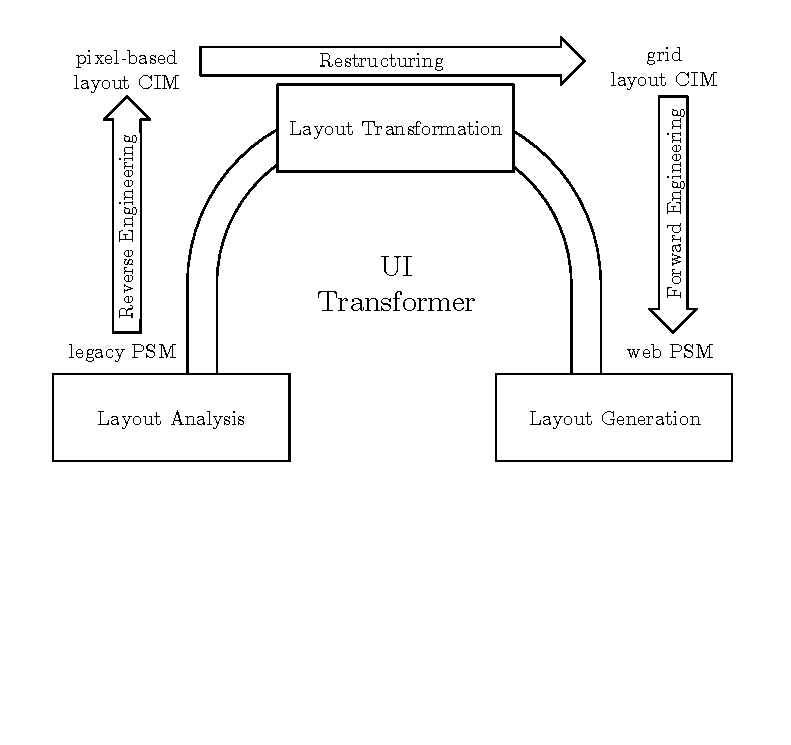
\includegraphics[width=0.7\textwidth]{../figures/awsm-rm-ui-transformation-horseshoe.pdf}
\caption{UI Transformer as model-driven reengineering process}\label{fig:awsm.rm.uitransformer.horseshoe}
}
\end{figure}

%These three stages represent the three parts of an automated, model-driven reengineering horseshoe known from \gls{adm} \autocite{Perez-Castillo2011MARBLE}: reverse engineering as \gls{cim} creation, restructuring as model-to-model transformation between two \glspl{cim}, \gls{Forward Engineering} as model-to-text transformation from \gls{cim} to \gls{psm}.

\vspace{-10pt}
\textbf{Layout Analysis}.
The first stage of UI Transformer extracts the required information according to the \gls{cim}-level formalisms introduced in \cref{sec:ui-formalism} from the input \glspl{artifact}, i.e.~the files \(f \in B_u, B_u \subseteq B\) describing user interface \(u \in U\) of \(\mathfrak{L}\).
In the context of the \gls{mfc} framework used in the scenario, these files are \emph{Resource Files}\footnote{\url{https://docs.microsoft.com/en-us/cpp/ide/resource-files-cpp} Retrieved: 6.12.2019} containing definitions of various application resources.
Using a tool like \emph{Resource Hacker}\footnote{\url{http://www.angusj.com/resourcehacker/} Retrieved: 6.12.2019} they can also be retrieved from executables in \(E\).
Descriptions of user interfaces \(u\) are expressed in \emph{dialog} elements.
\Cref{lst:mfcresource} shows an example of an MFC resource file describing a dialog.
As seen, position and overall viewport of the dialog are stated in the first line, and the three control elements are positioned and sized in pixel units.
UI Transformer parses the resource definitions to extract viewport, controls, types, positions, and sizes.
%Parsing is done based on \emph{regular expressions (RegEx)}.
To determine the \emph{hierarchy} of controls, which occur non-nested in resource files, bounding boxes are tested for complete containment, identifying container and nested container elements, i.e.~the parent controls \(c_p\).
The result of layout analysis is an instance \(l_{legacy}\).

\lstset{
	breaklines=true,
	postbreak=\mbox{$\hookrightarrow$\space}
}
\begin{lstlisting}[language=C++, captionpos=t, caption=Example of a User Interface Description in MFC Resource File (shortened), label=lst:mfcresource]
1 DIALOGEX 0, 0, 289, 90
STYLE DS_MODALFRAME | WS_POPUP | WS_CAPTION | WS_SYSMENU
CAPTION "Appointment Search"
FONT 8, "Tahoma"
{
   ...
   CONTROL "", 6205, COMBOBOX, CBS_DROPDOWNLIST | CBS_SORT | WS_CHILD | WS_VISIBLE | WS_VSCROLL | WS_TABSTOP, 
    7, 71, 152, 30 
   CONTROL "Find", 1, BUTTON, BS_DEFPUSHBUTTON | WS_CHILD | WS_VISIBLE | WS_TABSTOP, 171, 69, 50, 14 
   CONTROL "Cancel", 2, BUTTON, BS_PUSHBUTTON | WS_CHILD | WS_VISIBLE | WS_TABSTOP, 232, 69, 50, 14 
   ...
}
\end{lstlisting}

\vspace{-10pt}
\textbf{Layout Transformation}.
Layout \gls{Transformation} takes \(l_{legacy}\) as input and implements the optimization algorithm in \cref{fig:awsm.rm.uitransformation.process}.
An extract of the implementation is shown in \cref{lst:ui-transformation}, showing the creation of the initial population and subsequent optimization through the evolutionary optimizer.
\Cref{lst:ui-mutation} shows the implementation of mutation of a single layout individual and the crossover of two layouts for the generation of new populations during optimization.
The \gls{Transformation} is computationally complex due to the complexity of the search space \(\mathbb{G}\) with increasing numbers of controls.
Therefore, parallel programming was employed to leverage multi-core processors: \gls{Transformation} is run in parallel for several layout instances \(l_{legacy,i}\) and the calculation of several objective functions \(f_k\) on one \(l_{legacy}\) is also run in parallel.
Our experiments have shown that \emph{processes} are required, since \emph{threads} did not improve performance due to the \emph{Global Interpreter Lock}.
Objective functions \(f_k\) are calculated based \emph{measurements} so that they can reuse measurement results.

The \emph{Levenshtein distance} \autocite{Black2019Levensthein}, used to identify variations in the order of controls \(c \in u\), is a computationally complex measure.
Therefore, a C-based implementation\footnote{\url{https://github.com/ztane/python-Levenshtein/} Retrieved: 6.12.2019} was used for Levenshtein distance calculation.


\begin{lstlisting}[language=Python, captionpos=t, caption=Layout Transformation, label=lst:ui-transformation]
def transform_and_generate_single(self, input_file,
     legacy_layout, silent=True):
  transformer = transformations.SimpleLayoutTransformation()
  initial_grid_layout = transformer.transform(legacy_layout)
  optimizer = EvolutionaryOptimizer(self._target_functions,
    legacy_layout, population_seed=initial_grid_layout)
  optimized_grid_layout = optimizer.optimize(
    self._optimizer_iterations, silent=silent)
  ...      
\end{lstlisting}

\begin{lstlisting}[language=Python, captionpos=t, caption=Mutation and Crossover, label=lst:ui-mutation]

def mutate_individual(self, individual, all_controls=False):
  control_count = len(individual.controls)
  control_index = self.randint(0, control_count - 1)
  control = individual.controls[control_index]
  mutations = [self._mutate_control_xpos,
    self._mutate_control_ypos, self._mutate_control_width,
    self._mutate_control_height] 
  numpy.random.shuffle(mutations)
  ...
  return new_individual
  
  
def crossover_individuals(self, individual1, individual2):
  new_individual = GridLayoutModel(self._input_layout.name,
    self._input_layout.title)   
  controls = self.join(individual1, individual2)
  for (c1, c2) in controls:
    c = copy.deepcopy(c1)
    c.rc.v_start = c2.rc.v_start
    c.rc.v_span = c2.rc.v_span
    new_individual.add_control(c)
  return new_individual
\end{lstlisting}

\pagebreak
\emph{Objective Functions} \(f_k : L_{legacy} \times L_{grid} \mapsto \mathbb{R}_0^+\) compare a \glslink{Legacy System}{legacy} layout instance with a grid layout based on the calculation of measurements on both layouts and a calculation to aggregate the two measurements into a non-negative real number.
The \gls{Transformation} aims at creating grid-based layouts that represent the \glslink{Legacy System}{legacy} layout.
Similarity of layouts is a phenomenon highly related to human perception, not yet very well understood and thus an active field of research (cf.~also \cref{sec:awsm-ci}).
Evolutionary optimization, however, needs a basis for the calculation of fitness.
The objective functions, therefore, represent a set of features that can be automatically calculated from the layout instances without human intervention for fitness calculation.
Five objective functions are implemented: Whitespace Ratio, Control Density, Order of Controls, Edge Alignment, and Area Loss.
Whitespace Ratio \(f_W\) sums the area covered by all visible controls and determines the ratio between this sum and the entire viewport area.
Control Density is a local spatial feature calculated based on Gini coefficient \(f_{D,G}\) and Herfindahl Index \(f_{D,H}\).
Order of Controls \(f_O\) counts changes in order by mapping controls to strings, determining sequences in 8 different orientations (left to right top to bottom, bottom to top right to left, etc.) and calculating the Levenshtein distance of these sequences.
Edge Alignment \(f_A\) identifies aligned vertical and horizontal edges of controls and counts alignment violations in the generated layout.
Area Loss \(f_L\) compares bounding box sizes of controls in both layouts and sums up the differences.

A prototypical alternative implementation of the \gls{Transformation} in C exists, comprising the evolutionary algorithm and the objective function Order of Controls, which is part of experimentation related to performance aspects.
The C-based optimizer integrates with the core python implementation via runtime loading of the library using ctypes\footnote{\url{https://docs.python.org/3/library/ctypes.html} Retrieved: 6.12.2019}.
\Cref{fig:uitransformer.sample} shows an example of a \legacy layout and the resulting transformed version.

\begin{figure}[h!]
\centering

\subfloat[Legacy Layout]{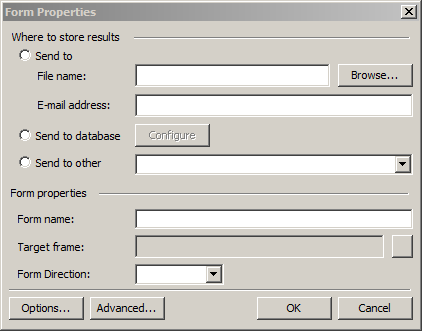
\includegraphics[width=0.36\textwidth]{../figures/uitransformer/3.png}\label{fig:uitransformer.sample-a}}
\qquad
\subfloat[Transformed Layout]{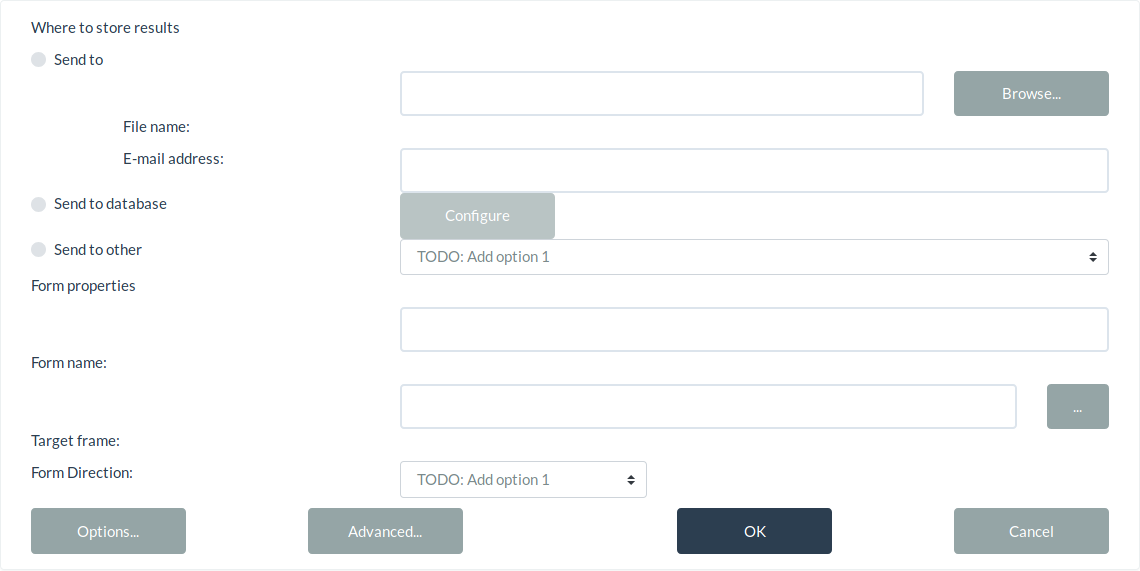
\includegraphics[width=0.56\textwidth]{../figures/uitransformer/3_6.png}\label{uitransformer.sample-b}}

\caption{Layout Transformation Sample}
\label{fig:uitransformer.sample}
\end{figure}

\textbf{Layout Generation}.
The third stage of UI Transformer is a model-to-text generation, taking the \(l_{grid, opt}\) \gls{cim} resulting from the final selection step in \cref{fig:awsm.rm.uitransformation.process} and generating the \gls{psm} of the \gls{wui}, i.e.~an \gls{html} file with corresponding \gls{css} directives, which can be rendered in a \gls{web} browser.
Layouts are generated using bootstrap, as older browsers do not support \gls{css} Grid.
Field research in \cref{sec:research-process}, however, showed that the \gls{isv} customers do not frequently use current operating systems and browsers.
In particular, Internet Explorer 11, does not support \gls{css} Grids.

The \gls{html} output is generated using the Mako\footnote{\url{https://www.makotemplates.org/} Retrieved: 6.12.2019} template engine, allowing to separate design and implementation to facilitate the adaption of the output structure without changes to the generation code.
Generation is based on the hierarchy of controls as represented in the \(c_p\) parent relationships of the \gls{cim} since nested sub-grids can occur.
Controls \(c_1, c_2\) with a common parent element \(c_{1,p}= c_{2,p}\) are grouped by the parent row and then ordered by column.
Iteration over the hierarchy starts with root-level elements (having \(c_p = 0\)) based on a pointer indicating the current position within the grid for cell offset calculation.
The text is generated using the template engine, line by line and cell by cell and recursion for each container element, creating a sub-grid.
Representation of controls is based on a mapping from \gls{mfc} controls to \gls{html} elements.
A placeholder is generated for controls without \gls{html} equivalent (e.g.~scrollbar), which can be implemented as custom element using WebComponents.
\Cref{lst:ui-generation} shows the implementation of the layout generation, filling the cells and rows in a bootstrap grid layout.

%\pagebreak
\begin{lstlisting}[language=Python, captionpos=t, caption=Layout Generation, label=lst:ui-generation]
def generate_grid(self, layout, parent_id=None):
 filtered_controls = layout.controls_by_parent(parent_id)
 o_controls = SortedDict()
 for c in filtered_controls:
  row_key = c.rc.v_start
  if row_key not in o_controls:
   controls_in_cell = SortedList(
    [c], key=lambda x: x.rc.h_span * x.rc.v_span
   )
   cells_in_row = SortedDict()
   cells_in_row[c.rc.h_start] = controls_in_cell
   o_controls[row_key] = cells_in_row
  else:
   column_key = c.rc.h_start
   if column_key not in o_controls[row_key]:
    controls_in_cell = SortedList(
     [c], key=lambda x: x.rc.h_span * x.rc.v_span
    )
    o_controls[row_key][column_key] = controls_in_cell
   else:
    o_controls[row_key][column_key].add(c)
 self._current_position = Rectangle(0, 0, None, None)
 r_code = []
 for row in o_controls.keys():
  self._current_position.h_start = 0
  self._current_position.v_start = row
  assert len(o_controls[row]) > 0 
  r_code.append(self.generate_grid_row(
   layout, o_controls[row]
  ))
 layout_text = '\n'.join(r_code) if len(r_code) > 0 else ''
 page_template = templ_lookup.get_template('/grid.html')
 output_text = page_template.render(grid_rows=layout_text)
 return output_text
\end{lstlisting}

\vspace{-15pt}
\hypertarget{sec:rm.evaluation}{%
\section{Evaluation}\label{sec:rm.evaluation}}
\vspace{15pt}

This section evaluates AWSM:RM regarding different aspects.
\Cref{sec:rm.evaluation.req} evaluates AWSM:RM against the requirements in \cref{sec:rm.requirements}.
Three additional experimental evaluations further address the effectiveness, efficiency, and expertise in \cref{sec:rewamp.experiment}, \cref{sec:rwmpa.experiment}, and \cref{sec:uitransformer.experiment}.
\Cref{sec:rm.evaluation.objective} revisits research objective \cref{ro:2} in the light of the evaluation results.

%\vspace{-10pt}
\hypertarget{sec:rm.evaluation.req}{%
\subsection{Assessment of Requirements}\label{sec:rm.evaluation.req}}
\vspace{10pt}

This section reports on satisfaction of the requirements for AWSM:RM.

\textbf{Effectiveness}.
The effectiveness of AWSM:RM is achieved through specification of a \gls{Web Migration} prototyping technique that creates concrete, tangible \glspl{web migration prototype} which can be used to demonstrate desirability and feasibility of \gls{Web Migration}.
A detailed evaluation of results quality is presented in the following evaluation experiments.

\vspace{-10pt}
\textbf{Efficiency}.
The efficiency of AWSM:RM is achieved through reuse of business logic via a semi-automatic WebAssembly-based compilation process and runtime environment and an automatic model-driven \gls{Transformation} process converting \glslink{Legacy System}{legacy} pixel-based user interfaces into grid-based \gls{web} user interfaces.
A detailed evaluation showing the results achievable with limited and no manual interventions is presented in the following evaluation experiments, reporting on time measurements.

\vspace{-10pt}
\textbf{Expertise}.
The expertise requirement is addressed in AWSM:RM in two ways: the business logic reuse process focuses on the existing expertise of the Prototyping Engineer in the \glslink{Legacy System}{legacy} platform and lowers the required \gls{Web Engineering} and migration expertise requirements by providing a semi-automatic process with a guidance system including explanations and support tools.
The \gls{Web Engineering} expertise generally required for the creation of \glslink{web}{Web}-based user interfaces is avoided through a fully automatic process without manual interventions.
The following evaluation experiments demonstrate the applicability of AWSM:RM with test subjects with limited \gls{Web Engineering} and no \gls{Web Migration} expertise.
AWSM:RM meets the expertise requirement as it is a feasible method based on available expertise with limited \gls{Web Engineering} and no \gls{Web Migration} expertise.

\vspace{-10pt}
\textbf{Reuse}.
The AWSM:RM method focuses on reuse as key enabler for the rapidness of \web migration prototyping.
It reuses both \glslink{Legacy System}{legacy} business logic through the WebAssembly-based \gls{rewamp} process and \glslink{Legacy System}{legacy} user interfaces through the automatic creation of \glspl{wui} based on an automated model-driven \gls{Transformation} abstracting from the \glslink{Legacy System}{legacy} \gls{ui} \gls{psm} to a pixel-based layout \gls{cim}, transforming it into a grid-based layout \gls{cim} and generating the \gls{wui} \gls{psm}.
AWSM:RM fulfills the reuse requirement as it is based on reuse on both layers of horizontal prototypes: the user interface and the business logic.

\vspace{-10pt}
\textbf{Plausibility}.
The \glspl{web migration prototype} resulting from AWSM:RM are \glspl{Web Application} using the standard \gls{web} technology stack of \gls{html}, \gls{css}, and JavaScript in addition to the new WebAssembly standard.
Unlike wrapper approaches, they run entirely independent of the \gls{Legacy System}, and they run in any major \gls{web} browser without additional requirements such as extensions, plugins, etc.
The architecture of the \glspl{web migration prototype} represents the major architectural changes of \gls{Web Migration}: client/server communication, URL-based navigation, encapsulation of the persistence layer behind a \glslink{rest}{RESTful} \gls{api}.
AWSM:RM fulfills the plausibility requirements as its prototypes are demonstrative \glspl{Web Application} representative of all major \gls{Web Application} characteristics.

\vspace{-15pt}
\hypertarget{sec:rewamp.experiment}{%
\subsection{Experimental Evaluation of ReWaMP}\label{sec:rewamp.experiment}}
\vspace{5pt}

Experimental evaluation of \gls{rewamp} focuses on the aspects of time and effort for \gls{rewamp}, on required expertise of the Prototyping Engineer, on a detailed understanding of the most prolonged/most difficult tasks in \gls{rewamp} and on possible results from the application of \gls{rewamp}.

\textbf{Setup}.
The basis for experimentation is the medical appointment scheduling scenario application, as characterized in \cref{sec:scenario-code}.
The scenario codebase \(B\) comprises 3373 \gls{loc}, of which the \emph{test dataset} \(B_T \subset B\) contains the 3 main views \(B_T = \{u_{cal}, u_{appointments}, u_{new}\}\) shown in \cref{fig:rewamp-myCal}.
The test dataset \(B_T\) comprises 937 \gls{sloc} defining 35 types, 237 methods, and using 177 third-party elements.
Additionally, an executable \(e \in E\) of the \glslink{Legacy System}{legacy} application was available.
The evaluation platform was a Windows 10 Education N x64 running on an Intel i7 930 CPU (2,8GHz), 14 GB RAM.

The experiment was conducted through observed test runs of the \gls{rewamp} process with test subjects.
The \emph{test subjects} impersonated the role of Prototyping Engineer and were observed during execution by a \emph{researcher}.
\Cref{tbl:rewamp.guidelines} shows the guidelines for interaction of the researcher and the test subject.
The questionnaire shown in \cref{sec:rewamp-questionaire} implemented as Google Form was set up to capture test subject data and subjective perceptions of the \gls{rewamp} process and \gls{wasmt} tool support.
\begin{figure}[h!]
    \centering
    \subfloat[Calendar Dialog $u_{cal}$]{
        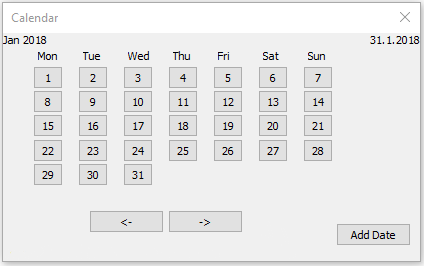
\includegraphics[width=0.49\textwidth]{../figures/screenshots/MyCal-Cal01.PNG}
        \label{fig:rewamp-myCal-a}}
    \subfloat[Appointments View $u_{appointments}$]{
        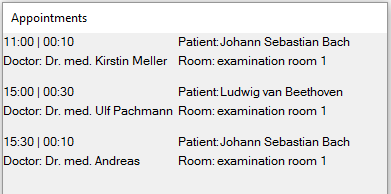
\includegraphics[width=0.49\textwidth]{../figures/screenshots/MyCal-appoints.PNG}
        \label{fig:rewamp-myCal-b}}
    \qquad
    \subfloat[New Appointment Dialog $u_{new}$]{
        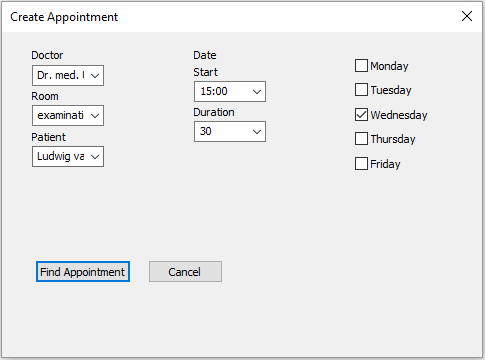
\includegraphics[width=0.49\textwidth]{../figures/screenshots/MyCal-Date.PNG}
        \label{fig:rewamp-myCal-c}}
    \caption{Test Dataset $B_T$ Views}
    \label{fig:rewamp-myCal}
\end{figure}

\textbf{Procedure}.
Each test subject attended a brief introduction to the scenario, its context visualized as \cref{fig:awsm.rm.overview}, and the \gls{rewamp} process visualized as \cref{fig:awsm.rm.rewamp.process}.
The executable \(e \in E\) of the scenario application was available for the test subjects to explore the functionality.
The researcher supervised the test run by setting up the required tools, backing up intermediate results, and providing the same environment state for each step for each test subject, strictly following the guidelines.
The test subjects followed the sequence of steps of \gls{rewamp} and performed the manual tasks, extracting BBL files from \(B\), configuring \gls{wasmt}, and applying expert interventions (expert changes and expert files).
Clion\footnote{\url{https://www.jetbrains.com/clion/} Retrieved: 6.12.2019} was used by the test subjects to navigate the codebase and perform expert interventions; Windows Explorer was used for task 1: one window showing the codebase \(B_T\) and one window the working directory of \gls{wasmt}.
To reduce the time required for one evaluation run, tasks 2, 4 and 5 were conducted only for the two more complex views \(u_{cal}\) and \(u_{new}\).
At the end of each test run, the test subject had 5 minutes to familiarise with the migration prototype, before answering the questionnaire.

In addition to the subjective perceptions captured in the questionnaire, objective observations were made through measurements.
As \gls{Rapid Prototyping} implies quick and easy creation of prototypes, time and effort were measured during the experiment for each task.

\emph{Time} \(t = t_M + t_T\) has two main components, \(t_M\) the time required by the Prototyping Engineer to perform the manual tasks (1,2,4,5) in \cref{fig:awsm.rm.rewamp.process}, and \(t_T\) the time required by \gls{wasmt} to analyze and transform the \glslink{Legacy System}{legacy} code.
\(t_M\) was measured by stopwatch, \(t_T\) was measured programmatically.
Time measurement started at the start of manual tasks after preparation of the tools, was interrupted if \gls{wasmt} started or resumed processing, and ended by finishing the last expert interventions.
\(t_T\) is a system environment-dependent measure: on the evaluation platform described above, 87 other processes were active during measurement, and an average load of 13,8\% was determined.

\emph{Effort} evaluates the amount and extent of changes to the existing \glslink{Legacy System}{legacy} code required by \gls{rewamp}.
Effort can be measured in terms of \emph{code churn}, i.e. the lines of code added/changed/deleted, which has been shown to have a strong linear correlation with effort \autocite{Sjoberg2013}.
Thus, \(e_T\) represents the code churn (\gls{sloc}) by \gls{wasmt} and
\(e_M\) the code churn by the Prototyping Engineer.
\(e_M\) was measured through observation of the test subject and \(e_T\) by comparison of inputs and results of one continuous task set completion.
All efforts were measured per task and per category (create, update, delete).

\textbf{Experimental results and descriptive statistics}.
The experiment was conducted with 6 test subjects (5 male, 1 female), with an age range of 23 -- 35 (mean 26), 2-10 years of programming experience (mean 6.33) and \gls{Web Engineering} expertise (mean 2.83 on Likert scale 1-5).
\Cref{tbl:rewamp-timeresults} provides an overview of the time results.
The test runs' overall time was between 01:14:27h and 02:06:36h, (mean 01:38:27), which includes processing views as described above.
Averaged for one complete process instance of one view, time \(t\) was between 00:38:07h and 01:05:13h (\(\overline t\) = 00:50:24h), of which an almost constant (\(\sigma\) = 2s) time of \(\overline{t_T}\) = 00:00:47h was required by \gls{wasmt}.
The average time for manual tasks was \(\overline{t_M}=\) 00:49:36h (\(\sigma\) = 00:10:06h).
Considering time distribution on the tasks shown in \cref{fig:awsm.rm.rewamp.timetask}, task 4 (expert changes) took the longest (\(\approx\) 61\% of \(t\)), followed by task 1 (\(\approx\) 23\% of \(t\)).
For task 4 and 5, times for \(u_{cal}\) (\(t4.1, t5.1,\)) and \(u_{new}\) (\(t4.2, t5.2\)) are shown separately.
While task 4 times are close, for task 5 (expert file) \(u_{cal}\) was faster than \(u_{new}\).


\begin{xltabular}{\linewidth}[hbt]{@{}llllllll@{}}
\caption{\label{tbl:rewamp-timeresults}ReWaMP Time Measurement Statistics}\tabularnewline
\toprule
\begin{minipage}[b]{0.07\columnwidth}\raggedright
\(\bm{\overline{t_M}}\)\strut
\end{minipage} & \begin{minipage}[b]{0.07\columnwidth}\raggedright
\(\bm{\overline{t_T}}\)\strut
\end{minipage} & \begin{minipage}[b]{0.07\columnwidth}\raggedright
\(\bm{\sigma(t_M)}\)\strut
\end{minipage} & \begin{minipage}[b]{0.07\columnwidth}\raggedright
\(\bm{\sigma(t_T)}\)\strut
\end{minipage} & \begin{minipage}[b]{0.07\columnwidth}\raggedright
\(\bm{\overline{t1}}\)\strut
\end{minipage} & \begin{minipage}[b]{0.07\columnwidth}\raggedright
\(\bm{\overline{t2}}\)\strut
\end{minipage} & \begin{minipage}[b]{0.07\columnwidth}\raggedright
\(\bm{\overline{t4}}\)\strut
\end{minipage} & \begin{minipage}[b]{0.08\columnwidth}\raggedright
\(\bm{\overline{t5}}\)\strut
\end{minipage}\tabularnewline
\midrule
\endfirsthead
\toprule
\begin{minipage}[b]{0.07\columnwidth}\raggedright
\(\bm{\overline{t_M}}\)\strut
\end{minipage} & \begin{minipage}[b]{0.07\columnwidth}\raggedright
\(\bm{\overline{t_T}}\)\strut
\end{minipage} & \begin{minipage}[b]{0.07\columnwidth}\raggedright
\(\bm{\sigma(t_M)}\)\strut
\end{minipage} & \begin{minipage}[b]{0.07\columnwidth}\raggedright
\(\bm{\sigma(t_T)}\)\strut
\end{minipage} & \begin{minipage}[b]{0.07\columnwidth}\raggedright
\(\bm{\overline{t1}}\)\strut
\end{minipage} & \begin{minipage}[b]{0.07\columnwidth}\raggedright
\(\bm{\overline{t2}}\)\strut
\end{minipage} & \begin{minipage}[b]{0.07\columnwidth}\raggedright
\(\bm{\overline{t4}}\)\strut
\end{minipage} & \begin{minipage}[b]{0.08\columnwidth}\raggedright
\(\bm{\overline{t5}}\)\strut
\end{minipage}\tabularnewline
\midrule
\endhead
\begin{minipage}[t]{0.07\columnwidth}\raggedright
49:36\strut
\end{minipage} & \begin{minipage}[t]{0.07\columnwidth}\raggedright
00:47\strut
\end{minipage} & \begin{minipage}[t]{0.07\columnwidth}\raggedright
10:06\strut
\end{minipage} & \begin{minipage}[t]{0.07\columnwidth}\raggedright
2s\strut
\end{minipage} & \begin{minipage}[t]{0.07\columnwidth}\raggedright
11:22\strut
\end{minipage} & \begin{minipage}[t]{0.07\columnwidth}\raggedright
02:20\strut
\end{minipage} & \begin{minipage}[t]{0.07\columnwidth}\raggedright
30:49\strut
\end{minipage} & \begin{minipage}[t]{0.08\columnwidth}\raggedright
05:06\strut
\end{minipage}\tabularnewline
\bottomrule
\end{xltabular}

\begin{figure}[hbt]
\hypertarget{fig:awsm.rm.rewamp.timetask}{%
\centering
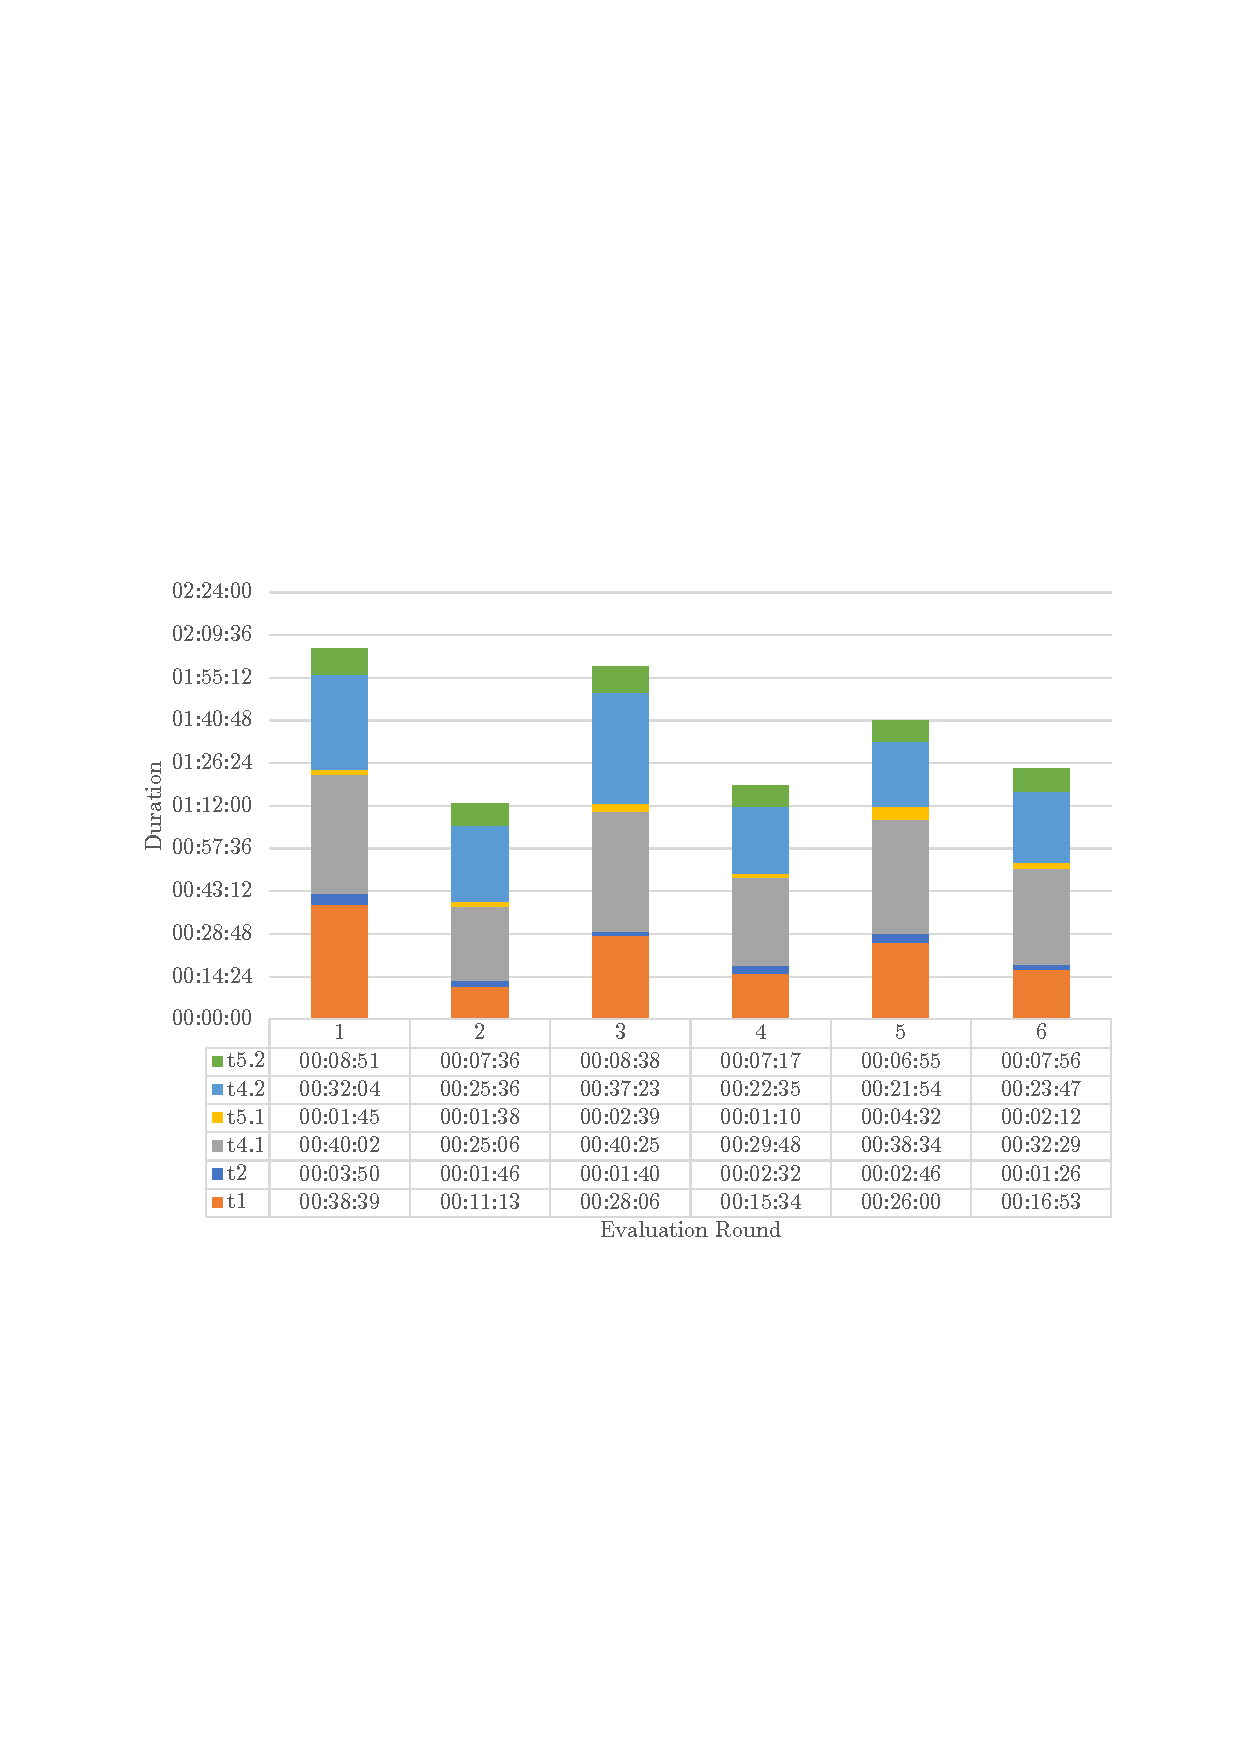
\includegraphics[width=0.99\textwidth]{../figures/rewamp/time-task.pdf}
\caption{Time distributions per task and test run}\label{fig:awsm.rm.rewamp.timetask}
}
\end{figure}

\vspace{-15pt}
\Cref{tbl:rewamp-effortresults} provides an overview of the effort results, averaged over the test subjects per on view.
\Cref{fig:efforts} shows the effort distributions.
\gls{wasmt} performs almost \(3/4\) of all required changes (\cref{fig:efforts-a}).
The manual effort \(e_M\) (\cref{fig:efforts-c}) distribution shows that the Prototyping Engineer mainly performs delete operations, whereas \(2/3\) of the automatic changes \(e_T\) from \gls{wasmt} (\cref{fig:efforts-d}) add code.

\begin{xltabular}{\linewidth}[b!]{@{}llllllllll@{}}
\caption[Effort Measurement Statistics]{\label{tbl:rewamp-effortresults}Effort Measurement Statistics, in SLOC}\tabularnewline
\toprule
\begin{minipage}[b]{0.05\columnwidth}\raggedright
\(\bm{\overline{e_M}}\)\strut
\end{minipage} & \begin{minipage}[b]{0.05\columnwidth}\raggedright
\(\bm{\overline{e_T}}\)\strut
\end{minipage} & \begin{minipage}[b]{0.09\columnwidth}\raggedright
\(\bm{\sigma(e_M)}\)\strut
\end{minipage} & \begin{minipage}[b]{0.09\columnwidth}\raggedright
\(\bm{\sigma(e_T)}\)\strut
\end{minipage} & \begin{minipage}[b]{0.05\columnwidth}\raggedright
\(\bm{\overline{e_M^C}}\)\strut
\end{minipage} & \begin{minipage}[b]{0.05\columnwidth}\raggedright
\(\bm{\overline{e_M^U}}\)\strut
\end{minipage} & \begin{minipage}[b]{0.05\columnwidth}\raggedright
\(\bm{\overline{e_M^D}}\)\strut
\end{minipage} & \begin{minipage}[b]{0.05\columnwidth}\raggedright
\(\bm{\overline{e_T^C}}\)\strut
\end{minipage} & \begin{minipage}[b]{0.05\columnwidth}\raggedright
\(\bm{\overline{e_T^U}}\)\strut
\end{minipage} & \begin{minipage}[b]{0.05\columnwidth}\raggedright
\(\bm{\overline{e_T^D}}\)\strut
\end{minipage}\tabularnewline
\midrule
\endfirsthead
\toprule
\begin{minipage}[b]{0.05\columnwidth}\raggedright
\(\bm{\overline{e_M}}\)\strut
\end{minipage} & \begin{minipage}[b]{0.05\columnwidth}\raggedright
\(\bm{\overline{e_T}}\)\strut
\end{minipage} & \begin{minipage}[b]{0.09\columnwidth}\raggedright
\(\bm{\sigma(e_M)}\)\strut
\end{minipage} & \begin{minipage}[b]{0.09\columnwidth}\raggedright
\(\bm{\sigma(e_T)}\)\strut
\end{minipage} & \begin{minipage}[b]{0.05\columnwidth}\raggedright
\(\bm{\overline{e_M^C}}\)\strut
\end{minipage} & \begin{minipage}[b]{0.05\columnwidth}\raggedright
\(\bm{\overline{e_M^U}}\)\strut
\end{minipage} & \begin{minipage}[b]{0.05\columnwidth}\raggedright
\(\bm{\overline{e_M^D}}\)\strut
\end{minipage} & \begin{minipage}[b]{0.05\columnwidth}\raggedright
\(\bm{\overline{e_T^C}}\)\strut
\end{minipage} & \begin{minipage}[b]{0.05\columnwidth}\raggedright
\(\bm{\overline{e_T^U}}\)\strut
\end{minipage} & \begin{minipage}[b]{0.05\columnwidth}\raggedright
\(\bm{\overline{e_T^D}}\)\strut
\end{minipage}\tabularnewline
\midrule
\endhead
\begin{minipage}[t]{0.05\columnwidth}\raggedright
121\strut
\end{minipage} & \begin{minipage}[t]{0.05\columnwidth}\raggedright
338\strut
\end{minipage} & \begin{minipage}[t]{0.09\columnwidth}\raggedright
4.5\strut
\end{minipage} & \begin{minipage}[t]{0.09\columnwidth}\raggedright
4.5\strut
\end{minipage} & \begin{minipage}[t]{0.05\columnwidth}\raggedright
34\strut
\end{minipage} & \begin{minipage}[t]{0.05\columnwidth}\raggedright
22\strut
\end{minipage} & \begin{minipage}[t]{0.05\columnwidth}\raggedright
65\strut
\end{minipage} & \begin{minipage}[t]{0.05\columnwidth}\raggedright
224\strut
\end{minipage} & \begin{minipage}[t]{0.05\columnwidth}\raggedright
62\strut
\end{minipage} & \begin{minipage}[t]{0.05\columnwidth}\raggedright
54\strut
\end{minipage}\tabularnewline
\bottomrule
\end{xltabular}

%todo{TODO:UPDATE NUMBERS FROM TABLE}

\begin{figure}
\centering

\subfloat[Average \(e\) Distribution]{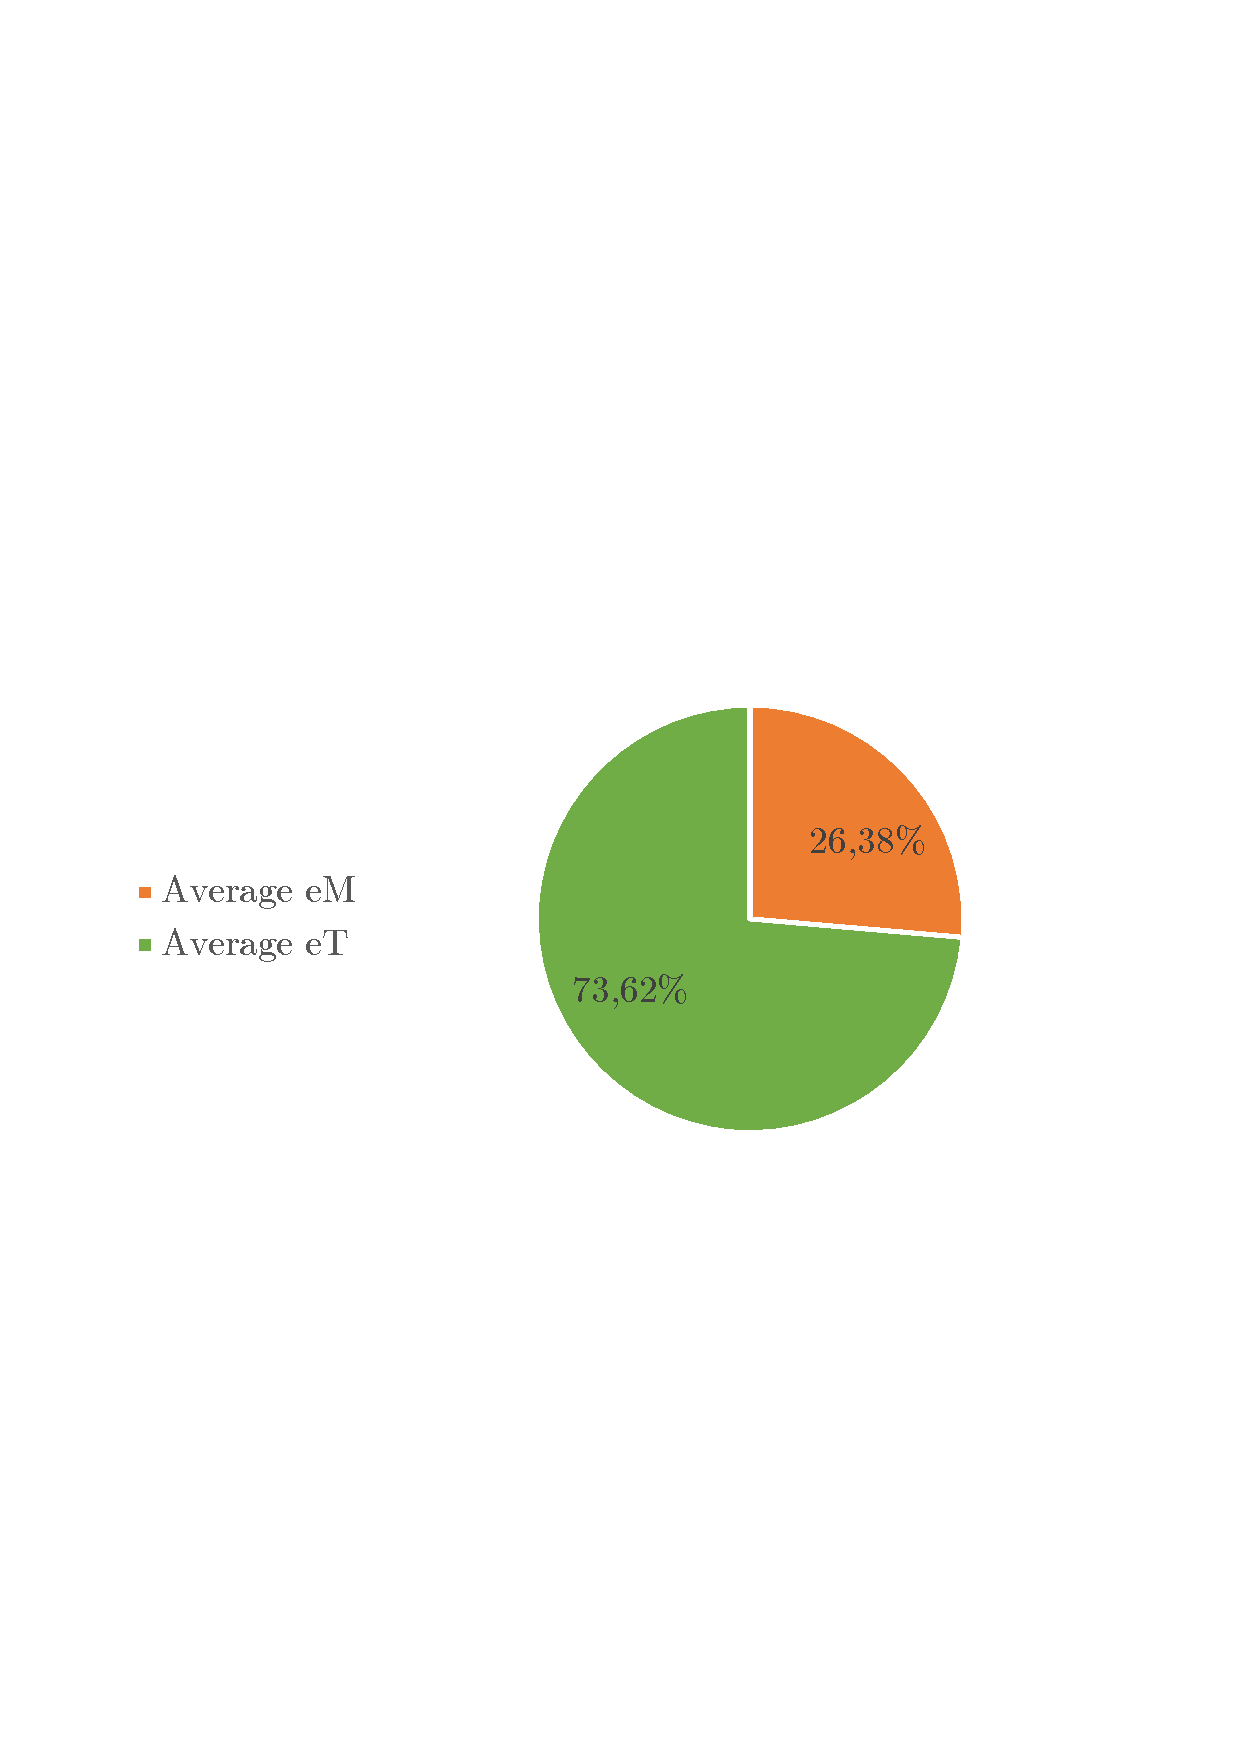
\includegraphics[width=0.42\textwidth]{../figures/rewamp/efforts-a.pdf}\label{fig:efforts-a}}
\subfloat[Average \(e_M\) Distribution]{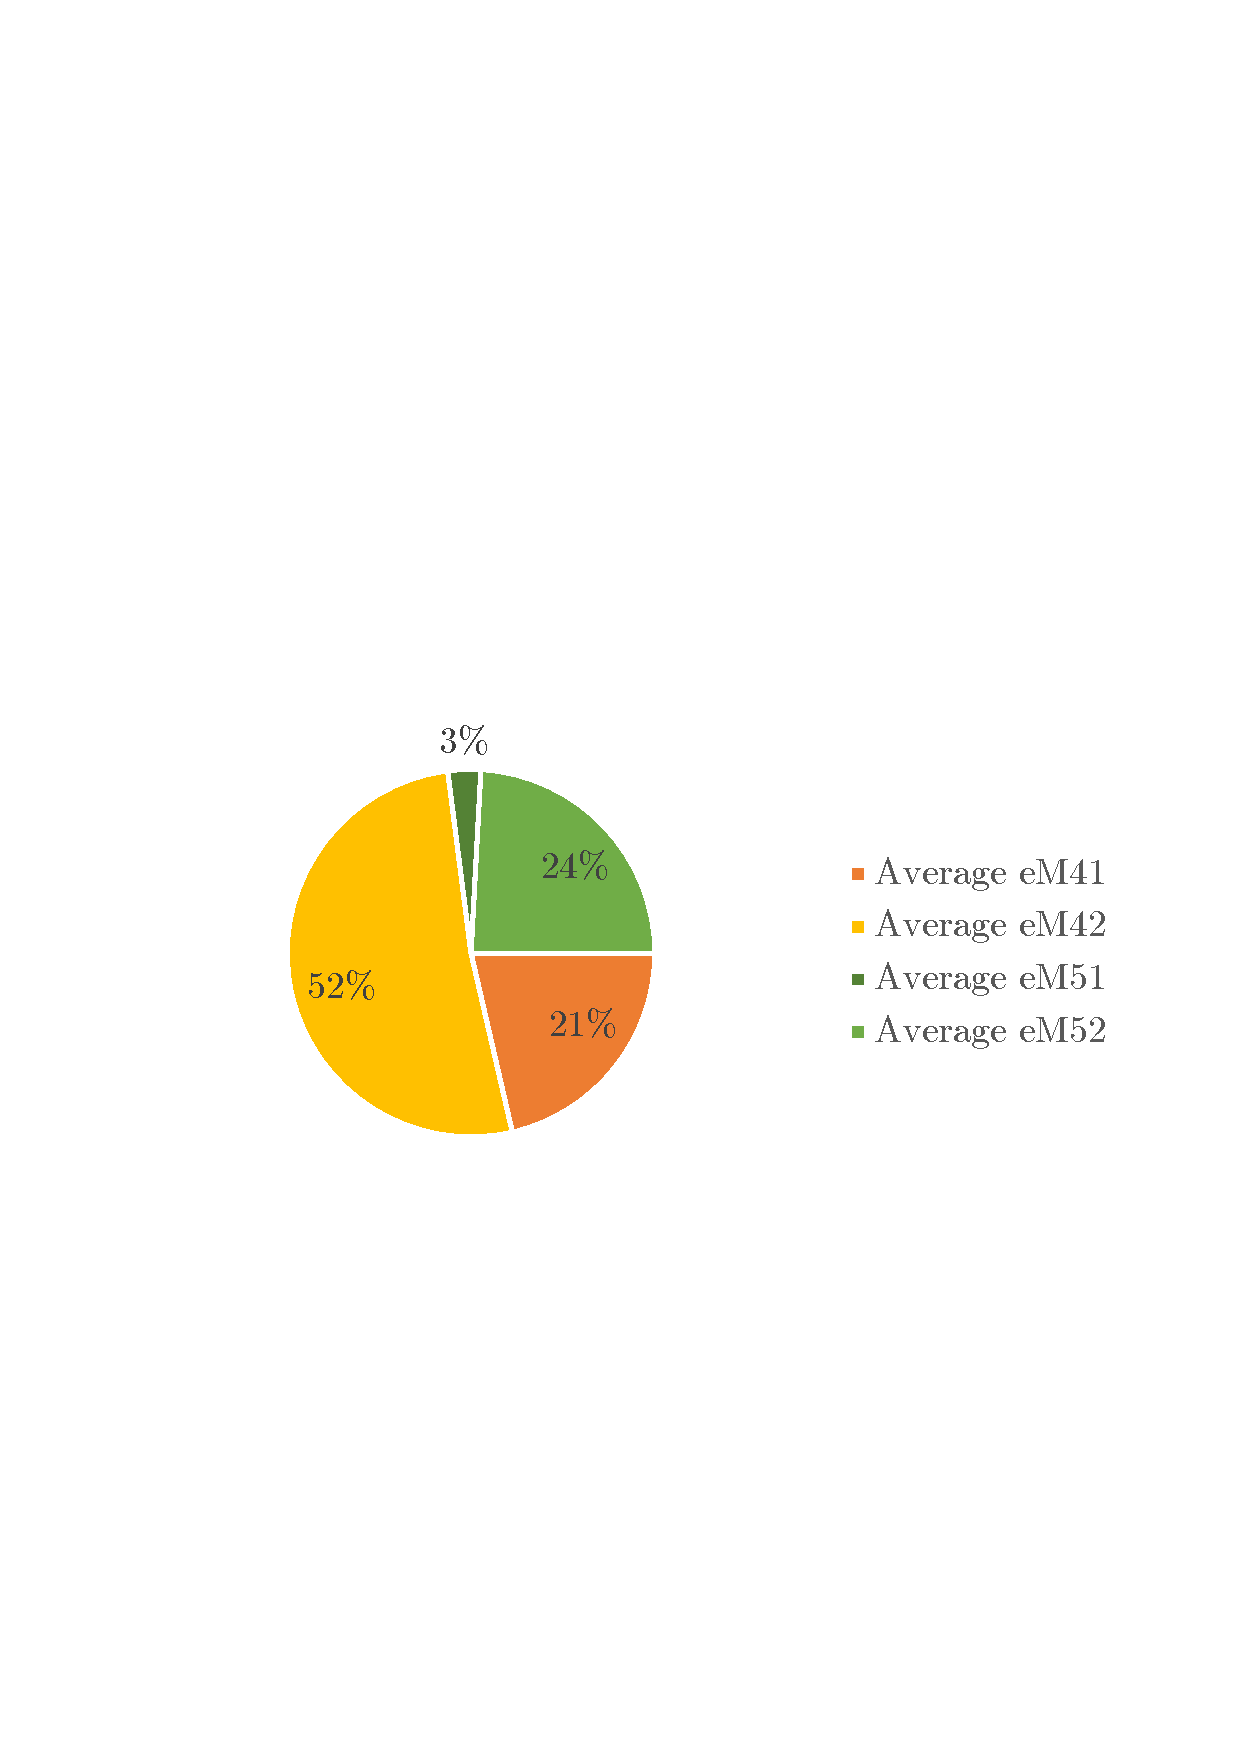
\includegraphics[width=0.42\textwidth]{../figures/rewamp/efforts-b.pdf}\label{fig:efforts-b}}

\subfloat[Average \(e_M\) Distribution by CUD]{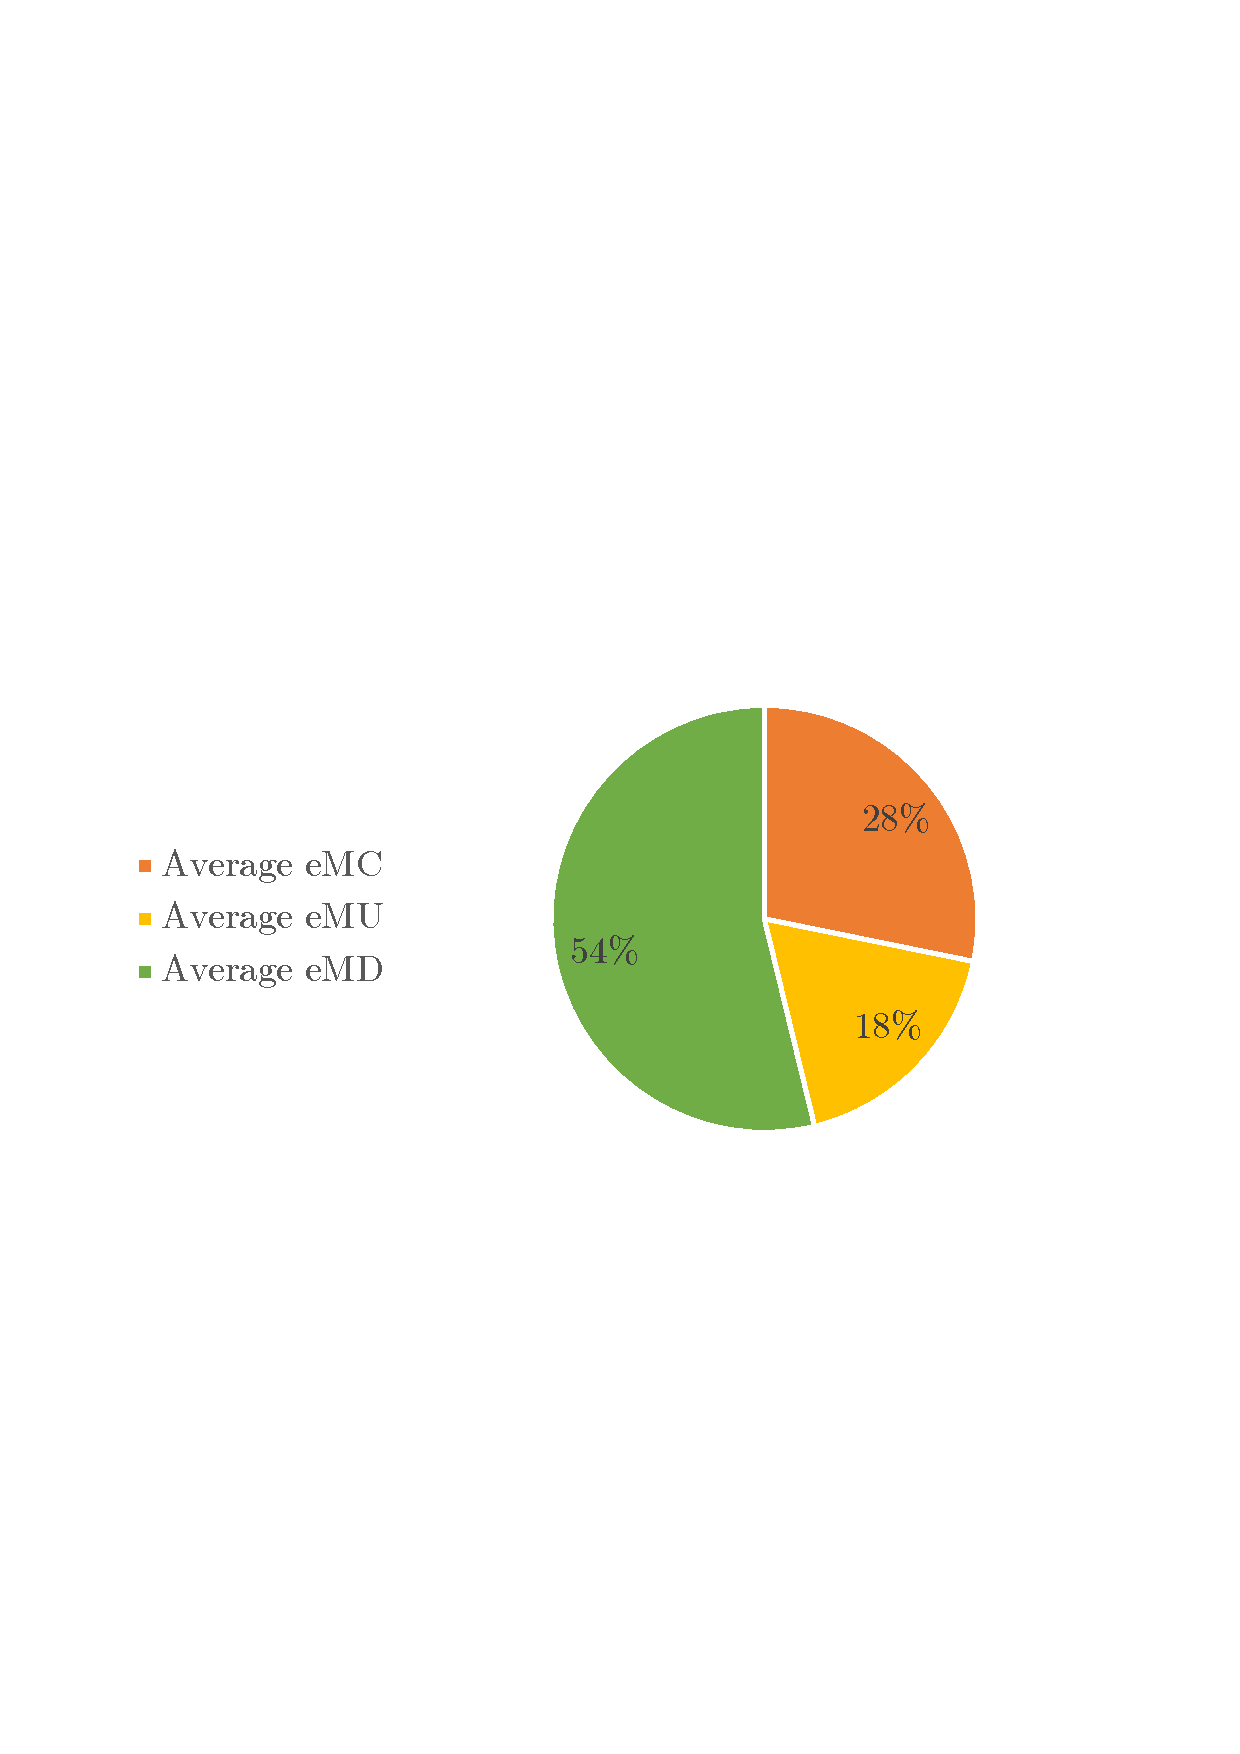
\includegraphics[width=0.42\textwidth]{../figures/rewamp/efforts-c.pdf}\label{fig:efforts-c}}
\subfloat[Average \(e_T\) Distribution by CUD]{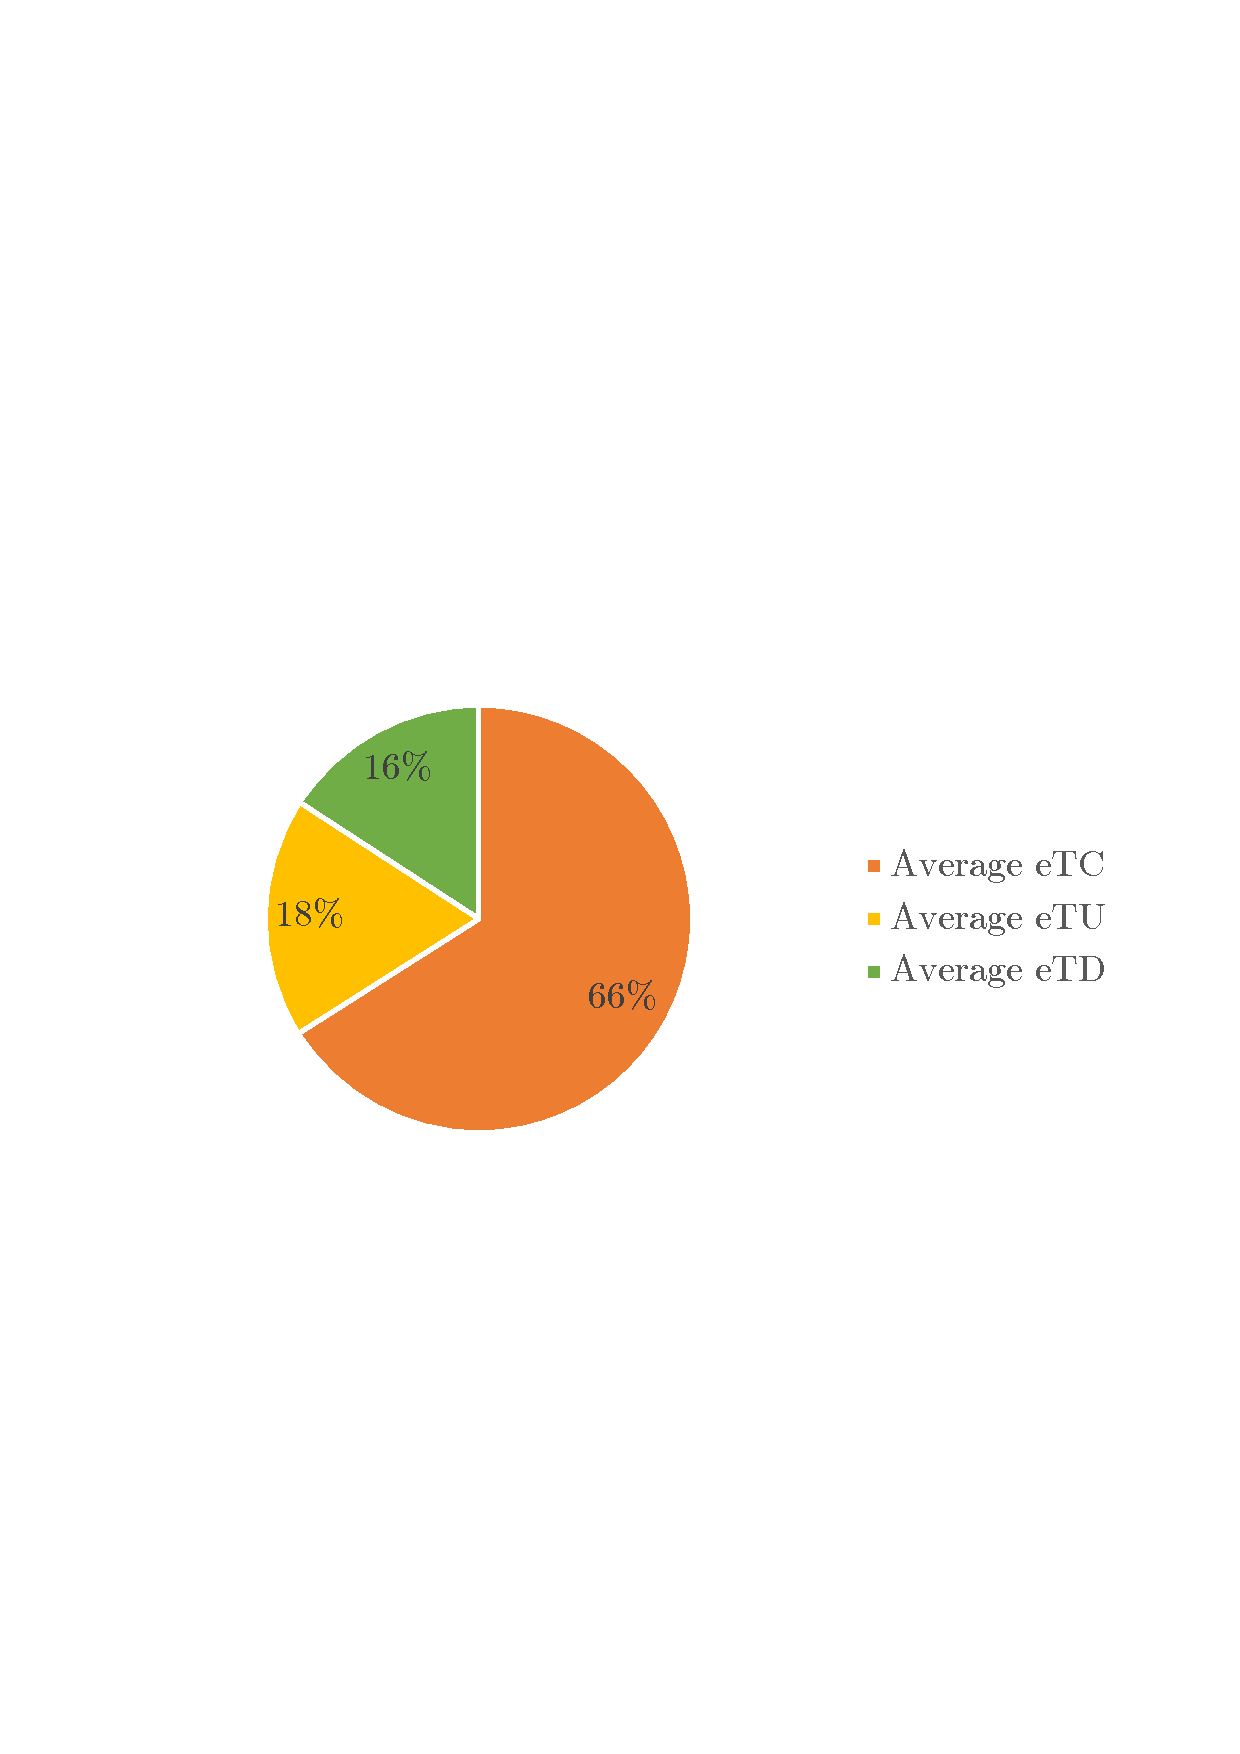
\includegraphics[width=0.42\textwidth]{../figures/rewamp/efforts-d.pdf}\label{fig:efforts-d}}

\caption{Effort Distributions}
\label{fig:efforts}
\end{figure}

%\vspace{-55pt}
\Cref{fig:rewamp.boxplot} shows the questionnaire results.
As can be seen, understanding of the \gls{rewamp} process was rated very differently across the test subjects, but overall not easy (median 2).
\pagebreak
The manual work required is considerable, rated medium (median 3), but test subjects agreed that \gls{wasmt} took over a large share of work and that without \gls{wasmt} the work would have been significantly more extensive (both median 4).
The process was considered medium short (median 3) and subjects agreed that without \gls{wasmt} it would have taken significantly longer (median 4.5).

\begin{figure}
\hypertarget{fig:rewamp.boxplot}{%
\centering
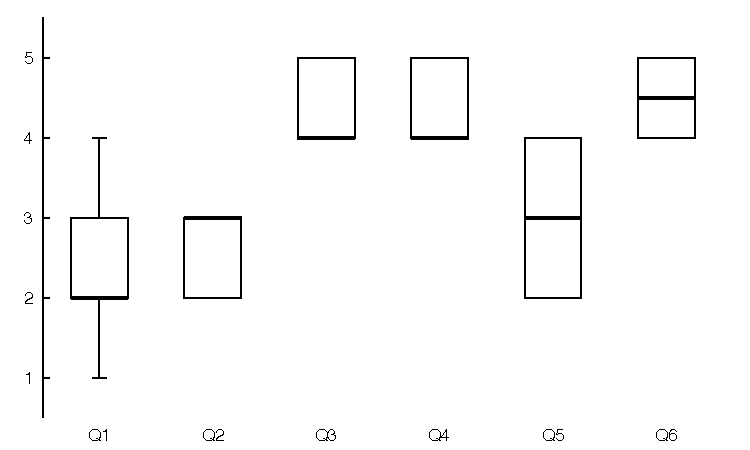
\includegraphics[width=0.7\textwidth]{../figures/boxplots/rewamp-boxplot.pdf}
\caption[ReWaMP Questionnaire Results]{ReWaMP Questionnaire Results, 5-level Likert scale, Q1 ReWaMP easy to understand, Q2 manual work for ReWaMP, Q3 WASM-T did much work, Q4 without WASM-T more work, Q5 process was short, Q6 without WASM-T more time}\label{fig:rewamp.boxplot}
}
\end{figure}

A live example of a \gls{rewamp} prototype created during evaluation and its \gls{wasm} source are available online\footnote{\url{https://vsr.informatik.tu-chemnitz.de/demos/ReWaMP} Retrieved: 6.12.2019}, a screenshot of this prototype is shown in \cref{fig:awsm.rm.prototype-screenshot}.

\textbf{Analysis}. The measured times show a high variation in the time for manual tasks (\(\sigma\) about 10min, i.e.~about 20\% of \(t_M\)).
These variations are highly dependent (Pearson's \(\rho=-0.823\), \(p=0.0442\), highly significant at \(\alpha = 0.05\)) on the programming expertise of the Prototyping Engineer: the more experienced the test subject, the lower \(t_M\).
Considering that the \gls{rewamp} process was new to the test subjects, the measured times are rather short with the first view, \(u_{cal}\) finished in less than 45 minutes.
As expected, the expert interventions took the largest share of time.
The relatively long time for task 1 was not expected and may be the result of two factors: low decomposability/readability of the \glslink{Legacy System}{legacy} code and unfamiliarity with code base.

While the latter problem would not be faced to the same extent by Prototyping Engineers from the \gls{isv}, the former represents a relevant characteristic in \gls{Web Migration}.
The apparent increase in time for task 5 (expert file) between \(u_{cal}\) and \(u_{new}\) represents a difference in the complexity of these views: while the expert file for \(u_{cal}\) must contain only two empty functions, the expert file for \(u_{new}\) is considerably more complex as it requires mock classes for room, doctor, patient, etc.

Effort measurements show little variation, neither for manual nor \gls{wasmt} tasks (\(\sigma = 4.5\) for both), because for the same views, very similar code changes were required.
This is also an indicator of a relatively low complexity of the changes since more complex code would show more variety, depending on the test subjects' expertise.
The overall manual effort of 121 \gls{sloc} per view is relatively small, in particular, compared to the 338 \gls{sloc} of changes by \gls{wasmt}.
Analysis of the effort distribution in the create/update/delete categories shows that the Prototyping Engineer performs mainly simple delete operations.
In contrast, \gls{wasmt} mainly adds code.
Similar to time analysis, the higher complexity of \(u_{new}\) shows in the difference of manual efforts for task 5: \(u_{cal}\) has \(\overline{e_M^{5,1}}=7\) \gls{sloc}, compared to \(u_{new}\) with \(\overline{e_M^{5,2}}=59\) \gls{sloc}, due to the more complex expert file required.
There is no significant correlation between measured times and measured efforts.
The subjective perceptions of test subjects ranked manual work effort medium, but are in agreement with the objective effort distribution that \gls{wasmt} took over a large share of work, and without the tool support, their work would have been more extensive.

\textbf{Threats to Validity}.
\emph{Construct validity} of this experiment is threatened by possible variations in the execution of the test runs.
This was addressed through the provision of the same, well-defined state for all test subjects.
Identical execution of the test runs was achieved due to the underlying formalized \gls{rewamp} process.
The time and effort measurements of the experiment address the two main characteristics of \gls{Rapid Prototyping}.

\emph{Internal validity} of this experiment is threatened through potential subjective biases.
This was addressed through the establishment of guidelines that strictly governed interactions between test subjects and the researcher.
While some test subjects might have been biased towards providing slightly positive responses to the survey, the design of the evaluation experiment combining the subjective perceptions with objective time and effort measurements still provides a reasonable basis for an analysis of overall complexity, comparison of tasks and effort distribution between manual tasks and tasks automated in the toolchain.

\emph{External validity} of the experiment is threatened through limitations in the generalizability of results.
The main factor is the test subjects, that are from a similar age and experience range.
However, the low \gls{Web Engineering} expertise in comparison to general programming expertise represents an essential characteristic of the \gls{migrationengineer} stakeholder group.
To increase generalizability, a large-scale study with test subjects from different \glspl{isv} would be required.
While these studies are feasible in the context of funded research projects -- a single test run requires between 1.25 to more than 2 hours -- they are out of scope for this thesis.
The second factor is the \glslink{Legacy System}{legacy} code base from which the two test objects were taken.
This was indeed representative, as the two main views from the scenario application described in \cref{tbl:legacy_characteristics} were selected as test objects.

\textbf{Conclusion of ReWaMP experimentation}.
The experiments have shown that \gls{rewamp} can successfully produce \glspl{web migration prototype}, reusing \glslink{Legacy System}{legacy} business logic through compilation to WebAssembly and the \gls{rewamp} runtime environment.
All test subjects were able to complete the test run successfully.
The \gls{rewamp} process and \gls{wasmt} toolchain support the Prototyping Engineers to successfully and rapidly create \glspl{web migration prototype}.
Observations show that the initial understanding of \gls{rewamp} is not easy for test subjects.
Thus additional guidance in the process is required.
Automation and tool support has a significant impact on both objective measurements and subjective perceptions.
Thus, adding more support for the most complex manual tasks, task 1 and 4 is desirable.
Task 1 could also benefit from the knowledge extraction results of AWSM:RE.
It can be argued that a comparable prototype can be created by an experienced Web Engineer in comparable time.
The main contribution of \gls{rewamp}, however, is to enable software engineers without significant \gls{Web Engineering} expertise from the existing \gls{isv} staff to achieve similar results.
The experiment showed that experience of the \glslink{Legacy System}{legacy} programming language and \glslink{Legacy System}{legacy} \gls{ui} framework are essential.
Fundamental \gls{Web Engineering} expertise is helpful but not required.

\vspace{-10pt}
\hypertarget{sec:rwmpa.experiment}{%
\subsection{Experimental Evaluation of RWMPA}\label{sec:rwmpa.experiment}}
\vspace{10pt}

The following experimental evaluation of \gls{rwmpa} focuses on the aspect of improving support for manual interventions by the Prototyping Engineer.

\textbf{Setup}.
Experimental evaluation of \gls{rwmpa} was based on a similar setup like the \gls{rewamp} evaluation with the test dataset \(B_T \subset B\) consisting of the 2 views \(B_T = \{u_{cal}, u_{new}\}\) from the scenario application also used in all tasks of the \gls{rewamp} evaluation.
The experiment was conducted through observed test runs of the guided \gls{rewamp} process in \gls{rwmpa} with test subjects.
The \emph{test subjects} impersonated the role of Prototyping Engineer and were observed during execution by a \emph{researcher}.
\Cref{tbl:rwmpa.guidelines} shows the guidelines for interaction of the researcher and the test subject.
The questionnaire shown in \cref{sec:rwmpa-questionaire} implemented as Google Form was set up to capture test subject data and subjective perceptions of the \gls{rwmpa} workflow, \gls{rwmpa} tool support, and task-related data.

\textbf{Procedure}.
Each test subject attended to a brief introduction to the scenario and the \gls{rwmpa} workflow.
The researcher prepared the test run by resetting \gls{rwmpa} to its start state: the scenario migration was in the \gls{rwmpa} backlog, all migration services running, all help systems activated, the data from previous evaluation runs backed up and removed, and the measurement data reset.
Interaction strictly followed the guidelines.
The test subjects started the workflow and read the workflow explanation page, which visualizes and explains the entire \gls{rwmpa} workflow.
Then, the test subjects were asked to explain the workflow in their own words.
If all user tasks have been described correctly, the researcher took a record of the workflow being \emph{understood}.
Then, the test subjects followed the sequence of steps of \gls{rewamp} by performing the user tasks of the workflow.
After reading the instructions provided by \gls{rwmpa} for each user task, the researcher asked the test subjects for an explanation in their own words and took record if the specific user task was understood or not and intervened according to the guideline if required.
All user tasks were performed within \gls{rwmpa}; no external tools were used.
After completion of the evaluation runs, test subjects responded to the questionnaire.
Similar to the \gls{rewamp} evaluation, objective observations were made through measurements.
The focus of the measurements was on the workflow and guidance, capturing time measurements \(t = t_U + t_S\) for each user and service task, respectively.
A stopwatch was used to measure \(t_U\), \(t_S\) was measured in \gls{rwmpa} via the JavaScript \texttt{performance} object and stored in \texttt{localStorage}.

\textbf{Experimental results and descriptive statistics}.
The experiment was conducted with 7 test subjects, with an age range of 22-40 (mean 26), 7-15 years of programming experience (mean 10.29) and \gls{Web Engineering} expertise (mean 2.71 on Likert scale 1-5).
The test runs' overall time\footnote{time measurements reported are based on five test subjects due to invalidity of measurements for \(u_{new}\) for two test subjects} was between 00:59:12h and 01:30:54h.
\Cref{tbl:rwmpa-timeresults} shows aggregated times, for the full time evaluation data  refer to \cref{tbl:rwmpa.time.full}.
\begin{longtable}[hbt]{@{}llllllll}
\caption{\label{tbl:rwmpa-timeresults}RWMPA Time Measurement Statistics}\tabularnewline
\toprule
\begin{minipage}[b]{0.07\columnwidth}\raggedright
\(\bm{\overline{t_U}}\)\strut
\end{minipage} & \begin{minipage}[b]{0.07\columnwidth}\raggedright
\(\bm{\overline{t_S}}\)\strut
\end{minipage} & \begin{minipage}[b]{0.07\columnwidth}\raggedright
\(\bm{\sigma(t_U)}\)\strut
\end{minipage} & \begin{minipage}[b]{0.07\columnwidth}\raggedright
\(\bm{\sigma(t_S)}\)\strut
\end{minipage} & \begin{minipage}[b]{0.07\columnwidth}\raggedright
\(\bm{\overline{t6}}\)\strut
\end{minipage} & \begin{minipage}[b]{0.07\columnwidth}\raggedright
\(\bm{\overline{t10}}\)\strut
\end{minipage} & \begin{minipage}[b]{0.07\columnwidth}\raggedright
\(\bm{\overline{t11}}\)\strut
\end{minipage} & \begin{minipage}[b]{0.07\columnwidth}\raggedright
\(\bm{\overline{t16}}\)\strut
\end{minipage}\tabularnewline
\midrule
\endfirsthead
\toprule
\begin{minipage}[b]{0.07\columnwidth}\raggedright
\(\bm{\overline{t_U}}\)\strut
\end{minipage} & \begin{minipage}[b]{0.07\columnwidth}\raggedright
\(\bm{\overline{t_S}}\)\strut
\end{minipage} & \begin{minipage}[b]{0.07\columnwidth}\raggedright
\(\bm{\sigma(t_U)}\)\strut
\end{minipage} & \begin{minipage}[b]{0.07\columnwidth}\raggedright
\(\bm{\sigma(t_S)}\)\strut
\end{minipage} & \begin{minipage}[b]{0.07\columnwidth}\raggedright
\(\bm{\overline{t6}}\)\strut
\end{minipage} & \begin{minipage}[b]{0.07\columnwidth}\raggedright
\(\bm{\overline{t10}}\)\strut
\end{minipage} & \begin{minipage}[b]{0.07\columnwidth}\raggedright
\(\bm{\overline{t11}}\)\strut
\end{minipage} & \begin{minipage}[b]{0.07\columnwidth}\raggedright
\(\bm{\overline{t16}}\)\strut
\end{minipage}\tabularnewline
\midrule
\endhead
\begin{minipage}[t]{0.07\columnwidth}\raggedright
37:00\strut
\end{minipage} & \begin{minipage}[t]{0.07\columnwidth}\raggedright
00.07\strut
\end{minipage} & \begin{minipage}[t]{0.07\columnwidth}\raggedright
05:43\strut
\end{minipage} & \begin{minipage}[t]{0.07\columnwidth}\raggedright
7s\strut
\end{minipage} & \begin{minipage}[t]{0.07\columnwidth}\raggedright
01:11\strut
\end{minipage} & \begin{minipage}[t]{0.07\columnwidth}\raggedright
01:58\strut
\end{minipage} & \begin{minipage}[t]{0.07\columnwidth}\raggedright
16:59\strut
\end{minipage} & \begin{minipage}[t]{0.07\columnwidth}\raggedright
08:30\strut
\end{minipage}\tabularnewline
\bottomrule
\end{longtable}

On average per view, \(\overline{t}=\) 00:37:52h, of which \(\overline{t_S}=\) 00:00:52h (\(\sigma =\) 7s) was required by the service tasks.
The average time for user tasks was \(\overline{t_U}=\) 00:37:00h (\(\sigma =\) 00:05:43h).
Considering time distribution on the tasks for \(u_{cal}\), 11 \emph{replace code} took the major share of time (mean 00:23:58h), in contrast, task 6 \emph{select files} was the shortest (mean 00:01:35h).
For \(u_{new}\), 16 \emph{expert changes} was the longest (mean 00:14:11h), followed by 11 \emph{replace code} (mean 00:10:01h).
The number of correction cycles (complete sequences of tasks 14, 15, 16, 17) was higher for \(u_{cal}\) (mean 3.4) than for \(u_{new}\) (mean 7).
The times of tasks early in the workflow are noticeably reduced.

\Cref{tbl:rwmpa.empirical.full} shows the full empirical evaluation data.
As shown in \cref{fig:rwmpa.boxplot}, the subjective perceptions captured in the questionnaire show high agreement for the statements ``The workflow is easy to understand'' (median 4 on a 5-level Likert scale), ``The workflow has reduced my work effort a lot'' (median 4) and ``The help page has strongly supported my understanding of the workflow'' (median 4).
The perceived manual interventions were considered medium (median 3).
Test subject was aware of what is they are required to do (median 4), which was supported by the task guidance (median 4).
Expert changes were considered the most difficult task by 4 test subjects, followed by replace code (3 test subjects).
Manual configuration of migration tools was considered very low (median 1).

%todo FIGURES - probably enough DONE

\begin{figure}[h!]
\hypertarget{fig:rwmpa.boxplot}{%
\centering
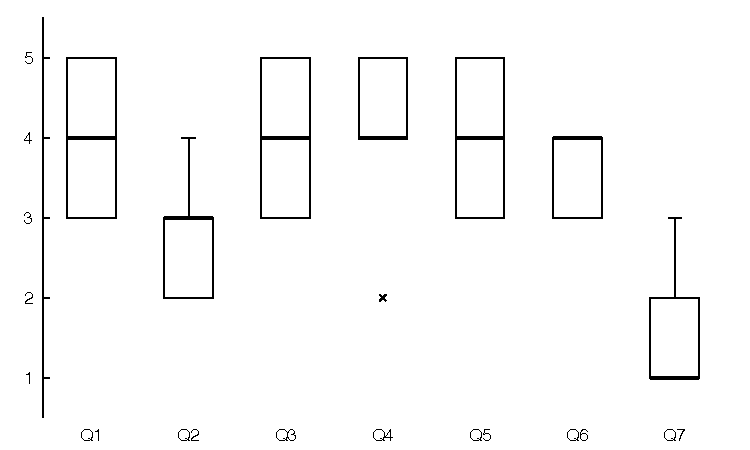
\includegraphics[width=0.7\textwidth]{../figures/boxplots/rwmpa-boxplot.pdf}
\caption[RWMPA Questionnaire Results]{RWMPA Questionnaire Results, 5-level Likert scale, Q1 workflow easy to understand, Q2 much manual work required, Q3 workflow reduced work effort, Q4 workflow guidance supported workflow understanding, Q5 task guidance supported task understanding, Q6 aware what is to do, Q7 manual configuration of tools}\label{fig:rwmpa.boxplot}
}
\end{figure}

\textbf{Analysis}.
In comparison to \gls{rewamp}, the time for manual interventions of the Prototyping Engineer was reduced from \(\overline{t_M}=\) 00:49:36h (\(\sigma =\) 00:10:06h \(\approx 20\% \overline{t_M}\)) in \gls{rewamp} to \(\overline{t_U}=\) 00:37:00h (\(\sigma =\) 00:05:43h \(\approx 15\% \overline{t_U}\)).
The time distribution across tasks in comparison to equivalent tasks of \gls{rewamp} \cref{tbl:rewamp-rwmpa} shows some differences.
In particular, the long time for \gls{rewamp} task 1 (BBL file extraction, mean 00:11:22h) was highly reduced in \gls{rwmpa} task 6 (select files, mean 00:01:11h) due to automatic dependency analysis in service task 5, reducing the complexity of user task 6 to mainly accepting or rejecting the automatic results.
Likewise, the time for the main activities of the Prototyping Engineer in \gls{rewamp}, task 4 (expert changes, mean 00:30:49h), and 5 (expert file, mean 00:05:06h), requiring an average of 00:35:55h in total, is reduced in \gls{rwmpa} workflow, in equivalent tasks 10 (delete code, mean 00:01:58h), 11 (replace code, mean 00:16:59) and 16 (expert changes, mean 00:08:30), with an average of 00:27:28h in total.
This can be an indication that the automatic suggestions for deletion and replacement autocompletion based on \gls{wasmt} provided methods based on the extended preprocessing in \gls{rwmpa} task 7 provided an acceleration for the expert interventions.
The apparent increase of the time for task 16 (expert changes) and of the correction cycles between \(u_{cal}\) and \(u_{new}\) is a consequence of differences between the two views in terms of dependencies already pointed out in \gls{rewamp} evaluation.
\vspace{-8pt}

The results of the subjective evaluation based on the test subjects' feedback shows a rather high agreement to the usefulness of the \gls{rwmpa} process guidance.
In particular, compared to \gls{rewamp}, the required sequence of tasks and the tasks themselves are better understood by the test subjects.
The higher degree of automation and the consistent \gls{ui} of \gls{rwmpa} for the underlying \gls{wasmt} toolchain can be seen in the low perceived manual configuration of migration tools.
\vspace{-8pt}

\textbf{Threats to Validity}.
Due to the high similarity of this experiment with the \gls{rewamp} experiment, the same threats to validity as in \cref{sec:rewamp.experiment} hold.
This paragraph outlines the differences concerning \emph{construct validity}.
Identical execution of the test runs was not only guaranteed due to the underlying formalized \gls{rwmpa} workflow but also through the \gls{rwmpa} process guidance.
Due to an error in time measurements, the test runs on \(u_{new}\) of two test subjects were not measured correctly.
To address this, measurements of these subjects on both test objects were excluded from the results.
As both test subjects, however, completed both test runs, their feedback in the questionnaire has been considered.
The comparisons between \gls{rewamp} and \gls{rwmpa} evaluation results should not be considered a comparative study since the test subjects were not the same.
While this was not feasible and subsequent test runs of \gls{rewamp} and \gls{rwmpa} would have influenced the measurements due to experience transfer, the test objects, i.e.~\(u_{cal}\) and \(u_{new}\) are identical.
\vspace{-8pt}

\textbf{Conclusion of RWMPA experimentation}.
The experiments have shown that \gls{rwmpa} can improve the \gls{rewamp} process of \gls{Rapid Web Migration Prototyping}.
In addition to the successful completion of all test runs as in the \gls{rewamp} experiment, observations showed a better understanding of the workflow and its tasks by the test subjects.
Due to the significantly extended guidance, they were aware of their context and what to do next and understood what was required in the tasks.
The increased degree of automation and support for performing the tasks has successfully reduced the required time, in particular for task 1.

\vspace{-10pt}
\hypertarget{sec:uitransformer.experiment}{%
\subsection{Experimental Evaluation of UI Transformer}\label{sec:uitransformer.experiment}}
\vspace{10pt}

The following experimental evaluation of UI Transformer focuses on two aspects: it explores the performance impact of the computational complexity of \gls{ui} \gls{Transformation} as well as perceived similarity and its influence factors in the transformed grid-based \glspl{wui}.

\textbf{Setup}.
The \emph{test dataset} \(L_T\) comprises 50 pixel-based \glslink{Legacy System}{legacy} layouts \(L_T = \{l_1, \ldots, l_{50}\}\) with different levels of complexity (amount of controls \(\#c\) between 2 and 130, \(\overline{\#c} = 22.42\)) and depth (levels of nesting \(d\) between 0 and 2, \(\overline d = 0.32\)) represented as \gls{mfc} resource files.
To reach the high variety required for testing the automatic \gls{Transformation}, these have been extracted from executables of various \glspl{Desktop Application} using Resource Hacker.
The test platform for the performance evaluation is an Intel Xeon E5-2670 CPU (2,6 GHz) with 16GB DDR3-1333 RAM running a minimal Arch Linux installation (Kernel version 4.15) without Desktop environment.
Hyperthreading supports 16 threads on 8 CPU cores.
For empirical evaluation, a subset \(L_T' \subset L_T\) of 5 layouts was used with complexity from 7 to 130 controls (\(\overline{\#c} = 8.24\), median \(\#\tilde c = 26\)).
The full test dataset \(L_T\) is used for performance analysis.
The questionnaire shown in \cref{sec:uitransformer-questionaire} was set up to capture subjective perceptions of the similarity of \glslink{Legacy System}{legacy} and transformed layouts in 7 criteria, each measured on a 5-level Likert scale of agreement.

\textbf{Procedure}.
For performance analysis, the full test dataset \(L_T\) was transformed with UI Transformer, and time measurements were taken.
Three times were measured corresponding to the three stages in \cref{fig:awsm.rm.uitransformer.horseshoe}: time for layout analysis \(t_A\), time for layout \gls{Transformation} \(t_T\) and time for layout generation \(t_G\).
Time \(t_T= t_0 + t_{opt} \) is further divided into the time for the initialization \(t_{0}\) and the time for the optimization \(t_{opt}\).
These times were measured programmatically using pythons \texttt{time} object with a precision of one millisecond.
Each test object (\glslink{Legacy System}{legacy} layout) was transformed using 11 different combinations of objective functions: 1 \(\{f_O, f_A\}\), 2 \(\{f_W, f_A, f_L\}\), 3 \(\{f_{D,H}, f_A, f_L\}\), 4 \(\{f_{D,G}, f_A, f_L\}\), 5 \(\{f_W, f_{D,H}, f_{D,G}\}\), 6 \(\{f_O\}\), 7 \(\{f_A, f_{W}, f_{D,G}\}\), 8 \(\{f_{D,H}, f_O\}\), 9 \(\{f_W, f_{D,G}, f_L\}\), 10 \(\{f_W, f_{D,H}, f_{D,G}, f_O, f_A, f_L\}\), 11 \(\{f_O\}\).
Combination 10 comprises all objective functions.
Combination 11 was measured on the C-based implementation to evaluate the potential for performance improvement.
The following parameters were used for the performance evaluation of each combination: 900 iterations of the evolutionary cycle, population size \(|P| = 30\), mating pool size \(|M| = 22\), recombination probability \(P_r = 0.5\), mutation probability \(P_m = 0.15\).

For empirical evaluation, \(L_T'\) was transformed to \(L_{T, grid}'\) using combinations 1-5.
Along with the initialisation approximation described in \cref{sec:uitransformation}, this created \(|L_{T, grid}'| = 5 \cdot(5+1)=30\) grid layouts for evaluation through test subjects.
Screenshots were taken from these layouts to ensure that all test subjects would see the same visual layout, independent of browser, platform, etc.
The study was conducted with 10 \emph{test subjects} with an age range of 21 to 52.
Each test subject was shown in random order pairwise combinations of a \glslink{Legacy System}{legacy} layout from \(L_T'\), and a corresponding transformed layout from \(L_{T, grid}'\) and was asked to rate the pair with regard to the seven questionnaire criteria for each pair.

\begin{longtable}[hbt]{@{}llllll@{}}
\caption[UITransformer Performance Evaluation]{\label{tbl:uitransformer.performance}UITransformer Performance Evaluation, all times but \(\sum\) in ms}\tabularnewline
\toprule
\textbf{Measure} & \textbf{Min} & \textbf{Max} & \textbf{Mean} & \(\bm{\sigma}\) & \(\bm{\sum}\) (mm:ss)\tabularnewline
\midrule
\endfirsthead
\toprule
Measure & Min & Max & Mean & \(\sigma\) & \(\sum\) (mm:ss)\tabularnewline
\midrule
\endhead
\(t_1\) & 13826 & 343834 & 60029 & 48040 & 14:31\tabularnewline
\(t_2\) & 11275 & 454761 & 75610 & 67207 & 19:39\tabularnewline
\(t_3\) & 19827 & 532608 & 107487 & 80564 & 26:12\tabularnewline
\(t_4\) & 26228 & 519752 & 111868 & 77746 & 26:17\tabularnewline
\(t_5\) & 32520 & 1040988 & 178444 & 152766 & 46:59\tabularnewline
\(t_6\) & 11046 & 312285 & 45344 & 42799 & 11:43\tabularnewline
\(t_7\) & 26766 & 745364 & 137568 & 111041 & 35:10\tabularnewline
\(t_8\) & 20692 & 635362 & 107390 & 91441 & 27:22\tabularnewline
\(t_9\) & 24792 & 663514 & 124481 & 98935 & 30:58\tabularnewline
\(t_{10}\) & 42196 & 1165719 & 206154 & 166035 & 50:47\tabularnewline
\(t_{11}\) & 62 & 15843 & 1501 & 2304 & 00:31\tabularnewline
\bottomrule
\end{longtable}
\textbf{Experimental results and descriptive statistics}.
The entire benchmark took about 2.5h to complete and produced 50 grid layouts as outputs, based on \(50\cdot 30\cdot 900 = 1.35\) million intermediate layouts in 900 generations.
\Cref{tbl:uitransformer.performance} shows the results of the performance evaluation per combination, aggregated over the 50 test objects; the detailed performance evaluation data is shown in \cref{tbl:uitransformer.fullperformance}.
\hypertarget{tbl:uitransformer.performance}{}

Each test subject contributed \(30 \cdot 7 = 210\) ratings, resulting in \(2100\) ratings overall, \(300\) per question in the questionnaire.
\Cref{fig:uitransformer.boxplot} shows the results of the questionnaire, the descriptive statistics on the averages aggregating the test subjects, layouts and combinations grouped by the 7 criteria are shown in \cref{tbl:uitransformer.empirical}; the detailed data is available in \cref{tbl:uitransformer.fullempirical}.
%\rule{0}{15\baselineskip}
%strut?
\begin{figure}[h!]
\hypertarget{fig:uitransformer.boxplot}{%
\centering
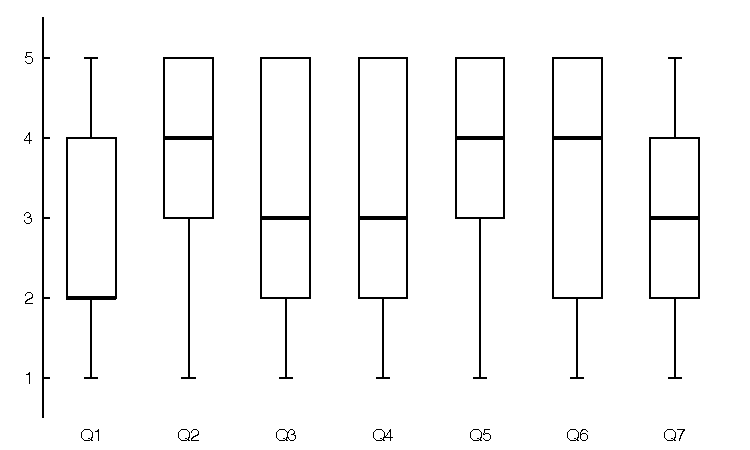
\includegraphics[width=0.7\textwidth]{../figures/boxplots/uitransformer-boxplot.pdf}
\caption[UI Transformer Questionnaire Results]{UI Transformer Questionnaire Results, 5-level Likert scale, Q1 same size, Q2 elements at least as large, Q3 left alignment consistent, Q4 right alignment consistent, Q5 same labels, Q6 same order, Q7 layouts identical}\label{fig:uitransformer.boxplot}
}
\end{figure}

\textbf{Analysis}.
The results show that layout \gls{Transformation} through evolutionary optimization is a computationally complex task due to the high number of iterations (900 generations) and intermediate results (1.35 million for 50 layouts) required.
The time is highly dependent on the combination of objective functions, varying from about 45s for the single-function combination 6 to 206s for combination 10 of all 6 objective functions, with some functions like \(f_W\) (compare \(t_2\) and \(t_3\)) having significantly less performance impact than others.
The measured times vary significantly not only between combinations but also within the measurements of the same combination.
For instance, \(t_6\) ranges from 11046ms to 312285ms, with a standard deviation of more than 0.94 of the mean.
These fluctuations are due to the different complexities of the user interfaces, which is the main influence factor on the \gls{Transformation} times.
The time measurements \(t_i\) and the number of controls \(\# c\) all show highly significant (\(\alpha = 0.001\)), very high correlations (Pearson's \(\rho \geq 0.945\), \(p < 3.28 \cdot 10^{-5}\) for all \(t_i\)).
The overall \gls{Transformation} time of about 2.5h for 50 user interfaces seems high.
However, this layout \gls{Transformation} is a one-time-only process that is not required to be run repeatedly.
The comparison between \(t_6\) and \(t_11\) shows that the potential performance increase through implementation in a low-level hardware-oriented platform like C can significantly accelerate the \gls{Transformation}.
\hypertarget{tbl:uitransformer.empirical}{}
\begin{xltabular}{0.75\linewidth}[h!]{@{}lllll@{}}
\caption{\label{tbl:uitransformer.empirical}UITransformer Empirical Evaluation}\tabularnewline
\toprule
\textbf{Criterion} & \textbf{Min} & \textbf{Max} & \textbf{Mean} & \textbf{\(\bm{\sigma}\)}\tabularnewline
\midrule
\endfirsthead
\toprule
\textbf{Criterion} & \textbf{Min} & \textbf{Max} & \textbf{Mean} & \textbf{\(\sigma\)}\tabularnewline
\midrule
\endhead
Q1 & 1.5 & 3.9 & 2.59 & 0.65\tabularnewline
Q2 & 2.8 & 4.6 & 3.92 & 0.42\tabularnewline
Q3 & 1.2 & 5 & 3.11 & 1.14\tabularnewline
Q4 & 1.2 & 5 & 3.09 & 1.15\tabularnewline
Q5 & 2.1 & 5 & 3.77 & 0.79\tabularnewline
Q6 & 1.9 & 5 & 3.37 & 1.07\tabularnewline
Q7 & 1.5 & 4.9 & 2.85 & 0.97\tabularnewline
\bottomrule
\end{xltabular}
%\vspace{-30pt}
\stepcounter{page}

The empirical results show that the transformed grid layouts are rated only medium with regard to the 7 criteria.
In particular, criterion Q7 (agreement to ``the layouts are identical'') was rated with an average of 2.85 by the test subjects.
The perceived similarity was dependent on the layout complexity.
While for \(l_1\) (\(\#c=7\)) similarity was rated at 3.53, for \(l_5\) (\(\#c=130\)) it drops to 2.15.
There is a significant (at \(\alpha = 0.05\)) strong negative correlation between Q7 and \(\# c\) (\(\rho=-0.915, p=0.0294\)).
Combination 1 (\(\{f_O, f_A\}\)) was rated best by the test subjects (\(Q7_1=3.08\)), combination 5 \(\{f_W, f_{D,H}, f_{D,G}\}\) received the lowest rating (\(Q7_5=1.94\)).
The highest similarity rating overall was achieved by the initial approximation (\(Q7_6=4.1\)).
A comparison of Q7 with the other criteria allows identifying influences on the similarity perception of the test subjects.
Kendall tau ranking correlation analysis was used for this aspect.
The strongest correlations exist with Q6 (``elements have the same order'', Kendall's \(\tau = 0.605\), \(p<10^{-3}\)) and Q5 (``elements are assigned with the same labels'', \(\tau = 0.522\), \(p<10^{-3}\)).
However, these correlations differ widely across test subjects: for test subject 1, the strongest correlation with Q7 is Q1 (\(\tau = 0.592\), \(p<10^{-3}\)), for test subject 3 it is Q3 (\(\tau = 0.657\), \(p<10^{-3}\)).
All correlations are highly significant at \(\alpha = 0.001\).

\textbf{Threats to Validity}.
\emph{Construct validity} of this experiment is mainly influenced by the difficulty to measure subjective similarity perceptions.
The seven criteria of the questionnaire attempt to map similarity onto concrete sub-aspects.
Interpretation of these aspects, however, is subjective.
This situation, however, is characteristic of empirical surveys on subjective perceptions.
Formulation of Q7 (``identical'') might have been too strong, leading to lower overall ratings compared to ``very similar''.
However, the main focus of the experiment was on comparative statements, as in the analysis above.
Rankings do not represent absolute values well.

\emph{Internal validity} of this experiment refers to potential biases.
While subjective biases from the researcher to the test subject were not a threat as there was no interaction between them during the experiment, some other factors are relevant.
Test subjects' understanding of criteria might have changed over the time of the experiment.
This was addressed by the relatively high number of overall rankings and the order randomization so that these effects are reduced by averaging.
Identical viewing conditions were ensured by providing screenshots of the layouts to avoid bias by rendering differences in different platforms, screen sizes, etc.

\emph{External validity} of the experiment is threatened through limitations in the generalizability of results.
The main factor is the test subjects, that are from a similar age range.
However, since subjective perceptions of similarity do not require specific knowledge or experience, evaluating with more test subjects might not significantly improve generalisability, similar to the Poisson relationship between test subjects and usability problems identified \autocite{Nielsen1993}, which also only requires relatively low numbers of test subjects without specific qualifications.
The second factor is the \glslink{Legacy System}{legacy} layout dataset \(L_T\), which provided the test objects for both performance and empirical evaluation.
To improve generalisability, these were taken from 6 different \glslink{Legacy System}{legacy} \gls{mfc} \glspl{Desktop Application} and representing a wide range of different layout complexities.

\textbf{Conclusion of UI Transformer Experimentation}.
The experimentation with UI Transformer has shown that the approach can be used to rapidly create grid-layout-based \gls{web} versions of pixel-based \glslink{Legacy System}{legacy} user interfaces.
The ordinal ranking scales from the empirical evaluation facilitated comparisons between different optimization variants.
The index approximations of the initial population (cf. \cref{eq:index-approximations}) were rated the highest with regard to similarity (\(Q7_6=4.1\) of 5), which means that it provides a reasonable quality that can be achieved with high performance.
Optimization comes at the cost of lower performance, but is still acceptable for a process run once and the acceleration potential of low-level programming languages has been demonstrated.
The experiment has shown that user interface similarity is not yet well understood and requires more research to map subjective similarity perceptions onto objectively measurable functions.
This is addressed in more detail in \cref{sec:awsm-ci}.
It was observed that the complexity of user interfaces plays a vital role in similarity perception and computational complexity.

Improved objective functions with regard to higher similarity and better performance can be easily integrated into the model-driven \gls{ui} \gls{Transformation} framework of UI Transformer to enhance the \glspl{web migration prototype} created by AWSM:RM.
An alternative would be an investigation of crowdsourcing layouts for \web migration prototyping as explored by Nebeling \autocite{Nebeling2012}, in particular as a tool-supported adaption process similar to CrowdAdapt \autocite{Nebeling2013CrowdAdapt} based on the initial index approximations.

\vspace{-10pt}
\hypertarget{sec:rm.evaluation.objective}{%
\subsection{Research Results}\label{sec:rm.evaluation.objective}}
\vspace{10pt}

The research objective addressed by this chapter, \cref{ro:2}, to enable demonstration of desirability and feasibility of a potential \glslink{web}{Web}-based version of the \gls{Legacy System} with limited resources and lack of \gls{Web Engineering} expertise, is achieved.
The effectiveness, efficiency, and expertise requirements of the AWSM:RM Method for creating a demonstrative \gls{web migration prototype} have been demonstrated and detailed in three different experiments.
The created prototypes are representing the main characteristics of \glspl{Web Application} and can be created with limited effort and expertise through reuse-focused techniques, automation, and guidance.
AWSM:RM RQ1 was answered through the prototyping approach presented in \cref{sec:rwmp}.
AWSM:RM RQ2 was answered through the introduction of the novel \gls{Rapid Web Migration Prototyping} strategy presented in \cref{sec:rwmp.overview} and the business logic reuse technique presented in \cref{sec:rewamp}.
AWSM:RM RQ3 was answered through the guidance system presented in \cref{sec:rwmpa} and the automated \gls{ui} transformation specified in \cref{sec:uitransformation}.

\vspace{-15pt}
\hypertarget{sec:rm.summary}{%
\section{Summary}\label{sec:rm.summary}}
\vspace{10pt}

This chapter presented the \gls{awsm} Risk Management Method, which facilitates the demonstration of feasibility and desirability of \gls{Web Migration} and the plausibility of a \glslink{web}{Web}-based version of the \gls{Legacy System}, specifying a novel \gls{Rapid Web Migration Prototyping} strategy.
This strategy is supported through a WebAssembly-based toolchain and has been enhanced with a guidance and automation system.
The conceptual model of the AWSM:RM techniques and their implementation in the Toolsuite have been described.
Evaluation comprising three separate experiments has shown the feasibility of the approach, quality of its results and low effort.
It has furthermore provided insights on activity complexity differences and suitable support mechanisms as well as on the need for research on the relation between subjective similarity perceptions and computable features, which is addressed in the following chapter.
